\documentclass[12pt]{article}
\usepackage[utf8]{inputenc}
\usepackage{amsmath, amsthm, mathtools, amsfonts, graphicx, hyperref,setspace, xparse, algorithm, algorithmicx, algpseudocode, mathabx, physics, tikz}

\usepackage{algorithm}
\usepackage{algpseudocode}

\usepackage[margin=1in]{geometry}

\usepackage{biblatex, tikz}
\addbibresource{bibliography.bib}

\theoremstyle{plain}% default
\newtheorem{theorem}{Theorem}[section]
\newtheorem{lemma}[theorem]{Lemma}
\newtheorem{prop}[theorem]{Proposition}
\newtheorem{ppties}[theorem]{Properties}
\newtheorem{cor}{Corollary}
\theoremstyle{definition}
\newtheorem{definition}{Definition}[section]
\newtheorem{example}{Example}[section]
\newtheorem{numexmp}{Numerical Example}[section]
\newtheorem{remark}{Remark}[section]
%\theoremstyle{remark}
%\newtheorem*{remark}{Remark}
\newtheorem*{note}{Note}
\newtheorem{case}{Case}

%\title{Hamiltonian Monte Carlo and Common Random Number}
\title{Common random number simulation as the optimal coupling for MCMC}
\author{Sabrina Sixta and Jeffrey S. Rosenthal}
\def\mc{Markov chain }
\def\sumn{\sum_{i=1}^n}
\def\andd{\bigcap}
\def\orr{\bigcup}
\def\io{\;\; i.o.}
\def\lfa{\leftrightarrow}
\def\ls{\lambda_*}
\def\wrt{with respect to }
\def\limn{\lim_{n\to \infty}}
\def\fld{\mathcal{F}}
\def\inn{\subseteq}
\def\supa{\sup_{A \subseteq S}}
\def\qd{q(\cdot,\cdot)}
\def\sump{\sum_{i=1}^p}
\def\vecx{\vec{X}}
\def\L{\mathcal{L}}
\def\X{\mathcal{X}}
\def\bbX{\boldsymbol{\X}}
\def\mcxn{\{X_n\}_{n\geq 1}}
\def\N{\mathbb{N}}
\newcommand{\indep}{\perp \!\!\! \perp}
\def\tin{\tau^{-1}}
\def\G{\Gamma}
\def\ax{p/2}
\def\bx{C/2}
\def\ay{(k+p)/2}
\def\by{C/2}
\def\tinv{\tau^{-1}}
\def\aax{1/2}
\def\bbx{S/2}
\def\aay{(J+2)/2}
\def\bby{S/2}
\def\borel{\mathcal{B}}
\def\unif{\mathrm{Unif}}
\def\bernoulli{\mathrm{Bernoulli}}
\def\d{\mathrm{d}}

\doublespacing

\begin{document}
	\maketitle
 \begin{abstract}
 	In this paper, we demonstrate that common random number simulation (CRN) applied to coordinate-wise monotone iterated random functions (IRF) represents the optimal Wasserstein coupling of an $n$-step Markov chain (MC). This finding generalizes the results of \cite{crn}, which establishes sufficient conditions for when CRN serves as the variance reduction coupling between functions of random variables. We provide specific examples of MCs where CRN is optimal, as well as cases where it is not. For those MCs where CRN does not yield the optimal coupling, we illustrate how CRN, applied to equimeasurable transformations, can still result in lower expected distances. Additionally, we argue why Wasserstein distance is the natural metric of choice when studying CRN and discuss the relationship between CRN, backward processes, and geometric convergence.
 \end{abstract}	
	\tableofcontents
	\addtocontents{toc}{\protect\setcounter{tocdepth}{2}}
\section{Introduction}
	%	\textbf{The fundamental problem with extending this to $\mathbb{R}^d, d>1$ is that there is no practical ordering in $\mathbb{R}^d$. Both of the following claim that optimality cannot be extended to $\mathbb{R}^d$ in a practical way: \href{https://arxiv.org/pdf/1803.00567}{Remark 2.30} and \href{https://link.springer.com/book/10.1007/978-3-319-20828-2}{Chapter 2 of this}}

Markov chain Monte Carlo (MCMC) is an integral part of statistical computing and Bayesian statistics is its most notable beneficiary \cite{honestexp,handbook}. An important question when simulating MCMC is how quickly does the chain converge to the stationary distribution of interest \cite{honestexp}. The Wasserstein distance, a measurement of distributions, is a popular method for evaluating whether a chain is close to stationarity \cite{wasmeth, gibbswass}. It scales well in high dimensions \cite{wasmeth} and metrizes convergence in distribution (see Theorem 6.9 of \cite{villani}).

Various methods for generating theoretical upper bounds on the Wasserstein distance between the distribution of a Markov chain and its stationary distribution exist \cite{wasmeth, wassdnm}. However theoretical bounds involve complex calculation, are difficult to implement, and do not exist for many MCMC models of interest \cite{waslinearmixedmodels,wassdnm,sixta,localcont}. 

An alternative method for estimating upper bounds on the Wasserstein distance is through common random number (CRN) simulation \cite{crn, jacob, sixtacrn} alternatively called synchronous coupling \cite{sdesynch,browniansynch, jacob}. CRN simulation translates to using the same random transform to generate two copies of a Markov chain (see Section \ref{sec:background} for more details) and is straightforward to implement. 

CRN simulation was proposed as the variance reduction coupling in as early as 1934 \cite{inequalities} and has been applied over a wide range of models including MCMC \cite{sixtacrn, biswas, crnconv}. In certain examples the contraction condition, which uses CRN (see Section \ref{subsec:backwardsprocess} for more details between the connection of CRN and the contraction condition), generates either the smallest geometric convergence rate \cite{oneshotnsphereexample, sixta,raj} or appears to be more tighter than drift and minorization bounds \cite{sixtacrn, jiangoneshotnsphereexample}.  

%If a Markov chain is average contractive, then the two copies of the chain simulated using CRN converge almost surely (Theorem \ref{thm:avcontcrn}). In this paper we show that if two copies of a Markov chain are increasing over the same regions, then the two copies of the chain simulated using CRN converge almost surely (Theorem \ref{thm:crnmc}) 

%CRN in MCMC applications appears to produce tight bounds even when a contraction rate is not established, but we still don't know why it works so well or the conditions for when CRN is an optimal coupling. The optimal coupling is the joint distribution that minimizes the expected distance between the distributions of two chains. 

CRN has been shown to be the optimal coupling for a variety of stochastic process examples. Namely, in \cite{browniansynch}, it is shown that under certain conditions two reflected Brownian motion processes simulated using CRN converge to 0 almost surely. In \cite{sdesynch} it is shown that CRN simulation is an optimal Wasserstein coupling between the solutions of SDEs. In \cite{independentmetropolishastings} it is shown that CRN simulation is the maximal total variation coupling on the independent Metropolis algorithm.

The optimality for CRN applied to MCMC was first discussed in \cite{crn}.
In $\mathbb{R}^d, d\geq 1$, Proposition 2.2 of \cite{crn} states that CRN applied to two coordinate-wise increasing transforms of two random variables minimizes the Euclidean distance. In this paper, we provide sufficient conditions for when CRN is an optimal Wasserstein coupling on the $n$th iteration of a Markov chain in $\mathbb{R}^d$ defined over general distances (see Theorem \ref{thm:crnmc}).  We generalize the results of \cite{crn} to quasi-antitone distance functions, show how CRN optimality can be applied to Markov chains, and add more details to the proof. 

%Brenier's theorem states that the optimal coupling on the Euclidean distance can be constructed through a non-decreasing function from the first random variable to the second. In Remark \ref{rem:brenier}, we sketch the relationship between the results of Brenier's theorem and Proposition 2.2 of \cite{crn}. Discussions related to CRN as the optimal coupling on random variables in $\mathbb{R}$ are also found in \cite{santambrogio, jacob}.


%In this paper, we provide sufficient conditions for when CRN is an optimal coupling on the $n$th iteration of a Markov chain in $\mathbb{R}^q, q\geq 1$ defined over general distances (see Theorem \ref{thm:crnmc}).  We generalize the results of \cite{crn} to quasi-antitone distance functions and provide more details to how optimality can be applied to Markov chains. 

We provide examples where CRN is the optimal coupling for a 1-step chain and an $n$-step chain. We show that CRN could be the optimal coupling for a 1-step chain, but not an $n$-step chain (see Example \ref{ex:randomlogmap} compared to Numerical Example \ref{numex:ranlogmap}). We also show that even though CRN is the optimal coupling for a 1-step chain, it does not necessarily imply that two copies simulated using CRN will converge in expectation (see Example \ref{ex:randomlogmap}). 

%In this paper we generalize and extend the results of \cite{crn} within the context of Wasserstein distance. We provide sufficient conditions for when CRN is an optimal coupling on the $n$th iteration of a Markov chain in $\mathbb{R}^q, q\geq 1$ defined over general distances (see Theorem \ref{thm:crnmc}). 

In section \ref{sec:invdf}, we start off by summarizing the useful properties of CRN when the random transform is the quantile function (aka the inverse distribution function). We justify why the Wasserstein distance is the natural measure for studying the convergence properties of random values simulated using CRN. In particular, for a Markov chain $\{X_n\}_{n\geq 1}$ defined in the metric space $(\mathcal{X},k)$, if we can write $X_n=F^{-1}_n(U_n)$ where $F_n$ is the distribution function of $X_n$ and $U_n\sim Unif(0,1)$, then applying CRN to two copies of a Markov chain means that convergence in distribution in $P_p(\mathcal{X})$ is equivalent to convergence in the $k$ mean when simulated using CRN (Proposition  \ref{thm:equivinv}). Further, convergence in distribution is equivalent to almost sure convergece of two chains simulated using CRN (Proposition \ref{thm:equivinv4}). 

In practice, we do not know the quantile function of $X_n$. Rather we define the Markov chain as a sequence of iterated random functions (IRF). That is, we can write $X_n=f(\theta_n,X_{n-1})$ where $\theta_n$ is a random variable. 
In Section \ref{sec:1step}, we identify when CRN is an optimal coupling on the first iteration of a Markov chain. In Theorem \ref{thm:rdrp} we show that if $f(\vec{\theta}_n,\vec{X}_{n-1})$ is increasing coordinate-wise for each $\theta_{i,n}\in \vec{\theta}_{n}$ for any $\vec{X}_{n-1}$ then CRN on the first iteration of a Markov chain is an optimal coupling.

In Section \ref{sec:nstep} we extend the results of Section \ref{sec:1step} to provide sufficient conditions for when CRN is the optimal coupling on the $n$th iteration of a Markov chain. In Theorem \ref{thm:crnmc} we show that if $f(\vec{\theta},\vec{x})$ is increasing coordinate-wise with respect to $ \vec{\theta}$ and $\vec{x}$, then CRN on the $n$th iteration of a Markov chain is an optimal coupling. This means that if two copies of a Markov chain, $\{\vec{X}_n\}_{n\geq1}$ and $\{\vec{Y}_n\}_{n\geq1}$, converge in distribution to a stationary distribution $\pi$, then $k(\vec{X}_n,\vec{Y}_n)$ converges in probability to 0 when generated by CRN (see Corollary \ref{cor:convprob}). If two copies of a Markov chain, $\{\vec{X}_n\}_{n\geq1}$ and $\{\vec{Y}_n\}_{n\geq1}$, are geometrically ergodic, then $k(X_n,Y_n)$ converges almost surely to 0 when generated by CRN (see Corollary \ref{cor:convwp1}).

In Section \ref{subsec:backwardsprocess}, we establish the connection between CRN and backwards processes by showing in Theorem \ref{thm:backwards} that the expected distance between the two coupled chains is equal to the expected distance between the backwards process at iterations $n$ and $n+1$. We also cover how contraction rates implicitly assume CRN in the joint coupling. 

First we introduce notation in the Section \ref{sec:background}. This section should be referenced if the reader wants clarity on notation throughout the paper.
		
\section{Background}\label{sec:background}
\paragraph{Markov chain notation:}Let $\{X_n\}_{n\geq 1}$ be a Markov chain such that $X_n$ can be written as an iterative random function ie. $X_n=f(\vec{\theta}_n,X_{n-1})\in \mathbb{R}$ where $\vec{\theta}_n\in\mathbb{R}^d, n\geq 1$ are in the probability space $(\mathbb{R}^d, \mathcal{B}(\mathbb{R}^d), \mu)$. Note that $\vec{\theta}_n$ are i.i.d. w.r.t $n$ and independent w.r.t. $d$. That is, for i.i.d. random variables $(\vec{\theta}_1,\ldots, \vec{\theta}_n)=\Theta_n$ on the support $\mu$ and initial value $x_0$
\begin{equation}\label{eq:forward}
 X_n=f(\vec{\theta}_n,f(\vec{\theta}_{n-1},\ldots, f(\vec{\theta}_1,x_0)\ldots ))=f_n(\Theta_n,x_0)
\end{equation} 
Any time-homogeneous Markov chain can be represented as an IRF \cite{avcont}. $X_n$ is the value of the Markov chain at iteration $n$.

%The function $f$ is considered to be monotone (preserve order) in $x$, if $x_1\leq x_2$ $\pi$-a.e. implies  
%\begin{equation}
%	f(\vec{\theta},x_1)\leq f(\vec{\theta},x_2) \text{ $\mu$-a.e.}
%\end{equation}
%The function $f$ is considered to be monotone in $\theta_i$, if for all $\theta_{i,1}\leq \theta_{i,2}$ $\mu_i$-a.e. 
%\begin{equation}
%	f((\theta_1,\ldots,\theta_{i,1},\ldots, \theta_d),x)\leq f((\theta_1,\ldots,\theta_{i,2},\ldots, \theta_d),x) \text{ $\mu_{-i}$-a.e. and $\pi$-a.e.}
%\end{equation} 
%
%The function $f$ is considered to be monotone in $\theta$, if it is monotone for all $\theta_i$.

% \cite{strassensthm, monotonicity}. Preserving order is also sometimes called realizing the monotonicity over the set of probability measures on $X_n$ and subsequently means that the set of probability measures on $X_n$ are realizably monotone \cite{fill2002}.

%We assume that $\{X_n\}_{n\geq 1}$ is $\phi$-irreducible, aperiodic and has stationary distribution $\pi$. 
%So that $\mathcal{L}(X_n)\to\pi$ where 
$\mathcal{L}(X_n)$ denotes the law of $X_n$ and $\mathcal{L}(X_n)\to\pi$ denotes weak convergence of the law of $X_n$ to a stationary distribution $\pi$.

%We assume that $f(\cdot,z)$ is a measurable, right continuous function with respect to $\theta$. We denote $I_z, D_z$ as two subsets of $\mathbb{R}$ where
%\begin{itemize}
%	\item $I_z$ represents the regions of $\theta$ where $f(\theta,z)$ is non-decreasing. That is, $$I_z=\{\theta\in \mathbb{R} \mid  \exists \epsilon>0 \text{ s.t. }\forall \theta_1,\theta_2\in B_{\epsilon}(\theta) \text{, if }\theta_1<\theta_2 \text{ then }f(\theta_1,z)\leq f(\theta_2,z)\}$$
%	\item $D_z$ represents the regions of $\theta$ where $f(\theta,z)$ is non-increasing. That is, $$D_z=\{\theta\in \mathbb{R} \mid  \exists \epsilon>0 \text{ s.t. }\forall \theta_1,\theta_2\in B_{\epsilon}(\theta) \text{, if }\theta_1<\theta_2 \text{ then }f(\theta_1,z)> f(\theta_2,z)\}$$
%\end{itemize} 
%
%Note that $I_z\cup D_z\subseteq \mathbb{R}$ and $I_z\cap D_z=\{\theta\in \mathbb{R} \mid  \exists \epsilon>0 \text{ s.t. }\forall \theta_1,\theta_2\in B_{\epsilon}(\theta) \text{, if }\theta_1<\theta_2 \text{ then }f(\theta_1,x)= f(\theta_2,x)\}$.

%\begin{lemma}\label{lem:countable}
%	If $f$ is CADLAG (right continuous and has a left limit), then $I_z$ and $D_z$ can be written as a countable union of disjoint intervals. That $I_z=\dot{\bigcup}_{n\geq 1}B_n$ and $D_z=\dot{\bigcup}_{n\geq 1}B'_n$ where $B_{n},B'_n\subset \mathbb{R}$ are intervals.
%	
%\begin{proof}
%	Denote the set $A_n\subset C_{f}\bigcap [n,n+1)$ ($C_{f}$ is the set of continuous points over the function $f$) as follows
%	$$A_n=\{a\in C_{f}\bigcap [-n,n) \mid \text{$\exists \epsilon >0$ $s.t. \forall \theta\in (a-\epsilon,a), f(\theta)>f(a)$ and  $\forall \theta\in (a,a+\epsilon), f(\theta)\geq f(a)$}\}$$
%	
%	We want to show that $A_\infty=\bigcup_{n\in\mathbb{Z}} A_n$ is countable.
%	
%	Next denote $\epsilon_a =\sup\{\epsilon>0\mid \text{ if } a-\epsilon<\theta<a, f(\theta)>f(a) \text{ and for } a<\theta<a+\epsilon, f(\theta)\geq f(a) \text{ and } B_{\epsilon}(a)\in C_{f(\cdot)}\}$. 
%	
%	Let $b,a\in A_n$ such that $b\neq a$. If $b\in B_{\epsilon_a}(a)$, then $a\notin B_{\epsilon_b}(b)$:
%	\begin{itemize}
%		\item If $b<a$ then $a-\epsilon<b<a$, $f(b)>f(a)$, at the same time for any $c$ such that $b<c<b+\epsilon_b$, $f(c)\geq f(b)$ and so $a\notin B_{\epsilon_b}(b)$
%		\item If $b>a$, then $a<b<a+\epsilon_a$, $f(b)\geq f(a)$. At the same time, for any $c$ such that $b-\epsilon_b<c<b$, $f(c)>f(b)$ and so $a\notin B_{\epsilon_b}(b)$
%	\end{itemize}
%	Thus $|a-b|\geq min\{\epsilon_a,\epsilon_b\}$. This means that $|\{a\in A_n \mid \epsilon_a\geq \frac{1}{m}\}|\leq m+1$ is finite. Next, note that $A_n\subset \bigcup_{m\geq 1} \{a\in A_n \mid \epsilon_a\geq \frac{1}{m}\}$, so it is countable. Finally,  $A_{\infty}=\dot{\bigcup}_{n\in \mathbb{Z}}A_n$ is a countable union of a countable union of finite sets, meaning that $A_{\infty}$ is countable.
%	
%	Suppose we order $a_n,a_{n+1}\in A_\infty\bigcup D_{f}$ (cannot prove this) such that $a_n<a_{n+1}$ and there are no values of $A_\infty\bigcup D_{f}$ in $(a_n,a_{n+1})$, (ie. $(A_\infty\bigcup D_{f})\bigcap [a_n,a_{n+1})=\emptyset$). Within the interval $[a_n,a_{n+1})$ there is exactly 1 interval, $B_n\in I_z$. If there were more than one, then there would exist a point $a'$ and an $\epsilon'>0$ such that for all $\theta\in (a'-\epsilon',a'), f(\theta)>f(a')$ and for all $\theta\in (a',a'+\epsilon'), f(\theta)\geq f(a')$. That is, $a'\in A_{\infty}$. A contradiction. Thus, there is a mapping between a sequence of disjoint intervals $\{B_n\}_{n\geq 1}$ and $A_\infty\bigcup D_{f}$ that covers $[\inf A_\infty\bigcup D_{f}, \sup A_\infty\bigcup D_{f})$. If the set $[\inf A_\infty\bigcup D_{f}, \sup A_\infty\bigcup D_{f})$ is bounded then we add two more intervals, $B'_1,B'_2$, that would be subsets of $(-\infty, \inf A_\infty\bigcup D_{f}]$ and $[\sup A_\infty\bigcup D_{f},\infty)$. Thus, we can construct a sequence of disjoint intervals $B'_1\bigcup B'_2 \bigcup_{n\geq 1}B_n=I_z$.
%	
%	By similar reasoning $D_z$ can be constructed as a countable union of disjoint intervals.
%\end{proof}
%\end{lemma}
%
%\begin{lemma}\label{lem:complementcountable}
%	If $f$ is CADLAG (right continuous and has a left limit), then $I_z^C$ and $D_z^C$ can be written as a countable union of disjoint intervals. That $I_z^C=\dot{\bigcup}_{n\geq 1}B_n$ and $D_z=\dot{\bigcup}_{n\geq 1}B'_n$ where $B_{n},B'_n\subset \mathbb{R}$ are intervals.
%	
%	\begin{proof}
%		
%		Denote $$A_{\infty}=\{a \in C_f\mid \text{$\exists \epsilon >0$ $s.t. \forall \theta\in (a-\epsilon,a), f(\theta)\leq f(a)$ and  $\forall \theta\in (a,a+\epsilon), f(\theta)> f(a)$}\}$$
%		
%		$A_{\infty}$ is countable using similar reasoning to the proof of Lemma \ref{lem:countable}. 
%		
%		Suppose we order $a_n,a_{n+1}\in A_\infty\bigcup D_{f}$ such that $a_n<a_{n+1}$ and there are no values of $A_\infty\bigcup D_{f}$ in $(a_n,a_{n+1})$, (ie. $(A_\infty\bigcup D_{f})\bigcap [a_n,a_{n+1})=\emptyset$). Within the interval $[a_n,a_{n+1})$ there is exactly 1 interval, $B'_n\in I_z$. If there were more than one, then there would exist a point $a'$ and an $\epsilon'>0$ such that for all $\theta\in (a'-\epsilon',a'), f(\theta)\leq f(a')$ and for all $\theta\in (a',a'+\epsilon'), f(\theta)> f(a')$. That is, $a'\in A_{\infty}$. A contradiction. Thus, there is a mapping between a sequence of disjoint intervals $\{B'_n\}_{n\geq 1}$ and $A_\infty\bigcup D_{f}$ that covers $[\inf A_\infty\bigcup D_{f}, \sup A_\infty\bigcup D_{f})$. 
%		
%		By similar reasoning $I_z^C$ can be constructed as a countable union of disjoint intervals.
%	\end{proof}
%\end{lemma}
%\begin{lemma}
%	The set $A =(I_x\cap I_y)\cup (D_x\cap D_y)$ can be written as countably many intervals.
%	
%	\begin{proof}
%		By Lemma \ref{lem:countable}, the sets $I_x,I_y,D_x,D_y$ can be written in terms of countably many intervals:
%		\begin{align*}
%			& I_x=\dot{\bigcup}_{n\geq 1}B_{x,n} & I_y=\dot{\bigcup}_{n\geq 1}B_{y,n}\\
%			& D_x=\dot{\bigcup}_{n\geq 1}B'_{x,n} & D_y=\dot{\bigcup}_{n\geq 1}B'_{y,n}
%		\end{align*}
%		
%		Where $B_x,n$ are intervals.
%		
%		Thus, $A_n=(\dot{\bigcup}_{n\geq 1}\dot{\bigcup}_{m\geq 1}B_{x,n}\bigcap B_{y,m})\bigcup (\dot{\bigcup}_{n\geq 1}\dot{\bigcup}_{m\geq 1}B'_{x,n}\bigcap B'_{y,m})$, the terms $B_{x,n}\bigcap B_{y,m}$ and $B'_{x,n}\bigcap B'_{y,m}$ are intervals which means that $A_n$ can be written as a countable sequence of intervals.
%	\end{proof}
%\end{lemma}	

%\begin{lemma}
%	Let $A =(I_x\cap I_y)\cup (D_x\cap D_y)$. The sets $A \setminus (I_x\cap I_y)$ can be written as countably many disjoint intervals.
%	
%	\begin{proof}
%		
%	
%	\end{proof}
%\end{lemma}	

The Markov chain $\{\vec{X}_n\}_{n\geq 1}\in \mathbb{R}^q, q\geq 1$ is a vector form of the initial chain where for each vector coordinate $i\in\{1,\ldots, q\}$ we have $X^{(i)}_n=f^{(i)}(\vec{\theta}_n,\vec{X}_{n-1})$.  
 \paragraph{CRN} CRN simulation occurs when we simulate two Markov chains $\{X_n\}_{n\geq 1}$ and $\{Y_n\}_{n\geq 1}$ with different initial values $x_0\neq y_0$, but with the same transition functions. That is, $\vec{\theta}_n$ are the same in $X_n = f(\vec{\theta}_n,X_{n-1})$ and $Y_n = f(\vec{\theta}_n,Y_{n-1})$, $n\geq 1$. In different notation, $\Theta_n$ is the same in $X_n = f_n(\Theta_n,x_0)$ and $Y_n = f_n(\Theta_n,y_{0})$, $n\geq 1$. CRN is unique to the IRF, but not the the Markov chain \cite{crn}. Some texts limit CRN to the inverse transform of the distribution function \cite{crn,jacob} like what is done in Section \ref{sec:invdf}.
 
\paragraph{Distance function $k$:}Let $k$ be a distance function. 

$k$ is quasi-antitone (in other words $-k$ is supermodular) if for all $x\leq x'$, $y\leq y'$ $\pi$-a.e.,
$$k(x,y)+k(x',y')-k(x,y')-k(x',y)\leq 0$$
We will need $k$ to be quasi-antitone to prove that CRN is an optimal coupling. We write that $k$ is QAC if $k$ is a quasi-antitone continuous distance function. 

%$k$ is sign-invariant if for all $x,y$ $\pi-$ a.e. $k(x,y)=k(-x,-y)$.

Theorem 3 of \cite{rearrangefunc} tells us that functions $f(x-y)$ where $f$ is convex and $f(0)=0$ are QAC. The $\ell^p$ norm is defined as follows, $||\vec{x}||_p=\left(\sum_{i=1}^q x_i^p\right)^{1/p}$ and is a QAC distance function. 

% See chapter 6 c of file:///C:/Users/User/Downloads/978-0-387-68276-1.pdf for sub-modular in $\mathbb{R}^d$.

%Assume that $k$ is convex, that is for any $t\in(0,1)$ and $(x,y), (x',y')$ $\pi$-a.e.,
%$$k(t(x,y)+(1-t)(x',y'))\leq tk(x,y)=(1-t)k(x',y')$$
%We need $k$ to be convex so that....

%\paragraph{Wasserstein distance} Let $(\mathcal{X},\mathcal{F})$ be a measurable space with metric $d$.
%The $k$ Wasserstein distance between distributions $\mu,\nu$ on $(\mathcal{X},\mathcal{F})$ is defined as,
%%	$$W_p(\pi,\mu)=\inf_{(X,Y)\sim J(X,Y)}E[d_p(X,Y)^p]^{1/p}$$
%$W_{k}(\mu,\nu)=\inf_{X\sim \mu, Y\sim \nu}E[k(X,Y)]$. 

\paragraph{Wasserstein distance} We define $J(X,Y)$ as a joint distribution function of $X,Y$ and $\mathcal{J}(\mu,\nu)=\{J(X,Y)\mid \mathcal{L}(X)=\mu, \mathcal{L}(Y)=\nu \}$ to be the set of all joint distribution functions with marginals $\mu,\nu$. 
%The Wasserstein distance of order $p\in [1,\infty)$ between distributions $\mu,\nu$ on the metric space $(\mathcal{X},k)$ is defined as,
%$W_{p}(\mu,\nu)=\inf_{X\sim\mu,Y\sim\nu}E_J[k(X,Y)^p]^{1/p}$
 The Wasserstein distance of order $p$ is 
$W_{k,p}(\mu,\nu)=\inf_{J\in \mathcal{J}(\mu,\nu)}E_J[k(X,Y)^p]^{1/p}$ for $p\in [1,\infty)$.

$J\in \mathcal{J}(\mu,\nu)$ is an optimal coupling if $E_J[k(X,Y)^p]^{1/p}=W_{p}(\mu,\nu)$ \cite{villani}. That is $J$ is the joint distribution such that the expected distance between $X$ and $Y$ using joint distribution $J$ is equal to the Wasserstein distance.

We define the Wasserstein space of order $p$, $P_p(\mathcal{X})$, as the space of Borel probability measures on the metric space $(\mathcal{X},k)$ such that for any $\mu\in P_p(\mathcal{X})$, $\int_{\mathcal{X}}k(x_0,x)^p
\mu dx <\infty$ for some $x_0\in \mathcal{X}$.

Define a sequence of random variables $\{X_n\}_{n\geq 1}$ in a Polish metric space $(\mathcal{X},k)$ with distributions in $\mathcal{L}(X_n)\in P_p(\mathcal{X})$. Define $\mathcal{L}(X)=\pi\in P_p(\mathcal{X})$. $X_n$ converges weakly to $\pi$ in $P_p(\mathcal{X})$ (denoted as $\mathcal{L}(X_n)\to \pi$ in $P_p(\mathcal{X})$) if (1) $\mathcal{L}(X_n)\to \pi$ and (2) for some $x_0\in \mathbb{R}$, $E[k(x_0,X_n)^p]\to E[k(x_0,X)^p]$ (see alternative conditions in Definition 6.8 of \cite{villani}).

%\begin{prop}{Wasserstein distance metrizes convergence in distribution (Theorem 6.9 of \cite{villani})}\label{prop:wassandweak}
%	Define a sequence of random variables $\{X_n\}_{n\geq 1}$ in a Polish metric space $(\mathcal{X},k)$ with distributions in $\mathcal{L}(X_n)\in P_p(\mathcal{X})$. Define $X\sim \pi$ as the stationary random variable. Then  $\mathcal{L}(X_n)$ converges weakly to $\pi$ in $P_p(\mathcal{X})$ if and only if the Wasserstein distance converges to $0$ (Theorem 6.9 of \cite{villani}),
%	\begin{equation}
%		\mathcal{L}(X_n)\to \pi \text{ in } P_p(\mathcal{X})\iff W_{k}(\mathcal{L}(X_n), \mathcal{L}(X))\to 0
%	\end{equation}
%\end{prop}

%\subsection{Connection between CRN and the contraction condition}\label{subsec:contractioncond}
%%Within a Markov chain $\{X_n\}_{n\geq 1}$ in $(\mathcal{X},\mathcal{F})$ such that $X_n = f_{\theta_n}(X_{n-1})$, where  $\{\theta_n\}_{n\geq 1}$ are i.i.d. random variables on some measurable space $\Theta$ and random measurable mappings $f_{\theta_n} : \mathcal{X} \mapsto \mathbb{R}$. The set of random functions $f_{\theta_1}, f_{\theta_2},\ldots$ is called an iterated function system. Any time-homogeneous Markov chain can be represented as an iterated function system \cite{avcont}.
%In this subsection, we will show that CRN is the joint distribution that generates the contraction condition, which is a sufficient condition for geometric ergodicity. 
%
%%Suppose $\{X_n\}_{n\geq 1}$ is a Markov chain such that $X_n = f(\theta_n, X_{n-1})$ where $\theta_n$ are i.i.d. random variables. That is, $X_n$ can be written as follows,
%%\begin{equation}\label{eq:forward}
%%	X_n = f(\theta_n,(f(\theta_{n-1},\ldots f(\theta_1,X_0)))
%%\end{equation}
%%Further suppose that the corresponding stationary distribution is $\pi$ and that $\mathcal{L}(X_n)\to \pi$. 
%
%\paragraph{Geometric ergodicity } A Markov chain is called geometrically ergodic if there exists a $\gamma\in (0,1)$ and $M(x)<\infty$ for $\pi-$a.e. $x$ such that
%\begin{equation}\label{eq:geomerg}
%W_p(\mathcal{L}(X_n),\pi)\leq M(x_0)\gamma^n
%\end{equation}
%
%The rate of converge, $\gamma^*\in (0,1)$ is the infimum $\gamma$ such that for any $x_0$ equation \ref{eq:geomerg} holds. We are typically interested in determining when a Markov chain is geometrically ergodic and finding an upper bound on $\gamma^*$. 
%
%\begin{definition}[Average contractive]
%	A Markov chain is average contractive if for all $x,y$ $\pi-$everywhere,
%	$$\gamma_{cont}=\sup_{x \not= x'} \frac{E[k(f(\theta, x),f(\theta, x'))]}{k(x,x')}<1$$
%\end{definition}
%
%The value $\gamma_{cont}$ is called the contraction rate and is an upper bound on $\gamma^*$. Modifications to the contraction condition have been widely studied and can be found in \cite{iteratedranfunc, ifssurvey, tweedielocalcont, ifssurvey1, localcont, avcont}. The random logistic map (Example \ref{ex:randomlogmap}) and Zeno's walk (Example \ref{ex:zeno}) are locally contractive \cite{localcont}, which is weaker than average contractive.
%
%\begin{theorem}\label{thm:avcontcrn}
%	If $\gamma_{cont}<1$, then two copies of the Markov chain simulated using CRN converge almost surely. 
%	\begin{proof}
%		If $\gamma_{cont}<1$, then for all $x,y$ $\pi-$everywhere,
%		$E[k(f(\theta, x),f(\theta, x'))] \leq \gamma_{cont}k(x,x')$. This means that at iteration $n$, $E[k(f_n(\Theta_n, x_0),f_n(\Theta_n, x'_0))] \leq \gamma_{cont}^nk(x_0,x'_0)$.
%		
%		Let $\epsilon>0$
%		\begin{align*}
%			\sum_{n=0}^{\infty}P(k(f_n(\Theta_n,x_0),f_n(\Theta_n,x'_0))>\epsilon)&\leq 	\sum_{n=0}^{\infty}\frac{E[k(f_n(\Theta_n,x_0),f_n(\Theta_n,x'_0))]}{\epsilon}\\
%			&\leq \sum_{n=0}^{\infty}\frac{\gamma_{cont}^nk(x_0,x'_0)}{\epsilon}\\
%			&=\frac{k(x_0,x'_0)}{\epsilon(1-\gamma_{cont})}\\
%			&<\infty
%		\end{align*}
%		By the Borel-Cantelli Lemma, $P(k(f_n(\Theta_n,x_0),f_n(\Theta_n,x'_0))>\epsilon \text{ i.o.})=0$ for $\epsilon>0$, which is equivalent to saying that $P(\lim_{n\to\infty}k(f_n(\Theta_n,x_0),f_n(\Theta_n,x'_0))=0)=1$ by Lemma 5.2.1 of \cite{firstlook} and so $X_n, X'_n$ generated using CRN will converge almost surely. 
%	\end{proof}
%\end{theorem}
%
%%\begin{definition}[Global average contraction condition-CRN]\label{def:cont}
%%	An iterative function system is global average contractive if there exists a $\gamma\in (0,1)$ such that, $$\gamma \geq \sup_{x \not= x'} \frac{E[k(f(\theta, x),f(\theta, x'))]}{k(x,x')}$$
%%\end{definition}
%
%%Modifications to the above contraction condition have been widely studied and can be found in \cite{iteratedranfunc, ifssurvey, tweedielocalcont, ifssurvey1, localcont, avcont}. 
%
%Notice that the contraction rate implicitly uses CRN. That is, we apply the same $\theta$ in $f(\theta,x)$ and $f(\theta,x')$ to calculate the contraction rate. Contractions rates for examples  \ref{ex:arnormdep}, \ref{ex:locmodel}, \ref{ex:lineararch} have been calculated in \cite{sixta}. For the Bayesian location model (example \ref{ex:locmodel}) and the autoregressive normal process in $\mathbb{R}$ (example \ref{ex:arnormdep}), the contraction rate equals the rate of convergence, $\gamma_{cont}=\gamma^*$. See \cite{sixta} for more details.
%
%\subsection{Connection between CRN and backwards processes}\label{subsec:backwardsprocess}
%\paragraph{Backwards process }
%
%The backwards process coupled with contraction conditions are commonly used to establish theorems that generate upper bounds on the Wasserstein distance between the distribution of a Markov chain and its corresponding stationary distribution (see \cite{iteratedranfunc,avcont,localcont}).
%
%The backward process, $\{\tilde{X}_n\}_{n\geq 1}$, which is not a Markov chain \cite{localcont} but tends to converge pointwise to a limit, is defined as follows,
%\begin{equation}\label{eq:backward}
%	\tilde{X}_n = f(\theta_1,(f(\theta_{2},\ldots f(\theta_n,X_0)))
%\end{equation}
%The difference between the Markov chain and the backwards process is the order of $\theta_1,\theta_2,\ldots,\theta_n$ to generate the next iteration (see equation \ref{eq:forward} compared to equation \ref{eq:backward}). Figure \ref{fig:backwardsvsforwards} graphs the forward and backward process of an autoregressive process using the same random mappings. The point towards which the backwards process converges is itself random. 
%
%\begin{figure}
%	\centering
%	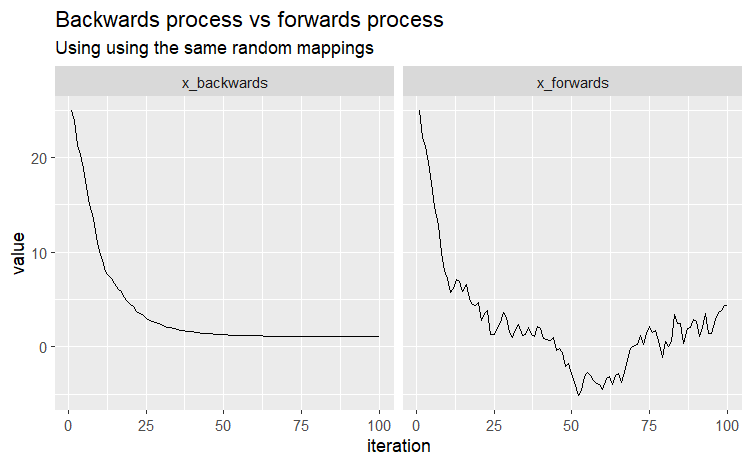
\includegraphics[width=0.7\linewidth]{images/backwardsvsforwards}
%	\caption{The backwards, $\{\tilde{X}_n\}_{n\geq 1}$, and forwards, $\{X_n\}_{n\geq 1}$, process of the autoregressive normal system where $X_n,\tilde{X}_n$ are simulated using the same random mappings, $X_n=0.9X_{n-1}+Z_n, Z_n\sim N(0.1)$ and $X_0=25$.}
%	\label{fig:backwardsvsforwards}
%\end{figure}
%
%%The forward process, $\{X_n\}_{n\geq 1}$, which is a Markov chain, is defined as follows,
%%$$X_n = f(\theta_n,(f(\theta_{n-1},\ldots f(\theta_1,X_0)))$$
%
%%The backward process, $\{\tilde{X}_n\}_{n\geq 1}$, which is not a Markov chain \cite{localcont} but tends to converge pointwise to a limit, is defined as follows,
%%$$\tilde{X}_n = f(\theta_1,(f(\theta_{2},\ldots f(\theta_n,X_0)))$$
%
%%The difference between the two processes is the order of $\theta_1,\theta_2,\ldots,\theta_n$ to generate the next iteration. Figure \ref{fig:backwardsvsforwards} graphs the forward and backward process of an autoregressive process using the same random mappings. The point towards which the backwards process converges is itself random. 
%
%
%Despite the difference in behaviour of the two processes, the marginal distributions of the forward and backward processes are the same, $X_n \overset{d}{=}\tilde{X}_n$. In fact, the expected distance over the joint distribution of $J(\bar{X}_n,\bar{X}_{n+1})$ realizes the same expected distance as the $J(X_n,X'_n)$ when CRN is used. 
%
%\begin{theorem}\label{thm:backwards}
%	Let $X_n,Y_n$ be two copies of a Markov chain such that $X_n=f(\theta_n, X_{n-1})$ and $Y_n=f(\theta'_n, Y_{n-1})$. Suppose that $X_0=x$ and $Y_0=f(\theta,x)$ where $\theta\indep \theta_i, \theta'_i$ for $i\in\{1\ldots, n\}$, then the expected distance between $X_n$ and $Y_n$ using CRN is equal to the expected distance between consecutive iterations of the backwards process, $\bar{X}_n$ and $\bar{X}_{n+1}$.
%	$$E[d(X_n,Y_{n})\mid X_0=x]=E[d(\tilde{X}_n,\tilde{X}_{n+1})\mid \tilde{X}_0 = x]$$ 
%	\begin{proof}
%		\begin{align*}
%			&E[d(X_n,Y_{n})\mid X_0=x] \\
%				&=E[d[f(\theta_n,f(\theta_{n-1},\ldots f(\theta_1,x)\ldots)),f(\theta_n,f(\theta_{n-1},\ldots f(\theta_1,f(\theta,x))\ldots))]\mid X_0=x]\\
%			&=E[d[f(\theta_n,f(\theta_{n-1},\ldots f(\theta_1,x)\ldots)),f(\theta_n,f(\theta_{n-1},\ldots f(\theta_1,f(\theta_{n+1},x))\ldots))]\mid X_0=x]\\
%			&=E[d[f(\theta_1,f(\theta_{2},\ldots f(\theta_n,x)\ldots)),f(\theta_1,f(\theta_{2},\ldots f(\theta_n,f(\theta_{n+1},x))\ldots))]\mid \tilde{X}_0=x]\\
%			&= E[d(\tilde{X}_n,\tilde{X}_{n+1})\mid \tilde{X}_0 = x]
%		\end{align*}
%	\end{proof}
%\end{theorem}
%
%This means that for initial values defined as in Theorem \ref{thm:backwards}, when CRN is an optimal coupling at iteration $n$, the expected distance between consecutive iterations of the backwards process is also an optimal coupling on the marginal distributions. Corollaries \ref{cor:convprob} and \ref{cor:convwp1} thus provide sufficient conditions for when the expected distance on the backwards process, $E[d(\tilde{X}_n,\tilde{X}_{n+1})]$, converges to $0$ in probability and almost surely, respectively.


\section{Applying CRN to quantile functions}\label{sec:invdf}
We first discuss the simplest case of CRN: when random variables $X,Y\in\mathbb{R}$ are written as the quantile transform of a uniform random variable. We define the quantile function as $F^{-1}(u)=\inf\{x\mid u\leq F(x)\}$, and our random variables as functions of the quantile function, $X=F^{-1}_x(U)\sim\mu$ and $Y=F^{-1}_y(V)\sim\nu$ where $U,V\sim Unif(0,1)$). We can specify the interval of expected values for distance $E[k(X,Y)]$ when $J\in \mathcal{J}(\mu,\nu)$  in Proposition  \ref{prop:interval}.

Proposition \ref{prop:interval} lays the foundation for the rest of the theorems in this paper. Namely Proposition \ref{prop:incr1} uses Proposition \ref{prop:interval} to prove that CRN is the optimal coupling when $X$ is an increasing function of $U$. 

Proposition \ref{prop:interval} is important for generalizing optimality properties of random variables simulated using CRN, because it specifies the set of distance functions $k$ where CRN is the optimal coupling.

\begin{prop}[Theorem 2 of \cite{cambanis1976}]\label{prop:interval}
		Suppose that $X,Y \in \mathbb{R}$ are two random variables with corresponding distribution functions $F_x, F_y$ such that $X\sim \mu$ and $Y\sim \nu$. Suppose that $k$ is QAC and that $\mu,\nu\in P_p(\mathbb{R})$. %Further assume that the expected distances are finite, $-\infty<E[k(F^{-1}_x(U),F^{-1}_y(U))]$ and $E[k(F^{-1}_x(U),F^{-1}_y(1-U))]<\infty$. 
		Then, the set of expected distances of $k(X,Y)$ with joint distribution $J\in \mathcal{J}(\mu,\nu)$ is equal to the following interval,
		$$\big\{E_J[k(X,Y)] \mid J\in \mathcal{J}(\mu,\nu) \big\}= \big[E[k(F^{-1}_x(U),F^{-1}_y(U))], E[k(F^{-1}_x(U),F^{-1}_y(1-U))] \big]$$
		\begin{proof}
		Note that condition $(a)$ of Theorem 2 of \cite{cambanis1976} is satisfied, because $k$ is symmetric and $\mu,\nu\in P_p(\mathbb{R})$ and so for some $x_0\in\mathbb{R}$, $E[k(X,Y)]\leq E[k(X,x_0)]+E[k(x_0,Y)]<\infty$. 	
		\end{proof}	
\end{prop}	

%Using a CDF function transform to maximize the covariance between two random variables in $\mathbb{R}$ was first described in \cite{inequalities}. Using a CDF function transform to minimize a quasi-antitone distance function between two random variables in $\mathbb{R}^d$ was defined in \cite{rearrangefunc}. 

%Next we show how, convergence in distribution also implies almost sure convergence when CRN is applied. This theorem can be seen as a corollary of Skorohod's theorem, since the proofs are nearly identical. 

%\begin{theorem}\label{thm:skorohod}
%	Let $\{X_n\}_{n\geq 1}$ and $\{Y_n\}_{n\geq 1}$ be two sequences of random variables in $\mathbb{R}$. Define the distributions of $X_n$ ($Y_n$) to be $F_{x,n}$ ($F_{y,n}$). If CRN is applied and both distribution functions converge to distribution function $F$, then 
%	$$|F_{x,n}^{-1}(U)-F^{-1}_{y,n}(U)|\to 0 \text{ w.p. 1}$$
%	
%	The proof is in Subsection \ref{pf:skorohod} and closely follows the proof of Skorohod's theorem (see Theorem 25.6 in \cite{billingsley}).
%\end{theorem}

Proposition \ref{thm:equivinv} summarizes why we focus on Wasserstein distance to study convergence of CRN applied to quantile functions. Namely, the Wasserstein distance metrizes weak convergence in $P_p(\mathbb{R})$. This along with the fact that in one dimension the Wasserstein distance admits the quantile representation, $W_p(\mu,\nu)
= E[k(F_\mu^{-1}(U), F_\nu^{-1}(U))^p]^{1/p}$ when $k$ is QAC means that CRN applied to the quantile function metrizes convergence in distribution in $P_p(\mathbb{R})$. 

%Proposition \ref{thm:equivinv} explains why we focus on Wasserstein distance when studying convergence of CRN applied to inverse distribution functions. 
%On $P_p(\mathbb{R})$, the Wasserstein distance $W_p$ metrizes weak convergence together with convergence of $p$th moments. 
%In one dimension, $W_p$ admits the quantile representation
%\[
%W_p^p(\mu,\nu)
%=
%\int_0^1 |F_\mu^{-1}(u) - F_\nu^{-1}(u)|^p \, du,
%\]
%and the inverse-CDF (CRN) coupling attains this infimum. 
%Consequently, convergence of the CRN-coupled inverse distribution functions in $L^p(0,1)$ is equivalent to convergence in Wasserstein distance.

%Why is this important? Because it signals that the Wasserstein distance is the natural measure to study convergence of random variables simulated using CRN. This is in contrast with total variation distance, which does not metrize convergence in distribution and requires the probability that two random variable are equal to converge to 1. However, CRN applied to random variables in $\mathbb{R}$ usually does not lead to equality resulting in a non-convergent total variation distance.

The importance of this observation lies in the fact that it identifies the Wasserstein distance as a natural metric for studying convergence of random variables generated via CRN. This is in contrast to the total variation distance, which is the metric used to analyze CRN convergence in \cite{crnconv,independentmetropolishastings}. Total variation distance does not metrize convergence in distribution. Indeed, convergence in total variation distance requires that $P(X=Y)\to 1$, which is equivalent to the existence of a coupling under which the two random variables become equal with probability tending to one. In most applications of CRN for real-valued random variables, however, the coupled variables are not equal almost surely; rather, they are constructed to be strongly positively dependent.
\begin{prop}\label{thm:equivinv}
	Define the random variables $\{X_n\}_{n\geq 1}$ and $X$ in a Polish metric space $(\mathbb{R},k)$.% such that $\sup_{n}E[k(X_n,x_0)^p]<\infty$.
	The following are equivalent where $U\sim \unif(0,1)$.
	\begin{enumerate}
		\item $\mathcal{L}(X_n)\to \pi \text{ in } P_p(\mathbb{R})$
		\item $W_{p}(\mathcal{L}(X_n), \mathcal{L}(X))\to 0$
		\item $E[k(F^{-1}_{X_n}(U),F^{-1}_{X}(U))^p]^{1/p}\to 0$
	%	\item $|F^{-1}_{X_n}(U)-F^{-1}_{X}(U)| \to 0$ w.p. 1
	\end{enumerate}
	
	\begin{proof}
		%First note that since $\sup_{n}E[k(X_n,x_0)]<\infty$, $X_n\in P_p(\mathbb{R})$.% and $E[k(X,x_0)]<\infty$, $\mathcal{L}(X_n)$
		
		$(1)\iff (2)$: by Theorem 6.9 of \cite{villani}.
		
		$(2)\iff (3)$: By Proposition \ref{prop:interval}, the Wasserstein distance is attained when CRN is applied for each $n$,
		\begin{align*}
			W_p(\mathcal{L}(X_n), \mathcal{L}(X))&=\left(\inf_{J\in \mathcal{J}(\mathcal{L}(X_n), \mathcal{L}(X))} E_J[k(X_n,X)^p] \right)^{1/p}\\
			&=E[k(F^{-1}_{X_n}(U),F^{-1}_{X}(U))^p]^{1/p}
		\end{align*} %$W_p(\mathcal{L}(X_n), \mathcal{L}(X))=\left(\inf_{J\in \mathcal{J}(\mathcal{L}(X_n), \mathcal{L}(X))} E_J[k(X_n,X)^p] \right)^{1/p}=E[k(F^{-1}_{X_n}(U),F^{-1}_{X}(U))^p]^{1/p}$.
		 %Define $Y=\sup_n d(F^{-1}_{X_n}(U),x_0)+d(x_0,F^{-1}_{X}(U))$. Then $d(F^{-1}_{X_n}(U),F^{-1}_{X}(U))\leq Y$ and $E[Y]<\infty$. By the Dominated Convergence Theorem, $E[d(F^{-1}_{X_n}(U),F^{-1}_{X}(U))]\to 0$.
	\end{proof}
%	 Then  $\mathcal{L}(X_n)$ converges weakly to $\pi$ in $P_p(\mathcal{X})$ if and only if the Wasserstein distance converges to $0$ (Theorem 6.9 of \cite{villani}),
%	\begin{equation}
%		\mathcal{L}(X_n)\to \pi \text{ in } P_p(\mathcal{X})\iff W_{k}(\mathcal{L}(X_n), \mathcal{L}(X))\to 0
%	\end{equation}
\end{prop}

Proposition \ref{thm:equivinv4} shows that CRN applied to quantile functions can be in fact stronger than convergence in Wasserstein distance. Namely almost sure convergence of CRN applied to quantile functions metrizes convergence in distribution (as opposed to convergence in distribution in $P_p(\mathbb{R})$). 


Proposition \ref{thm:equivinv4} can be interpreted as a corollary of Skorohod's theorem. 
\begin{prop}\label{thm:equivinv4}
	Define the random variables $\{X_n\}_{n\geq 1}$ and stationary distribution $\pi$ in the metric space $ (\mathbb{R},|\cdot|)$. Then the following holds, %and assume that $\sup_{n}E[|\{F^{-1}_{X_n}(U)-F^{-1}_{X}(U)|]<\infty$. 
	$$\mathcal{L}(X_n)\to \pi \iff
	|F^{-1}_{n}(U)-F^{-1}(U)| \to 0 \text{ w.p. 1}$$
	
	Where $F_{n}$ and $F$ are the CDF of $\mathcal{L}(X_n)$ and $\pi$, respectively.  
	\begin{proof}
		%$(1)\implies (4)$ 
		See proof in Subsection \ref{pf:skorohod}, which closely follows the proof of Skorohod's theorem (see Theorem 25.6 in \cite{billingsley}). 
	\end{proof}
\end{prop}
%\begin{remark}\label{remark:wassinv}
%	Proposition \ref{prop:interval} implies that the Wasserstein distance is attained when CRN is applied ($X\sim\mu$, $Y\sim\nu$),
%	\begin{equation}
%		W_p(\mu,\nu)=E[k(F^{-1}_x(U),F^{-1}_y(U))]
%	\end{equation}
%\end{remark}

%\begin{remark}\label{remark:wassinvconv}
%Combining the above equation with Proposition \ref{prop:wassandweak}: Let $\{X_n\}_{n\geq 1}$, $\{Y_n\}_{n\geq 1}$ be a sequence of random variables on the Polish metric space $(\mathbb{R}, k)$ with distributions in $P_p(\mathbb{R})$. Define $\pi$ as the stationary distribution. Then the following is true,
%$$\mathcal{L}(X_n), \mathcal{L}(Y_n)\to \pi \text{ in } P_p(\mathbb{R}) \iff E[k(F^{-1}_{x,n}(U), F^{-1}_{y,n}(U))]\to 0$$ 
%\end{remark}
%
%Remark \ref{remark:wassinvconv} shows that weak convergence in $P_p(\mathbb{R})$ is equivalent to convergence in expectation for the inverse random transform when CRN is applied. 
%
%Further, convergence in distribution also implies almost sure convergence when CRN is applied as the following theorem shows. This theorem can be seen as a corollary of Skorohod's theorem, since the proofs are nearly identical. 
%
%\begin{theorem}\label{thm:skorohod}
%	Let $\{X_n\}_{n\geq 1}$ and $\{Y_n\}_{n\geq 1}$ be two sequences of random variables in $\mathbb{R}$. Define the distributions of $X_n$ ($Y_n$) to be $F_{x,n}$ ($F_{y,n}$). If CRN is applied and both distribution functions converge to distribution function $F$, then 
%	$$|F_{x,n}^{-1}(U)-F^{-1}_{y,n}(U)|\to 0 \text{ w.p. 1}$$
%	 
%	The proof is in Subsection \ref{pf:skorohod} and closely follows the proof of Skorohod's theorem (see Theorem 25.6 in \cite{billingsley}).
%\end{theorem}

%If we relax the space to $\mathcal{X}$ instead of $\mathbb{R}$, bullets (3) and (4) no longer apply, because we may not be able to inverse the distribution functions $F_{X_n}$. 

%Note that in Remark \ref{remark:wassinv}, $\mathcal{L}(X_n),\mathcal{L}(Y_n)$ converges weakly in $P_p(\mathbb{R})$ while Theorem \ref{thm:skorohod} simply requires weak convergence. 
%The following example provides a case where $\mathcal{L}(X_n)$ converges weakly to $\pi$ but does not converge weakly in $P_p(\mathbb{R})$, so the results of Remark \ref{remark:wassinv} do not hold, but Theorem \ref{thm:skorohod} still does. 
The following example provides a case where $\mathcal{L}(X_n)\to \pi$ in distribution but not in $P_p(\mathbb{R})$, so Theorem \ref{thm:equivinv} does not hold, but Theorem \ref{thm:equivinv4} holds. 

\begin{example}
	Let $\{X_n\}_{n\geq 1}$ be a sequence such that for each $n\geq 1$, $P(X_n=n)=\frac{1}{n}$ and $P(X_n=0)=1-\frac{1}{n}$. $\mathcal{L}(X_n)$ converges weakly to the Dirac mass at point 0, $\mathcal{L}(X_n)\to \delta_0$. In this case $F_n$ and $F^{-1}_n$ are defined as follows,
	
	\noindent\begin{minipage}{.5\linewidth}
		\[ F_n(x)=\begin{cases} 
			0 & x<0 \\
			1-\frac{1}{n} & 0\leq x <n \\
			1 & n\leq x 
		\end{cases}
		\]
	\end{minipage}%
	\begin{minipage}{.5\linewidth}
			\[ F^{-1}_n(u)=\begin{cases} 
		%	-\infty & u=0 \\
			0 & 0\leq u \leq 1-\frac{1}{n} \\
			n & 1-\frac{1}{n}< u \leq 1 
		\end{cases}
		\]
	\end{minipage}
	
	$\mathcal{L}(X_n)$ does not converge weakly to $\delta_0$ in $P_1(\mathbb{R})$: Fix a point $x_0$, $\lim_{n\to \infty} E[|x_0-X_n|]=\lim_{n\to\infty}|x_0-0|(1-\frac{1}{n})+|x_0-n|\frac{1}{n}=|x_0|+1 \neq |x_0-0|$. 
%	$\mathcal{L}(X_n)$ converges weakly to $\delta_0$: First note that $F_{\delta_0}=0$ if $x<0$ and $F_{\delta_0}=1$ if $0\leq x$.Fix $\epsilon>0$ and let $n>1/\epsilon$. For $x<0$, $F_n(x)=F_{\delta_0}(x)=0$. For $0\leq x <n$, $|F_n(x)-F_{\delta_0}(x)|=|1-\frac{1}{n}-1|=\frac{1}{n}<\epsilon$. For $x\geq n $, $|F_n(x)-F_{\delta_0}(x)|=|1-1|=0$. So, for all $\epsilon>0$, there exists $n>0$ such that $|F_n(x)-F(x)|<\epsilon$. Thus $F_n$ converges point wise to $F$ and $\mathcal{L}(X_n)\to \delta_0$.
	
Proposition \ref{thm:equivinv4} applies: First note that $F_{\delta_0}^{-1}(u)=0$ for all $u\in (0,1]$. Fix $u\in(0,1)$, then for $n>\frac{1}{1-u}$, $F^{-1}_n(u)=0=F_{\delta_0}^{-1}(u)$. So $F_n^{-1}$ converges pointwise to $F_{\delta_0}^{-1}$ for all $u\in (0,1)$. Since $P(U\in(0,1))=1$, $|F^{-1}_n(U)-F^{-1}_{\delta_0}(U)|\to 0$ w.p. 1.
	
	Bullet (3) of Proposition \ref{thm:equivinv} does not apply: $E[|X_n-0|]=|n-0|\frac{1}{n}+|0-0|(1-\frac{1}{n})=1\not\to 0$.
\end{example}
%For further discussions on the optimality of using the inverse function to calculate the Wasserstein distance, see Section 2 of \cite{santambrogio}.

While the results related to the convergence of quantile transforms are elegant, they are generally impractical for studying the optimality of CRN applied to Markov chains. We usually do not know the quantile function of $X_n$. Further, we can only apply quantile transforms when $X\in\mathbb{R}$ (see Section 2 of \cite{santambrogio}). In the next section we will provide sufficient conditions for when CRN is the optimal coupling between two IRFs in $\mathbb{R}^q$. %the first iteration of a Markov chain in $\mathbb{R}^q$.   

\section{Conditions when CRN is an optimal coupling}

	\subsection{Conditions when CRN is an optimal coupling on the first iteration of a Markov chain}\label{sec:1step}

The following theorem provides conditions under which the expected distance using CRN between two non-decreasing random functions in $\mathbb{R}$ is equal to the Wasserstein distance. This theorem is a generalization of Proposition 2.2 of \cite{crn}, which says that the covariance between two non-decreasing random functions  is maximized when generated by CRN. Before we specify the theorem we introduce the concept of monotonicity with respect to $\theta$. 

\begin{definition}[Monotone in $\theta$]
	Suppose that $f(\theta,x)$ is an IRF where $\theta\sim \mu$ and $x\in\mathbb{R}$. The function $f$ is considered to be monotone in $\theta$, if for all $\theta_{1}\leq \theta_{2}$ $\mu$-a.e. and for all $x$ $\pi$-a.e.
	\begin{equation}
		f(\theta_1,x)\leq f(\theta_2,x)
	\end{equation} 
\end{definition}	
%\textbf{added this}
% \cite{strassensthm, monotonicity}. Preserving order is also sometimes called realizing the monotonicity over the set of probability measures on $X_n$ and subsequently means that the set of probability measures on $X_n$ are realizably monotone \cite{fill2002}.
% \textbf{end of added this}
\begin{prop}[Conditions when CRN is an optimal coupling, $\theta \in \mathbb{R}$ and $X\in\mathbb{R}$]\label{prop:incr1}
Let $X=f(\theta_1,x)$ and $Y=f(\theta_2,y)$ be defined on the Polish metric space $(\mathbb{R},k)$ where $k$ is QAC, $\mathcal{L}(X),\mathcal{L}(Y) \in P_p(\mathbb{R})$, and $\theta_1,\theta_2$ are identically distributed random variables. 
	Suppose that $f$ is monotone and right-continuous in $\theta$. 
	Then CRN is the optimal coupling,
	\begin{equation}
		W_p(\mathcal{L}(X), \mathcal{L}(Y)) =E[k(f(\theta,x),f(\theta,y))^p]^{1/p}
	\end{equation}
	The proof is in Section \ref{pf:incr1}.
\end{prop}
Proposition \ref{prop:incr1} states that if the functions $ f(\cdot,x)$ and $f(\cdot,y)$ are increasing and defined on the real line, then the expected distance using CRN equals the Wasserstein distance. 

%We denote $I_g, D_g\in [0,1]$ where $I_g$ and $D_g$ represent the regions of $u$ where $g(u)$ is non-decreasing and non-increasing, respectively.
%\begin{align}\label{eq:igdg}
%	I_g&=\{u\in [0,1] \mid  \exists \epsilon>0 \text{ s.t. }\forall u_1,u_2\in B_{\epsilon}(u) \text{, if }u_1<u_2 \text{ then }g(u_1)\leq g(u_2)\}\\
%	D_g&=\{u\in [0,1] \mid  \exists \epsilon>0 \text{ s.t. }\forall u_1, u_2\in B_{\epsilon}(u) \text{, if }u_1<u_2 \text{ then }g(u_1)> g(u_2)\}
%\end{align}
%
%Next we present joint random variables, $U,V^*$, that generates a lower expected distance than CRN when the regions of $I_g\cap D_h$ and  $D_g\cap I_h$ have positive probability. 
%
%\begin{theorem}\label{thm:ab}
%Let $X=g(U)$ and $Y=h(V)$ be defined on the Polish metric space $(\mathbb{R},k)$ where $k$ is QAC, $\mathcal{L}(X),\mathcal{L}(Y) \in P_p(\mathbb{R})$, and $U,V\sim \unif(0,1)$.
%
%If there is an interval $(a,b)$ such that $P(U\in (a,b))>0$ and either $(a,b)\in I_g\cap D_h$ or $(a,b)\in D_g\cap I_h$ then 
%$$E[k(g(U),h(V^*))]\leq E[k(g(U),h(U))]$$
%
%Where
%	\begin{equation}\label{eq:Vstar}
%			V^*=
%			\begin{cases}
%					U & \text{if } U\notin (a,b)\\
%					%F_{X_{B_i}}^{-1}(1-F_{X_{B_i}}(U)) & \text{if } U\in F_{\theta}(B_i)=(a_i,b_i)
%					a+b-U & \text{if } U\in (a,b)
%				\end{cases}
%		\end{equation}
%		
%			The proof is in Section \ref{pf:iff}.
%\end{theorem}
%
%We use the above construction of $(U,V^*)$ to show that CRN is not the optimal coupling for a two-step random logistic map (despite being the optimal coupling for a one-step random logistic map). See Example \ref{ex:randomlogmap} for more details. 
%When $k$ is sign-invariant we can  relax the increasing assumption and instead assert that the functions $g(\cdot)$ and $h(\cdot)$ must be increasing and decreasing over the same regions for CRN to be the optimal coupling. In particular, we show that this is in fact a necessary and sufficient condition for CRN to be the optimal coupling.
%
%We denote $I_g, D_g\in [0,1]$ where $I_g$ and $D_g$ represent the regions of $u$ where $g(u)$ is non-decreasing and non-increasing, respectively.
%\begin{align}\label{eq:igdg}
%	I_g&=\{u\in [0,1] \mid  \exists \epsilon>0 \text{ s.t. }\forall u_1,u_2\in B_{\epsilon}(u) \text{, if }u_1<u_2 \text{ then }g(u_1)\leq g(u_2)\}\\
%	D_g&=\{u\in [0,1] \mid  \exists \epsilon>0 \text{ s.t. }\forall u_1, u_2\in B_{\epsilon}(u) \text{, if }u_1<u_2 \text{ then }g(u_1)> g(u_2)\}
%\end{align}

%\begin{theorem}
%	Let $X = g(U)$ and $Y = h(V)$ be CADLAG functions and $I_g, D_g$ be defined as in Equation \ref{eq:igdg}. Define the set $A =(I_g\cap I_h)\cup (D_g\cap D_h)$. Assume that $A^c=\dot{\cup}_{i=1}^{\infty}(a_i,b_i)$ can be written as the union of countable disjoint intervals, that $P(U\in I_g\cup D_g)=P(V\in I_h\cup D_h)=1$, and that $k$ is sign-invariant. The Wasserstein distance is equal to the following,
%	\begin{equation}
%		W_p(\mathcal{L}(X), \mathcal{L}(Y)) =E[k(g(U),h(V^*))]
%	\end{equation}
%	where $U\sim \unif(0,1)$ and 
%	\begin{equation}\label{eq:Vstar}
%		V^*=
%		\begin{cases}
%			U & \text{if } U\in A\\
%			%F_{X_{B_i}}^{-1}(1-F_{X_{B_i}}(U)) & \text{if } U\in F_{\theta}(B_i)=(a_i,b_i)
%			a_i+b_i-U & \text{if } U\in (a_i,b_i), \text{for } i\geq 1
%		\end{cases}
%	\end{equation}
%\end{theorem}
%\begin{lemma}\label{lem:infA}
%	If $I_g\cap I_h$ and $D_g\cap D_h$ can be written as countable unions of disjoint intervals then 
%	$$\inf_{\mathcal{J}(U,V)} E\left[k(g(U),h(V)) I_{U\in A}I_{V\in A}\right]\geq E\left[k(g(U),h(U)) I_{U\in A}\right]$$
%	\begin{proof}
%		Denote $I_g\cap I_h=\dot{\cup}_{i=1}^{\infty}(a_{i},b_{i})$ and $D_g\cap D_h=\dot{\cup}_{i=1}^{\infty}(c_{i},d_{i})$ as the union of disjoint intervals. Then
%		\begin{align*}
%			&(*)=\inf_{\mathcal{J}(U,V)} E\left[k(g(U),h(V)) I_{U\in A}I_{V\in A}\right]\\
%			&= \inf_{\mathcal{J}(U,V)} E\left[k(g(U),h(V)) (I_{U\in I_g\cap I_h}I_{V\in I_g\cap I_h}+I_{U\in D_g\cap D_h}I_{V\in D_g\cap D_h}+I_{U\in I_g\cap I_h}I_{V\in D_g\cap D_h}+I_{U\in D_g\cap D_h}I_{V\in I_g\cap I_h})\right]\\
%			&\geq \inf_{\mathcal{J}(U,V)} E\left[k(g(U),h(V)) (I_{U\in I_g\cap I_h}I_{V\in I_g\cap I_h}+I_{U\in D_g\cap D_h}I_{V\in D_g\cap D_h})\right]\\
%			&=\inf_{\mathcal{J}(U,V)} E\left[k(g(U),h(V)) \left(\sum_{i=1}^{\infty}\sum_{j=1}^{\infty}I_{U\in (a_i,b_i)}I_{V\in (a_j,b_j)}+\sum_{i=1}^{\infty}\sum_{j=1}^{\infty}I_{U\in (c_i,d_i)}I_{V\in (c_j,d_j)}\right)\right]\\
%			&\geq\inf_{\mathcal{J}(U,V)} E\left[k(g(U),h(V)) \left(\sum_{i=1}^{\infty}I_{U\in (a_i,b_i)}I_{V\in (a_i,b_i)}+\sum_{i=1}^{\infty}I_{U\in (c_i,d_i)}I_{V\in (c_i,d_i)}\right)\right]\\
%			&\geq \sum_{i=1}^{\infty} \inf_{\mathcal{J}(U,V)} E\left[k(g(U),h(V)) I_{U\in (a_i,b_i)}I_{V\in (a_i,b_i)}\right]+
%			\sum_{i=1}^{\infty}\inf_{\mathcal{J}(U,V)}
%			E\left[k(g(U),h(V))I_{U\in (c_i,d_i)}I_{V\in (c_i,d_i)}\right]
%		\end{align*}
%		
%		When $U,V\in (a_i,b_i)$, $g,h$ are both non-decreasing functions, so by Proposition \ref{prop:incr1}, the infimum is attained when CRN is applied,
%		\begin{align}\label{eq:infA1}
%			\inf_{\mathcal{J}(U,V)} E\left[k(g(U),h(V)) I_{U\in (a_i,b_i)}I_{V\in (a_i,b_i)}\right]=E\left[k(g(U),h(U)) I_{U\in (a_i,b_i)}\right]
%		\end{align}
%		
%		When $U,V\in (c_i,d_i)$, $g,h$ are both strictly decreasing functions, so $-g,-h$ are both strictly increasing functions. And so by Proposition \ref{prop:incr1}, the infimum is attained when CRN is applied.
%		\begin{align}\label{eq:infA2}
%			&\inf_{\mathcal{J}(U,V)} E\left[k(g(U),h(V)) I_{U\in (c_i,d_i)}I_{V\in (c_i,d_i)}\right]\\
%			&=\inf_{\mathcal{J}(U,V)}E\left[k(-g(U),-h(V)) I_{U\in (c_i,d_i)}I_{V\in (c_i,d_i)}\right]&\text{since $k$ is sign-inv.}\\
%			&=E\left[k(-g(U),-h(U)) I_{U\in (c_i,d_i)}\right]&\text{by Proposition \ref{prop:incr1}}\\
%			&=E\left[k(g(U),h(U)) I_{U\in (c_i,d_i)}\right]
%		\end{align}
%		
%		Returning back to $(*)$ and applying Equations \ref{eq:infA1} and \ref{eq:infA2}, we get the following inequality
%		\begin{align*}
%			&\inf_{\mathcal{J}(U,V)} E\left[k(g(U),h(V)) I_{U\in A}I_{V\in A}\right]\\
%			&\geq \sum_{i=1}^{\infty} E\left[k(g(U),h(U)) I_{U\in (a_i,b_i)}\right]+
%			\sum_{i=1}^{\infty}
%			E\left[k(g(U),h(U))I_{U\in (c_i,d_i)}\right] \\
%			&=  E\left[k(g(U),h(U)) I_{U\in A}\right]
%		\end{align*}
%		
%%		Since $(U,U)\subset \mathcal{J}(U,V)$, $$E\left[k(g(U),h(U)) I_{U\in A}\right]\geq \inf_{\mathcal{J}(U,V)} E\left[k(g(U),h(V)) I_{U\in A}I_{V\in A}\right]$$
%%		And so, equality follows,
%%		$$E\left[k(g(U),h(U)) I_{U\in A}\right]= \inf_{\mathcal{J}(U,V)} E\left[k(g(U),h(V)) I_{U\in A}I_{V\in A}\right]$$
%	\end{proof}
%\end{lemma}
%
%\begin{lemma}\label{lem:infAC}
%	$$\inf_{\mathcal{J}(U,V)} E\left[k(g(U),h(V)) I_{U\in (a_i,b_i)}I_{V\in (a_i,b_i)}\right]\geq E\left[k(g(U),h(a_i+b_i-U)) I_{U\in (a_i,b_i)}\right]$$
%	\begin{proof}
%		Let $v=a_i+b_i-w$, then $dw=-dv$ and if $v\in (a_i,b_i)$, $w\in (a_i,b_i)$. By a change of variables, we get the following. We assume that the joint density function is $f_J$ for fixed distribution $J$.
%		\begin{align*}
%			&E_{J(U,V)}\left[k(g(U),h(V)) I_{U\in (a_i,b_i)}I_{V\in (a_i,b_i)}\right]\\
%			&=\int_{a_i}^{b_i}\int_{a_i}^{b_i}k(g(u),h(v)) I_{u\in (a_i,b_i)}I_{v\in (a_i,b_i)}f_J(u,v)\mathrm{d} u \mathrm{d} v\\
%			&=\int_{a_i}^{b_i}\int_{a_i}^{b_i}k(g(u),h(a_i+b_i-w)) I_{u\in (a_i,b_i)}I_{w\in (a_i,b_i)}f_J(u,a_i+b_i-w)\mathrm{d}u \mathrm{d}w\\
%			%&=\int_{a_i}^{b_i}\int_{a_i}^{b_i}k(g(u),h(a_i+b_i-w)) I_{u\in (a_i,b_i)}I_{w\in (a_i,b_i)}f_{J^*}(u,w)\mathrm{d}u \mathrm{d}w\\
%			&=E_{J^*(U,W)}\left[k(g(U),h(a_i+b_i-W)) I_{U\in (a_i,b_i)}I_{W\in (a_i,b_i)}\right]
%		\end{align*}
%		Further note that if $V\sim \unif(a_i,b_i)$, then $W\sim \unif(a_i,b_i)$ (Let $a_i\leq x\leq b_i$, then $P(W\leq x)=P(a_i+b_i-V\leq x)=P(a_i+b_i-x\leq V)=\frac{x-a}{b-a}$, so $W\sim\unif(a_i,b_i)$ if $V\sim\unif(a_i,b_i)$) 
%		
%		
%		Thus, $J^*$ is a joint distribution where the marginals of $U,W\sim \unif(a_i,b_i)$. This means that $J^*(U,W)=J(U,a_i+b_i-V)\in \mathcal{J}(U,V)$ and that $$E_J\left[k(g(U),h(V)) I_{U\in (a_i,b_i)}I_{V\in (a_i,b_i)}\right]=E_{J^*}\left[k(g(U),h(a_i+b_i-W)) I_{U\in (a_i,b_i)}I_{W\in (a_i,b_i)}\right]$$
%		Thus,
%		\begin{equation}\label{eq:infAC}
%			\inf_{\mathcal{J}(U,V)}E_J\left[k(g(U),h(V)) I_{U\in (a_i,b_i)}I_{V\in (a_i,b_i)}\right]\geq \inf_{\mathcal{J}(U,W)} E_{J}\left[k(g(U),h(a_i+b_i-W)) I_{U\in (a_i,b_i)}I_{W\in (a_i,b_i)}\right]
%		\end{equation}
%%		\begin{align*}
%%			&(*)=\inf_{\mathcal{J}(U,V)} E\left[k(g(U),h(V)) I_{U\in (a_i,b_i)}I_{V\in (a_i,b_i)}\right]\\
%%		&=\inf_{\mathcal{J}(U,V)} E\left[k(g(U),h(a_i+b_i-U)) I_{U\in (a_i,b_i)}I_{V\in (a_i,b_i)}\right]
%%		\end{align*}
%		Next, note that $(a_i,b_i)\subset A^C$ and so, either the following two cases can occur a.s. 
%		\begin{enumerate}
%			\item $g$ is a non-decreasing function and $h$ is a strictly decreasing function. $(a_i,b_i)\subset I_g\cap D_h$.
%			\item $g$ is a strictly decreasing function and $h$ is a non decreasing function. $(a_i,b_i)\subset D_g\cap I_h$.
%		\end{enumerate}
%		\paragraph{Case 1: $(a_i,b_i)\subset I_g\cap D_h$} Since $h$ is a strictly decreasing function w.r.t $V$,  $h(a_i+b_i-V)$ is a strictly increasing function w.r.t. $V$ and so by Proposition \ref{prop:incr1} 
%		$$\inf_{\mathcal{J}(U,V)} E\left[k(g(U),h(a_i+b_i-U)) I_{U\in (a_i,b_i)}I_{V\in (a_i,b_i)}\right]=E\left[k(g(U),h(a_i+b_i-U)) I_{U\in (a_i,b_i)}I_{V\in (a_i,b_i)}\right]$$
%		
%		\paragraph{Case 2: $(a_i,b_i)\subset D_g\cap I_h$} 
%		Since $g$ is a strictly decreasing function w.r.t $U$,  $-g$ is a strictly increasing function w.r.t $U$.
%		Further $-h(a_i+b_i-V)$ is a non-decreasing functions w.r.t $V$ and so by Proposition \ref{prop:incr1},
%		\begin{align*}
%			&\inf_{\mathcal{J}(U,V)} E\left[k(g(U),h(a_i+b_i-U)) I_{U\in (a_i,b_i)}I_{V\in (a_i,b_i)}\right]\\
%			&=\inf_{\mathcal{J}(U,V)} E\left[k(-g(U),-h(a_i+b_i-V)) I_{U\in (a_i,b_i)}I_{V\in (a_i,b_i)}\right] &\text{by sign-inv $k$}\\
%			&= E\left[k(-g(U),-h(a_i+b_i-U)) I_{U\in (a_i,b_i)}\right] &\text{by Thm \ref{thm:incr1}}\\
%			&= E\left[k(g(U),h(V^*)) I_{U\in (a_i,b_i)}\right]
%		\end{align*}
%		
%		So by Equation \ref{eq:infAC}, we get that 
%		$$\inf_{\mathcal{J}(U,V)}E_J\left[k(g(U),h(V)) I_{U\in (a_i,b_i)}I_{V\in (a_i,b_i)}\right]\geq E\left[k(g(U),h(a_i+b_i-U)) I_{U\in (a_i,b_i)}\right]$$
%	\end{proof}
%\end{lemma}
%
%\begin{lemma}\label{lem:WVinUU}
%	For $V^*$ defined in Equation \ref{eq:Vstar}, $J(\L(U),\L(V^*))\in \mathcal{J}(\L(U),\L(U))$
%\end{lemma}
%\begin{proof}
%	It is clear that $W\sim \unif(0,1)$. We must only show that $V\sim \unif(0,1)$.
%	
%	Define $C\in \mathcal{B}(0,1)$.
%	\begin{align*}%\label{eq:Vunif1}
%		P(V\in C)&=P(V\in C\mid U\in F_{\theta}(A))P(U\in F_{\theta}(A))+\sum_{i=1}^{\infty} P(V\in C\mid U\in F_{\theta}(B_i))P(U\in F_{\theta}(B_i))\\
%		&=P(U\in C\mid U\in F_{\theta}(A))P(U\in F_{\theta}(A))+\sum_{i=1}^{\infty} P(a_i+b_i-U\in C\mid U\in (a_i,b_i))\lambda(F_{\theta}(B_i))\\
%		&=\lambda(C\cap F_{\theta}(A))+\sum_{i=1}^{\infty} P(a_i+b_i-U\in C\mid U\sim \unif(a_i,b_i))\lambda(F_{\theta}(B_i))\\
%		&=\lambda(C\cap F_{\theta}(A))+\sum_{i=1}^{\infty} P(U'\in C\mid U'\sim \unif(a_i,b_i))\lambda(F_{\theta}(B_i))\\
%		&=\lambda(C\cap F_{\theta}(A))+\sum_{i=1}^{\infty} \frac{\lambda(C\cap (a_i,b_i))}{\lambda(a_i,b_i)}\lambda(F_{\theta}(B_i))\\
%		&=\lambda(C\cap F_{\theta}(A))+\sum_{i=1}^{\infty} \frac{\lambda(C\cap F_{\theta}(B_i))}{\lambda(F_{\theta}(B_i))}\lambda(F_{\theta}(B_i))\\
%		&=\lambda(C\cap F_{\theta}(A))+\sum_{i=1}^{\infty} \lambda(C\cap F_{\theta}(B_i))\\
%		&=\lambda(C)
%	\end{align*}
%	Since $C$ was arbitrary, $\L(V)=\L(U)=\unif(0,1)$. 
%\end{proof}
%
%\begin{proof}
%	%Suppose $u\in (I_x\cup D_x)\cap(I_y\cup D_y)$
%	Let $U,V\sim \unif(0,1)$ such that $J(U,V)\in \mathcal{J}(\mathcal{L}(U),\mathcal{L}(U))$.
%	
%	\begin{align}
%		&\inf_{\mathcal{J}(U,V)} E[k(g(U),h(V))]\\
%		&= \inf_{\mathcal{J}(U,V)} E[k(g(U),h(V)) (I_{U\in A}I_{V\in A}+I_{U\in A^C}I_{V\in A^C}+I_{U\in A^C}I_{V\in A}+I_{U\in A}I_{V\in A^C})] \\
%		&\geq \inf_{\mathcal{J}(U,V)} E[k(g(U),h(V)) (I_{U\in A}I_{V\in A}+I_{U\in A^C}I_{V\in A^C})] \\
%		&= \inf_{\mathcal{J}(U,V)} E\left[k(g(U),h(V)) (I_{U\in A}I_{V\in A}+\sum_{i=1}^{\infty}\sum_{j=1}^{\infty}I_{U\in (a_i,b_i)}I_{V\in (a_j,b_j)})\right] \\
%		&\geq \inf_{\mathcal{J}(U,V)} E\left[k(g(U),h(V)) (I_{U\in A}I_{V\in A}+\sum_{i=1}^{\infty}I_{U\in (a_i,b_i)}I_{V\in (a_i,b_i)})\right] \\
%		&\geq \inf_{\mathcal{J}(U,V)} E\left[k(g(U),h(V)) I_{U\in A}I_{V\in A}\right] + \sum_{i=1}^{\infty} \inf_{\mathcal{J}(U,V)} E\left[k(g(U),h(V)) I_{U\in (a_i,b_i)}I_{V\in (a_i,b_i)}\right] \\
%		&\geq E\left[k(g(U),h(U)) I_{U\in A}\right] + \sum_{i=1}^{\infty} E\left[k(g(U),h(a_i+b_i-U)) I_{U\in (a_i,b_i)}\right]
%	\end{align}
%	The last inequality follows by Lemmas \ref{lem:infA} and \ref{lem:infAC}.
%	
%	Next, we will show that 
%\end{proof}

%
%\begin{theorem}[Necessary and sufficient conditions for when CRN is the maximal coupling, $k=||\cdot||_2$, $\theta \in \mathbb{R}$ and $X\in\mathbb{R}$]\label{thm:iff}
%	
%	For fixed $x, y \in \mathbb{R}$, let $X = f(\theta,x)$ and $Y = f(\theta,y)$ be CADLAG functions. %Suppose that for any $z\in\mathbb{R}$, $f(\theta,z)$ has finite local extrema w.r.t. $\theta$ and the distribution function of $\theta$, $F_{\theta}$, is invertible. 
%	Let $I_z, D_z$ be defined as in Section \ref{sec:background} assume that $I_x,D_x,(I_x\cup D_x)^C$ can be written as the union of countable disjoint intervals and that $P(\theta \in I_x\cup D_x)=1$. % and define the set $A =(I_x\cap I_y)\cup (D_x\cap D_y)$. Assume that $I_x\cap I_x$, $A\setminus (I_x\cap I_y)$, and $A^c$ can be written as the union of countable disjoint intervals. 
%	Suppose that, $F_{\theta}$,  the distribution function of $\theta$, is invertible.
%	
%	CRN is an optimal coupling of the $\mathcal{L}^2-$Wasserstein distance if and only if $I_x=I_y$ and $D_x=D_y$ with the set difference having measure $0$. That is,
%	$$W_{||\cdot||^2}(\mathcal{L}(X),\mathcal{L}(Y)) %=\inf_{J(\theta_U,\theta_V)} E[(f(\theta_U, x)-f(\theta_V, y))^2] 
%	= E[(f(\theta, x)-f(\theta, y))^2]\iff I_x=I_y, D_x=D_y$$
%	
%	The proof is in Section \ref{pf:iff}.
%\end{theorem}

%Note that $P(\theta\in A)=1$ is equivalent to saying that $P(\theta\in I_x\cup D_x)=1$ and $I_x=I_y$.

\paragraph{Connection to Brenier's Theorem}\label{prop:brenier}
Within the proof of Proposition \ref{prop:incr1}, we used Proposition \ref{prop:interval}, however, we could have also used Brenier's theorem, with specified $k(x,y)=(x-y)^2$, which coincides with Proposition 2.2 of \cite{crn}. The following is a simplified statement of Brenier's theorem in $\mathbb{R}$.
\begin{prop}[Brenier's Theorem (Theorem 2.1 of \cite{cuturi}, \cite{brenier})]
	Suppose $X,Y\in \mathbb{R}$ are random variables, $k(x,y)^2=(x-y)^2$, and $\mathcal{L}(X),\mathcal{L}(Y)\in P_p(\mathbb{R})$. If $X$ has a density with respect to the Lebesgue measure, then the random variables that generate the optimal joint distribution $J^*(\mathcal{L}(X),\mathcal{L}(Y))$ can be defined as $X$ and $Y=T(X)$ where $T$ is the derivative of a convex function.
\end{prop}

\begin{remark}\label{rem:brenier}
Brenier's theorem implies that if $g,h$ are increasing functions, then CRN is the optimal coupling. 

First note that $k(x,y)^2=(x-y)^2$ is a QAC function. Next note that if $g$ is an increasing function, then $g^{-1}(x)=\inf\{u\mid g(u)\geq x\}$ is an increasing function. Let $X=g(U)$ and $Y=h(V)$ where $U,V\sim \unif(0,1)$. The coupling $J^*(\mathcal{L}(X),\mathcal{L}(Y))$ where $Y=h(g^{-1}(X))$ is optimal according to Brenier's theorem, because $T=h\cdot g^{-1}$ is an increasing function and thus is the derivative of a convex function. Now we remark that $g^{-1}(X)\sim\unif(0,1)$ and so for $U\sim \unif(0,1)$, $X=g(U)$ and $Y=h(U)$ thus implying that CRN is the optimal coupling. This is only a sketch, however, a more thorough explanation can be found in Section 2.1 of \cite{santambrogio} and Section 2.3.1 of \cite{jacob}.
\end{remark}
%In summary, the optimal coupling occurs when $Y=T(X)$ where $T$ is an increasing function. 

%Next assume that $f(\theta,x)=f_x(\theta)$ is continuous and invertible over $\theta$. Then we can write $\theta=f^{-1}_x(X)$. By the inverse function theorem if $f_x$ is an increasing function within the neighbourhood of $\theta$ then $f_x^{-1}$ is an inceasing function within the neighbourhood of $f_{x}(\theta)$. Assume that $P(A)=1$ as defined in Theorem \ref{thm:iff}. This means that the optimal coupling occurs when using the same $\theta$ to generate $X=f_x(\theta)$ and $Y=f_y(\theta)$. 
%
%Now instead of generating $\theta$ and calculating $X,Y$ as functions of $\theta$, suppose I generate $X$. How could I calculate $Y$ as a function of $X$? Suppose that I can write $\theta=f^{-1}_x(X)$, applying CRN (ie. $X=f_x(\theta)$  and $Y=f_y(\theta)$) would generate the same joint distribution as defining $Y=f_y(f_x^{-1}(X))$. By Theorem \ref{thm:iff}, if and only if $P(A)=1$, the optimal coupling occurs when $Y=f_y(f_x^{-1}(X))$.
%
%Suppose that $P(A)=1$. Then, in the neighbourhood of $\theta$, if $f_x$ is increasing, $f_y$ and $f_x^{-1}$ will also be increasing and so $f_y(f_x^{-1}(X))$ will be an increasing function w.p. 1.  If in the neighbourhood of $\theta$, $f_x$ is decreasing, then $f_y$ and $f_x^{-1}$ will also be decreasing and so $f_y(f_x^{-1}(X))$ will be an increasing function w.p. 1. That is, $P(A)=1$ implies that w.p. 1 $f_y(f_x^{-1}(X))$ is an increasing function w.r.t $X$. Brenier's theorem states that if and only if $f_y(f_x^{-1}(X))$ is an increasing function w.r.t. $X$ (which only happens when $P(A)=1$), the joint distribution generated by $(X, f_y(f_x^{-1}(X)))$ is the optimal coupling. 
%
%Thus Brenier's theorem and Theorem \ref{thm:iff} align under the constrained example where $X,Y,\theta\in \mathbb{R}$ and $f(\theta,x)$ is invertible with respect to $\theta$.


%	\begin{lemma}[$k=||\cdot||_2$, $\theta \in \mathbb{R}$ and $X\in\mathbb{R}$]\label{lem:incdec}
	%		
	%		Using notation from Theorem \ref{thm:iff}, and defining $B=(I_x\cap D_y)\cup (I_y\cap D_x)$.
	%		If $P(\theta\in B)=1$ ($f(\cdot,x)$ is increasing iff $f(\cdot,y)$ is decreasing over the same intervals $\theta$),
	%					\begin{equation}\label{eqn:probA0}
		%							W_{||\cdot||^2}(\mathcal{L}(X),\mathcal{L}(Y)) %=\inf_{J(\theta_U,\theta_V)} E[(f(\theta_U, x)-f(\theta_V, y))^2] 
		%							= E[k(f(F_{\theta}^{-1}(1-U), x),f(F_{\theta}^{-1}(U), y))]
		%						\end{equation}
	%						
	%	The proof is in Section \ref{pf:incdec}
	%	\end{lemma}

If our Markov chain is in $\mathbb{R}^q, q\geq 1$, the state space is no longer naturally endowed with a total order and so the definition of monotonicity in $\mathbb{R}$, Definition \ref{def:monovectheta}, needs additional conditions.  Brenier specifies the optimal mapping to be the gradient of a convex function, which can be applied to Markov chains in $\mathbb{R}^q$. In \cite{crn} the optimal coupling occurs when CRN is applied to functions that are coordinate-wise increasing. 

Markov chains that have coordinate-wise increasing transition functions are related to stochastic and realizable monotonicity \cite{fill2002,fill1999} and stochastic dominance \cite{strassensthm}, which have themselves been shown to be related to optimal coupling. In \cite{fill2002}, the inverse probability transform realizes the monotonicity of a stochastically monotone system, which can then be applied to perfect sampling algorithms. In  \cite{strassensthm} (see their Section 2), it is shown that the total variation distance maximal coupling is a subset of the joint distributions that realize stochastic dominance. This paper, similar to \cite{crn}, focuses on the property of coordinate-wise increasing functions to determine optimal coupling. 


Next we will provide sufficient conditions for when CRN is the optimal coupling on the first iteration of a Markov chain when $\vec{\theta}\in\mathbb{R}^d$, $d\geq 1$. This theorem closely resembles Proposition 2.2 of \cite{crn}, but adds more details to the proof, applies the concepts to IRFs and generalizes the distance functions from the $\ell^2$ norm to QAC distances.

\begin{definition}[Monotone in $\theta_i$]\label{def:monovecthetai}
	Let $f(\vec{\theta},\vec{x})\in \mathbb{R}^q$ be an iterative random function where $\vec{x}\in \mathbb{R}^q$, $\vec{\theta}\in \mathbb{R}^d$, and $\theta\sim \mu$ ($\theta_i\sim \mu_i$). $f$ is considered to be monotone in $\theta_i$, if for all $\theta_{i}\leq \theta'_{i}$ $\mu_i$-a.e. and $\vec{\theta}_{-i}$ $\mu_{-i}$-a.e.,  $\vec{x}$ $\pi$-a.e.
	\begin{equation}
		f^{(l)}((\theta_1,\ldots,\theta_{i},\ldots, \theta_d),\vec{x})\leq f^{(l)}((\theta_1,\ldots,\theta'_{i},\ldots, \theta_d),\vec{x})
	\end{equation} 
	for all $l\in \{1\ldots q\}$
\end{definition}	

\begin{definition}[Coordinate-wise monotone in $\vec{\theta}$]\label{def:monovectheta}
The function $f$ is considered to be monotone in $\vec{\theta}$, if it is monotone in  $\theta_i$ for all $i\in\{1,\ldots,d\}$.
\end{definition}	

\begin{prop}[Conditions when CRN is an optimal coupling, $\vec{\theta} \in \mathbb{R}^d, d\geq 1$ and $X\in\mathbb{R}$. Extension of Proposition 2.2 of \cite{crn}.]\label{prop:rd}
	Let $X$ and $Y$ be two copies of a random variable defined on a metric space $(\mathbb{R},k)$ where $k$ is QAC and $\mathcal{L}(X),\mathcal{L}(X)\in P_p(\mathbb{R})$. Suppose that $X=f(\vec{\theta},x)$ $(Y=f(\vec{\theta}',y))$ can be written as a random function where $\vec{\theta}\in \mathbb{R}^d$ is a random vector $\vec{\theta}\sim \mu$ $(\vec{\theta}'\sim \mu)$ with independent coordinates $\theta_i\indep\theta_j$ for $i\neq j$. 
	Suppose further that $f$ is coordinate-wise monotone in $\vec{\theta}$.
	Then the Wasserstein distance over the unconditional $X$ and $Y$ is attained when CRN is applied,
	\begin{align}\label{eq:rdconc}
		W_p(\mathcal{L}(X), \mathcal{L}(Y))=
		E[k(f(\vec{\theta},x),f(\vec{\theta},y))]
	\end{align}
	The proof is in Section \ref{pf:rdinduction}.
\end{prop}


Finally, we generalize Proposition \ref{prop:rd} to apply to Markov chains that are defined in $\mathbb{R}^q, q\geq 1$. Namely, if for each coordinate of $\vecx, \vec{Y}$ the infimum distance is attained by using CRN, then the infimum distance over all $\vecx, \vec{Y}$ is attained when using CRN.

\begin{theorem}[Conditions when CRN is an optimal coupling, $k=||\cdot||_p$,  $\vec{\theta} \in \mathbb{R}^d, d\geq 1$ and $\vec{X}\in\mathbb{R}^q, q\geq 1$.]\label{thm:rdrp}
	Let $\vec{X}$ and $\vec{Y}$ be two copies of a random variable defined on a metric space $(\mathbb{R}^q,||\cdot||_p), q,p\geq 1$ such that $\mathcal{L}(\vec{X}), \mathcal{L}(\vec{Y})\in P_{||\cdot||_p}(\mathbb{R}^q)$. Suppose that $\vec{X}=f(\vec{\theta},\vec{x})$ can be written as a random function where $\vec{\theta}\in \mathbb{R}^d$ is a random vector with independent coordinates $\theta_i\indep\theta_j$ for $i\neq j$ and each coordinate $X^{(i)}=f^{(i)}(\vec{\theta},\vec{x})$. Note that $\vec{Y}=f(\vec{\theta}',\vec{y})$ where  $\mathcal{L}(\vec{\theta})=\mathcal{L}(\vec{\theta'})=\mu$.
	
	Suppose further that $\vec{X}$ and $\vec{Y}$ are coordinate-wise monotone in $\vec{\theta}$. %That is, for $\vec{x},\vec{y}$ $\pi-$everywhere 
%	\begin{align}\label{eq:rdrpcond}
%		\inf_{\mathcal{J}(\vec{\theta},\vec{\theta'})}E[(f^{(i)}( \vec{\theta},\vec{x})-f^{(i)}(\vec{\theta}',\vec{y}))^p]=E[(f^{(i)}(\vec{\theta},\vec{x})-f^{(i)}( \vec{\theta},\vec{y}))^p]
%	\end{align}
	Then the Wasserstein distance of order $p$ is attained when CRN is applied,
	\begin{align}\label{eq:rdrpconc}
		W_{||\cdot||_p,p}(\mathcal{L}(\vec{X}), \mathcal{L}(\vec{Y}))=
		E[||f(\vec{\theta},\vec{x})-f(\vec{\theta},\vec{y})||_p^p]^{1/p}
	\end{align}
	
	The proof is in Section \ref{pf:rdrp}
\end{theorem}

%	\section{Conditions when CRN is an optimal coupling on the first iteration of a Markov process}\label{sec:1step}
%	
%	The following theorem provides conditions under which the expected distance using CRN between two non-decreasing random functions in $\mathbb{R}$ is equal to the Wasserstein distance. This theorem is a generalization of Proposition 2.2 of \cite{crn}, which says that the covariance between two non-decreasing random functions  is maximized when generated by CRN.
%	 
%	\begin{theorem}[Conditions when CRN is an optimal coupling, $\theta \in \mathbb{R}$ and $X\in\mathbb{R}$]\label{thm:incr1}
%		Fix $x, y$ and let $X=f(\theta,x)$ and $Y=f(\theta',y)$ be defined on the Polish metric space $(\mathbb{R},k)$ where $k$ is QAC, $\mathcal{L}(X),\mathcal{L}(Y) \in P_p(\mathbb{R})$, and $\theta,\theta'\in \mathbb{R}$ are random variables such that $\mathcal{L}(\theta)=\mathcal{L}(\theta')$.
%		Suppose for $z \in \{x,y\}$, $f(\cdot, z)$ is a non-decreasing right-continuous function. 
%		Then CRN is the optimal coupling,
%		\begin{equation}
%			W_p(\mathcal{L}(X), \mathcal{L}(Y)) =E[k(f(\theta,x), f(\theta,y))]
%		\end{equation}
%		The proof is in Section \ref{pf:incr1}.
%	\end{theorem}
%	Proposition \ref{prop:incr1} states that if the functions $ f(\cdot,x)$ and $f(\cdot,y)$ are increasing and defined on the real line ($f(\cdot,x), f(\cdot,y), \theta,\theta\in\mathbb{R}$), then the expected distance using CRN equals the Wasserstein distance. 
%	
%	When $k=||\cdot||_2$, we can  relax the increasing assumption and instead assert that the functions $f(\cdot,x)$ and $f(\cdot,y)$ must be increasing and decreasing over the same regions for CRN to be the optimal coupling. In particular, we show that this is in fact a necessary and sufficient condition for CRN to be the optimal coupling.
%	
%	 
%%	\begin{theorem}[Sufficient conditions for when CRN is maximal coupling, $k=||\cdot||_2$, $\theta \in \mathbb{R}$ and $X\in\mathbb{R}$]\label{thm:crngen}
%%		For fixed $x, y \in \mathbb{R}$, let $X = f(\theta_U,x)$ and $Y = f(\theta_V,y)$ be random functions with measurable $f: \mathbb{R}^2 \mapsto \mathbb{R}$ and $\theta_U = F^{-1}_{\theta}(U)$ and $\theta_V = F^{-1}_{\theta}(V)$ with $U,V\sim Unif(0,1)$. 
%%		%For $z \in \{x,y\}$, assume $\theta \mapsto f(\theta, z)$ is of bounded variation (see section 3.1 of \cite{realanalysis} for definition) and 
%%		%Suppose that $k$ is quasi-antitone and that $\mathcal{L}(X), \mathcal{L}(Y)\in P_p(\mathbb{R})$.
%%		%Let $I_z$ be the area over which $\theta \mapsto f(\theta, z)$ is a non-decreasing function and $D_z$ is the area over which $\theta \mapsto f(\theta, z)$ is a non-increasing function.
%%		
%%		Let $I_z, D_z$ be defined as in Section \ref{sec:background}.
%%		Define the set $A =(I_x\cap I_y)\cup (D_x\cap D_y)$ and the set $B=(I_x\cap D_y)\cup (I_y\cap D_x)$.
%%		
%%		\begin{itemize}
%%			\item If $P(\theta \in A)=1$, ($f(\cdot, x)$ and $f(\cdot, y)$ are increasing over the same intervals of $\theta$),
%%			\begin{equation}\label{eqn:probA1}
%%				W_{||\cdot||^2}(\mathcal{L}(X),\mathcal{L}(Y)) %=\inf_{J(\theta_U,\theta_V)} E[(f(\theta_U, x)-f(\theta_V, y))^2] 
%%				= E[(f(F_{\theta}^{-1}(U), x)-f(F_{\theta}^{-1}(U), y))^2]
%%			\end{equation}
%%%			i.e. $(f(\theta_U,x)-f(\theta_U,y))^2$ is an unbiased estimator of $W_2(\mathcal{L}(X_1),\mathcal{L}(Y_1))^2$.
%%			%		\begin{equation}\label{eqn:probA1}
%%				%			\sup_{J(\theta_U,\theta_V)} E[f(\theta_U, x)f(\theta_V, y)] = E[f(\theta_U, x)f(\theta_U, y)]
%%				%		\end{equation}
%%			\item If $P(\theta\in B)=1$ (whenever $f(\cdot,x)$ is increasing, $f(\cdot,y)$ is decreasing and vice versa over the same intervals $\theta$),
%%			\begin{equation}\label{eqn:probA0}
%%				W_{||\cdot||^2}(\mathcal{L}(X),\mathcal{L}(Y)) %=\inf_{J(\theta_U,\theta_V)} E[(f(\theta_U, x)-f(\theta_V, y))^2] 
%%				= E[(f(F_{\theta}^{-1}(1-U), x)-f(F_{\theta}^{-1}(U), y))^2]
%%			\end{equation}
%%		\end{itemize}
%%		
%%		The proof is in Section \ref{pf:crngen}.
%%	\end{theorem}
%	
%%	\begin{theorem}[Sufficient conditions for when CRN is maximal coupling, $k=||\cdot||_2$, $\theta \in \mathbb{R}$ and $X\in\mathbb{R}$]\label{thm:crngen}
%%		For fixed $x, y \in \mathbb{R}$, let $X = f(\theta_U,x)$ and $Y = f(\theta_V,y)$ be random functions with measurable $f: \mathbb{R}^2 \mapsto \mathbb{R}$ and $\theta_U = F^{-1}_{\theta}(U)$ and $\theta_V = F^{-1}_{\theta}(V)$ with $U,V\sim Unif(0,1)$. 
%%		
%%		Let $I_z, D_z$ be defined as in Section \ref{sec:background}.
%%		Define the set $A =(I_x\cap I_y)\cup (D_x\cap D_y)$.
%%		
%%		If $P(\theta \in A)=1$, ($f(\cdot, x)$ and $f(\cdot, y)$ are increasing over the same intervals of $\theta$),
%%		\begin{equation}\label{eqn:probA1}
%%			W_{||\cdot||^2}(\mathcal{L}(X),\mathcal{L}(Y)) %=\inf_{J(\theta_U,\theta_V)} E[(f(\theta_U, x)-f(\theta_V, y))^2] 
%%			= E[(f(F_{\theta}^{-1}(U), x)-f(F_{\theta}^{-1}(U), y))^2]
%%		\end{equation}
%%		
%%		The proof is in Section \ref{pf:crngen}.
%%	\end{theorem}
%%
%%	\begin{theorem}[Sufficient conditions for when CRN is not the maximal coupling, $k=||\cdot||_2$, $\theta \in \mathbb{R}$ and $X\in\mathbb{R}$]\label{thm:crnnotgen}
%%Using the notation from \ref{thm:crngen}, if $P(\theta \in A^C)>0$, that is with positive probability $f(\cdot, x)$ is strictly increasing and $f(\cdot, y)$ strictly decreasing or vice versa over the same intervals of $\theta$,
%%		\begin{equation}\label{eqn:probA1}
%%			W_{||\cdot||^2}(\mathcal{L}(X),\mathcal{L}(Y)) 
%%			< E[(f(F_{\theta}^{-1}(U), x)-f(F_{\theta}^{-1}(U), y))^2]
%%		\end{equation}
%%	
%%	The proof is in Section \ref{pf:crnnotgen}
%%	\end{theorem}
%\newpage
%We assume that $f(\cdot,z)$ is a measurable, right continuous function with respect to $\theta$ and that $f_{\theta}$ is the distribution function of $\theta$. We denote $I_z, D_z\in [0,1]$ where
%\begin{itemize}
%	\item $I_z$ represents the regions of $u$ where $f(F_{\theta}^{-1}(u),z)$ is non-decreasing. That is, $$I_z=\{u\in [0,1] \mid  \exists \epsilon>0 \text{ s.t. }\forall u_1,u_2\in B_{\epsilon}(u) \text{, if }u_1<u_2 \text{ then }f(F_{\theta}^{-1}(u_1),z)\leq f(F_{\theta}^{-1}(u_2),z)\}$$
%	\item $D_z$ represents the regions of $u$ where $f(F_{\theta}^{-1}(u),z)$ is strictly decreasing. That is, $$D_z=\{u\in [0,1] \mid  \exists \epsilon>0 \text{ s.t. }\forall u_1, u_2\in B_{\epsilon}(u) \text{, if }u_1<u_2 \text{ then }f(F_{\theta}^{-1}(u_1),z)> f(F_{\theta}^{-1}(u_2),z)\}$$
%\end{itemize} 
%
%\begin{theorem}
%	For fixed $x, y \in \mathbb{R}$, let $X = f(\theta,x)$ and $Y = f(\theta,y)$ be CADLAG functions.
%	Let $I_z, D_z$ be defined as in Section \ref{sec:background} and define the set $A =(I_x\cap I_y)\cup (D_x\cap D_y)$. Assume that $A^c$ can be written as the union of countable disjoint intervals, $A^c=\dot{\cup}_{i=1}^{\infty}B_i$. Suppose that, $F_{\theta}$,  the distribution function of $\theta$, is invertible. The Wasserstein distance is equal to the following,
%\begin{equation}
%	W_p(\mathcal{L}(X), \mathcal{L}(Y)) =E[k(f(F^{-1}_{\theta}(U),x), f(F^{-1}_{\theta}(V),y))]
%\end{equation}
%where $U\sim \unif(0,1)$ and 
%	\begin{equation}
%		V=
%		\begin{cases}
%			U & \text{if } U\in F_{\theta}(A)\\
%			%F_{X_{B_i}}^{-1}(1-F_{X_{B_i}}(U)) & \text{if } U\in F_{\theta}(B_i)=(a_i,b_i)
%			a_i+b_i-U & \text{if } U\in F_{\theta}(B_i)=(a_i,b_i)
%		\end{cases}
%	\end{equation}
%\end{theorem}
%\begin{proof}
%	%Suppose $u\in (I_x\cup D_x)\cap(I_y\cup D_y)$
%	Let $U,V\sim \unif(0,1)$ such that $J(U,V)\in \mathcal{J}(\mathcal{L}(U),\mathcal{L}(U))$.
%	\begin{align*}
%		&E[k(f(F^{-1}_{\theta}(U),x),f(F^{-1}_{\theta}(V),y))]\\
%		&= E[k(f(F^{-1}_{\theta}(U),x),f(F^{-1}_{\theta}(V),y)) I_{U\in I_x}] + E[k(f(F^{-1}_{\theta}(U),x),f(F^{-1}_{\theta}(V),y))I_{U\in D_x}]\\
%		&=E[k(f(F^{-1}_{\theta}(U),x),f(F^{-1}_{\theta}(V),y)) I_{U\in I_x}] + E[k(-f(F^{-1}_{\theta}(U),x),-f(F^{-1}_{\theta}(V),y))I_{U\in D_x}]\\
%	\end{align*}
%\end{proof}
%
%
%	\begin{theorem}[Necessary and sufficient conditions for when CRN is the maximal coupling, $k=||\cdot||_2$, $\theta \in \mathbb{R}$ and $X\in\mathbb{R}$]\label{thm:iff}
%	
%	For fixed $x, y \in \mathbb{R}$, let $X = f(\theta,x)$ and $Y = f(\theta,y)$ be CADLAG functions. %Suppose that for any $z\in\mathbb{R}$, $f(\theta,z)$ has finite local extrema w.r.t. $\theta$ and the distribution function of $\theta$, $F_{\theta}$, is invertible. 
%	Let $I_z, D_z$ be defined as in Section \ref{sec:background} assume that $I_x,D_x,(I_x\cup D_x)^C$ can be written as the union of countable disjoint intervals and that $P(\theta \in I_x\cup D_x)=1$. % and define the set $A =(I_x\cap I_y)\cup (D_x\cap D_y)$. Assume that $I_x\cap I_x$, $A\setminus (I_x\cap I_y)$, and $A^c$ can be written as the union of countable disjoint intervals. 
%	Suppose that, $F_{\theta}$,  the distribution function of $\theta$, is invertible.
%			
%	CRN is an optimal coupling of the $\mathcal{L}^2-$Wasserstein distance if and only if $I_x=I_y$ and $D_x=D_y$ with the set difference having measure $0$. That is,
%	$$W_{||\cdot||^2}(\mathcal{L}(X),\mathcal{L}(Y)) %=\inf_{J(\theta_U,\theta_V)} E[(f(\theta_U, x)-f(\theta_V, y))^2] 
%	= E[(f(\theta, x)-f(\theta, y))^2]\iff I_x=I_y, D_x=D_y$$
%	
%	The proof is in Section \ref{pf:iff}.
%	\end{theorem}
%	
%	%Note that $P(\theta\in A)=1$ is equivalent to saying that $P(\theta\in I_x\cup D_x)=1$ and $I_x=I_y$.
%	
%	\paragraph{Connection to Brenier's Theorem}
%	Theorem \ref{thm:iff} is consistent with Brenier's theorem in $\mathbb{R}$. The following is a simplified statement of Brenier's theorem.
%	\begin{theorem}[Brenier's Theorem (Theorem 2.1 of \cite{cuturi}, \cite{brenier})]
%		Suppose $X,Y\in \mathbb{R}$ and $k(x,y)=(x-y)^2$, if $X$ has a density with respect to the Lebesgue measure, then the random variables that generate the optimal joint distribution $J^*(\mathcal{L}(X),\mathcal{L}(Y))$ can be defined as $X$ and $Y=T(X)$ where is the $T$ gradient of a convex function.
%	\end{theorem}
%	
%	%In summary, the optimal coupling occurs when $Y=T(X)$ where $T$ is an increasing function. 
%	
%	Next assume that $f(\theta,x)=f_x(\theta)$ is continuous and invertible over $\theta$. Then we can write $\theta=f^{-1}_x(X)$. By the inverse function theorem if $f_x$ is an increasing function within the neighbourhood of $\theta$ then $f_x^{-1}$ is an inceasing function within the neighbourhood of $f_{x}(\theta)$. Assume that $P(A)=1$ as defined in Theorem \ref{thm:iff}. This means that the optimal coupling occurs when using the same $\theta$ to generate $X=f_x(\theta)$ and $Y=f_y(\theta)$. 
%	
%	Now instead of generating $\theta$ and calculating $X,Y$ as functions of $\theta$, suppose I generate $X$. How could I calculate $Y$ as a function of $X$? Suppose that I can write $\theta=f^{-1}_x(X)$, applying CRN (ie. $X=f_x(\theta)$  and $Y=f_y(\theta)$) would generate the same joint distribution as defining $Y=f_y(f_x^{-1}(X))$. By Theorem \ref{thm:iff}, if and only if $P(A)=1$, the optimal coupling occurs when $Y=f_y(f_x^{-1}(X))$.
%	
%	Suppose that $P(A)=1$. Then, in the neighbourhood of $\theta$, if $f_x$ is increasing, $f_y$ and $f_x^{-1}$ will also be increasing and so $f_y(f_x^{-1}(X))$ will be an increasing function w.p. 1.  If in the neighbourhood of $\theta$, $f_x$ is decreasing, then $f_y$ and $f_x^{-1}$ will also be decreasing and so $f_y(f_x^{-1}(X))$ will be an increasing function w.p. 1. That is, $P(A)=1$ implies that w.p. 1 $f_y(f_x^{-1}(X))$ is an increasing function w.r.t $X$. Brenier's theorem states that if and only if $f_y(f_x^{-1}(X))$ is an increasing function w.r.t. $X$ (which only happens when $P(A)=1$), the joint distribution generated by $(X, f_y(f_x^{-1}(X)))$ is the optimal coupling. 
%	
%	Thus Brenier's theorem and Theorem \ref{thm:iff} align under the constrained example where $X,Y,\theta\in \mathbb{R}$ and $f(\theta,x)$ is invertible with respect to $\theta$.
%	
%
%%	\begin{lemma}[$k=||\cdot||_2$, $\theta \in \mathbb{R}$ and $X\in\mathbb{R}$]\label{lem:incdec}
%%		
%%		Using notation from Theorem \ref{thm:iff}, and defining $B=(I_x\cap D_y)\cup (I_y\cap D_x)$.
%%		If $P(\theta\in B)=1$ ($f(\cdot,x)$ is increasing iff $f(\cdot,y)$ is decreasing over the same intervals $\theta$),
%%					\begin{equation}\label{eqn:probA0}
%%							W_{||\cdot||^2}(\mathcal{L}(X),\mathcal{L}(Y)) %=\inf_{J(\theta_U,\theta_V)} E[(f(\theta_U, x)-f(\theta_V, y))^2] 
%%							= E[k(f(F_{\theta}^{-1}(1-U), x),f(F_{\theta}^{-1}(U), y))]
%%						\end{equation}
%%						
%%	The proof is in Section \ref{pf:incdec}
%%	\end{lemma}
%
%	
%	Next we will provide sufficient conditions for when CRN is the optimal coupling on the first iteration of a Markov chain when $\vec{\theta}\in\mathbb{R}^d$, $d\geq 1$. Namely, it is required that for each $\theta_i, i \in \{1,\ldots, d\}$ the function $f$ with fixed $\theta_{-i},x,y$ is increasing with respect to $\theta_i$.
%	
%	\begin{theorem}[Conditions when CRN is maximal coupling, $\vec{\theta} \in \mathbb{R}^d, d\geq 1$ and $X\in\mathbb{R}$]\label{thm:rd}
%		Let $X$ and $Y$ be two copies of a random variable defined on a metric space $(\mathbb{R},k)$ where $k$ is QAC. Suppose that $X=f(\vec{\theta},x)$ can be written as a random function where $\vec{\theta}\in \mathbb{R}^d$ is a random vector $\vec{\theta}\sim \mu$ with independent coordinates $\theta_i\indep\theta_j$ for $i\neq j$. Note that $Y=f(\vec{\theta}',y)$ where  $\mathcal{L}(\vec{\theta})=\mathcal{L}(\vec{\theta'})$.
%		
%		Suppose further that for all $i\in\{1,\ldots, d\}$ the function 
%		$f(\vec{\theta},x)$ with fixed $\vec{\theta}_{-i}$ ($\mu_{-i}$-everywhere) is an increasing function with respect to $\theta_i$.
%%		 conditioning on each coordinate of $\vec{\theta}$, the expected distance between $X$ and $Y$ using CRN equals the Wasserstain distance. That is, for any $i\in \{1,2,\ldots, d\}$ and  $\vec{\theta}_{-i,n}, \vec{\theta}'_{-i,n},x,y$,
%%		\begin{align}\label{eq:rdcond}
%%			\inf_{\mathcal{J}(\theta_i,\theta'_i)}E[k(f( \vec{\theta},x),f(\vec{\theta}',y))\mid \vec{\theta}_{-i},\vec{\theta}'_{-i}]=E[k(f(\vec{\theta},x),f( \vec{\theta}',y))\mid \vec{\theta}_{-i},\vec{\theta}'_{-i}, \theta_i=\theta'_i]
%%		\end{align}
%%		
%%		Suppose further that conditioning on each coordinate of $\vec{\theta}$, the expected distance between $X$ and $Y$ using CRN equals the Wasserstain distance. That is, for any $i\in \{1,2,\ldots, d\}$ and  $\vec{\theta}_{-i,n}, \vec{\theta}'_{-i,n},x,y$,
%%		\begin{align}\label{eq:rdcond}
%%			\inf_{\mathcal{J}(\theta_i,\theta'_i)}E[k(f( \vec{\theta},x),f(\vec{\theta}',y))\mid \vec{\theta}_{-i},\vec{\theta}'_{-i}]=E[k(f(\vec{\theta},x),f( \vec{\theta}',y))\mid \vec{\theta}_{-i},\vec{\theta}'_{-i}, \theta_i=\theta'_i]
%%		\end{align}
%		
%		Then the Wasserstein distance over the unconditional $X$ and $Y$ is attained when CRN is applied,
%		\begin{align}\label{eq:rdconc}
%			W_p(\mathcal{L}(X), \mathcal{L}(Y))=
%			E[k(f(\vec{\theta},x),f(\vec{\theta},y))]
%		\end{align}
%The proof is in Section \ref{pf:rdinduction}.
%	\end{theorem}
%	
%	Finally, we generalize Proposition \ref{prop:rd} to apply to Markov chains that are defined in $\mathbb{R}^q, q\geq 1$. Namely, if for each coordinate of $\vecx, \vec{Y}$ the infimum distance is attained by using CRN, then the infimum distance over all $\vecx, \vec{Y}$ is attained when using CRN.
%	
%	\begin{theorem}[Conditions when CRN is maximal coupling, $k=||\cdot||_p$,  $\vec{\theta} \in \mathbb{R}^d, d\geq 1$ and $X\in\mathbb{R}^q, q\geq 1$]\label{thm:rdrp}
%	Let $\vec{X}$ and $\vec{Y}$ be two copies of a random variable defined on a metric space $(\mathbb{R}^q,||\cdot||_p), q,p\geq 1$. Suppose that $\vec{X}=f(\vec{\theta},\vec{x})$ can be written as a random function where $\vec{\theta}\in \mathbb{R}^d$ is a random vector with independent coordinates $\theta_i\indep\theta_j$ for $i\neq j$ and each coordinate $X^{(i)}=f^{(i)}(\vec{\theta},\vec{x})$. Note that $\vec{Y}=f(\vec{\theta}',\vec{y})$ where  $\mathcal{L}(\vec{\theta})=\mathcal{L}(\vec{\theta'})$.
%	
%	Suppose further that for each $X^{(i)}$ and $Y^{(i)}$, $i\in \{1,\ldots q\}$,  the infimum distance is attained when using CRN. That is, for $\vec{x},\vec{y}$ $\pi-$everywhere 
%	\begin{align}\label{eq:rdrpcond}
%		\inf_{\mathcal{J}(\vec{\theta},\vec{\theta'})}E[(f^{(i)}( \vec{\theta},\vec{x})-f^{(i)}(\vec{\theta}',\vec{y}))^p]=E[(f^{(i)}(\vec{\theta},\vec{x})-f^{(i)}( \vec{\theta},\vec{y}))^p]
%	\end{align}
%	
%	Then the Wasserstein distance over the unconditional $\vec{X}$ and $\vec{Y}$ is attained when CRN is applied,
%	\begin{align}\label{eq:rdrpconc}
%		W_{||\cdot||_p,p}(\mathcal{L}(\vec{X}), \mathcal{L}(\vec{Y}))^{1/p}=
%		E[||f(\vec{\theta},\vec{x})-f(\vec{\theta},\vec{y})||_p^p]^{1/p}
%	\end{align}
%	
%	The proof is in Section \ref{pf:rdrp}
%	\end{theorem}
%	
	
	
	\subsection{Conditions when CRN is an optimal coupling on the $n$th iteration of a Markov chain}\label{sec:nstep}
	So far we've provided conditions for when CRN is the optimal coupling on the first iteration of the Markov chain. Next, in Theorem \ref{thm:crnmc}, we show that if a Markov chain is coordinate-wise monotone with respect to $\vec{\theta}$ and $\vec{x}$ then CRN is an optimal coupling at any iteration of the Markov chain.
	
	\begin{theorem}\label{thm:crnmc}
		Let $\vec{X}_n,\vec{Y}_n\in \mathbb{R}^q,q\geq 1$ be two copies of a Markov chain %that converge to a stationary distribution $\pi$ 
		such that $\vec{X}_n=f(\vec{\theta_n},\vec{X}_{n-1})=f_n(\Theta_n, \vec{x}_0)$ and $\vec{Y}_n=f(\vec{\theta}'_n,\vec{Y}_{n-1})=f_n(\Theta'_n, \vec{y}_0)$ where $\Theta_n=\{\vec{\theta}_1,\vec{\theta}_2,\ldots, \vec{\theta}_n\}$, $\theta_{i,j}\indep \theta_{m,l}$ for any $i,m\in \{1\ldots n\}$ and $j,l\in\{1,\ldots d\}$. 
		
		Suppose further that $f(\vec{\theta},\vec{x})$ is monotone in $\vec{\theta}$ and $\vec{x}$, that $\mathcal{L}(\vec{X}_n),\mathcal{L}(\vec{Y}_n)\in P_p(\mathbb{R}^q)$ that $k$ is QAC if $x\in\mathbb{R}$ or $k=||\cdot||_p$ if $\vec{x}\in\mathbb{R}^q$. 
		Then the Wasserstein distance at iteration $n$ is attained when using CRN,
		\begin{equation}\label{eqcrnmc}
			W_{k}(\mathcal{L}(\vec{X}_n),\mathcal{L}(\vec{Y}_n))= %\inf_{\bigtimes_{i=1}^n J(\theta_i,\theta'_i)}E[k(f_n(\vec{\theta}_n,\vec{x}),f_n(\vec{\theta}'_n,\vec{x}'))]=
			 E[k(f_n(\Theta_n,\vec{x}_0),f_n(\Theta_n,\vec{y}_0))]
		\end{equation}
		The proof is in Section \ref{pf:crnmc}
	\end{theorem}
	
	If we can show that the CRN is an optimal coupling of a Markov process at any iteration, then it follows that if the Markov chains converges to some stationary distribution $\pi$,  the chains simulated using CRN will converge in probability (Corollary \ref{cor:convprob}). If the process is geometrically ergodic, then two chains simulated using CRN will converge almost surely (Corollary \ref{cor:convwp1}). 
	\begin{cor}\label{cor:convprob}
		Let $\vec{X}_n,\vec{Y}_n\in \mathbb{R}^q, q\geq 1$ be two copies of a Markov chain. If the conditions of Theorem \ref{thm:crnmc} are satisfied and $\mathcal{L}(\vec{X}_n),\mathcal{L}(\vec{Y}_n)$ converge to $\pi$ in $P_p(\mathbb{R}^q)$, then $\{\vec{X}_n\}_{n\geq 1}, \{\vec{Y}_n\}_{n\geq 1}$ generated using CRN will converge in probability. That is, for $\epsilon>0$
		$$\lim_{n\to \infty}P(k(f_n(\Theta_n,\vec{x}),f_n(\Theta_n,\vec{y}))\geq \epsilon)= 0$$
		
		The proof is in Section \ref{sec:convprob}.
	\end{cor}
	\begin{cor}\label{cor:convwp1}
		Let $\vec{X}_n,\vec{Y}_n\in \mathbb{R}^q, q\geq 1$ be two copies of a Markov chain. If the conditions of Theorem \ref{thm:crnmc} are satisfied and $\vec{X}_n$ is geometrically ergodic, then $\{\vec{X}_n\}_{n\geq 1}, \{\vec{Y}_n\}_{n\geq 1}$ generated using CRN will converge almost surely. 
		$$P(\lim_{n\to \infty}k(f_n(\Theta_n,\vec{x}),f_n(\Theta_n,\vec{y}))=0)= 1\hspace{1cm} a.s.$$
		The proof is in Section \ref{sec:convwp1}.
%		\begin{proof}
%			If a Markov chain is geometrically ergodic, then there exists a function $M:\mathbb{R}^q\to \mathbb{R}$ and a $\gamma<1$ such that for any $\vec{x}\in \mathbb{R}^q$, $W_p(\mathcal{L}(\vec{X}_n\mid \vec{X}_0=\vec{x}_0),\pi)\leq M(\vec{x}_0)\gamma^n$. This means that for starting values $\vec{x}_0,\vec{y}_0$,
%			\begin{align*}
%				W_p(\mathcal{L}(\vec{X}_n\mid \vec{X}_0=\vec{x}_0),\mathcal{L}(\vec{Y}_n\mid \vec{Y}_0=\vec{y}_0))&\leq W_p(\mathcal{L}(\vec{X}_n\mid \vec{X}_0=\vec{x}_0),\pi)+ W_p(\pi,\mathcal{L}(\vec{Y}_n\mid \vec{Y}_0=\vec{y}_0))\\
%				&\leq M(\vec{x}_0)\gamma^n + M(\vec{y}_0)\gamma^n\\
%				&\leq 2\max\{M(\vec{x}_0), M(\vec{y}_0)\}\gamma^n
%			\end{align*}
%			
%			Since the conditions of Theorem \ref{thm:crnmc} are satisfied, $E[k(f_n(\Theta_n,\vec{x}_0),f_n(\Theta_n,\vec{y}_0))]=W_p(\mathcal{L}(\vec{X}_n\mid \vec{X}_0=\vec{x}_0),\mathcal{L}(\vec{Y}_n\mid \vec{Y}_0=\vec{y}_0))$ and so,
%			$$E[k(f_n(\Theta_n,\vec{x}_0),f_n(\Theta_n,\vec{y}_0))]\leq 2\max\{M(\vec{x}_0), M(\vec{y}_0)\}\gamma^n$$
%			
%			Let $\epsilon>0$
%			\begin{align*}
%				\sum_{n=0}^{\infty}P(k(f_n(\Theta_n,\vec{x}_0),f_n(\Theta_n,\vec{y}_0))>\epsilon)&\leq 	\sum_{n=0}^{\infty}\frac{E[k(f_n(\Theta_n,\vec{x}_0),f_n(\Theta_n,\vec{y}_0))]}{\epsilon}\\
%				&\leq \sum_{n=0}^{\infty}\frac{2\max\{M(\vec{x}_0), M(\vec{y}_0)\}\gamma^n}{\epsilon}\\
%				&=\frac{2\max\{M(\vec{x}_0), M(\vec{y}_0)\}}{\epsilon(1-\gamma)}\\
%				&<\infty
%			\end{align*}
%			By the Borel-Cantelli Lemma, $P(k(f_n(\Theta_n,\vec{x}_0),f_n(\Theta_n,\vec{y}_0))>\epsilon \text{ i.o.})=0$ for $\epsilon>0$, which is equivalent to saying that $P(\lim_{n\to\infty}k(f_n(\Theta_n,\vec{x}_0),f_n(\Theta_n,\vec{y}_0))=0)=1$ by Lemma 5.2.1 of \cite{firstlook} and so $\vec{X}_n, \vec{Y}_n$ generated using CRN will converge almost surely. 
%		\end{proof}
	\end{cor}
\subsection{Examples}

\subsubsection{Random logistic maps}

%CRN applied to the random logistic maps is an optimal coupling on the first iteration, as shown in Lemma \ref{lem:ranlogmap}, but not on the second iteration, as shown in Numerical Example \ref{numex:ranlogmap}. 
\begin{example}[Random logistic maps]\label{ex:randomlogmap}
	Let $\{X_n\}_{n\geq 1}\in [0,1]$ be a random logistic map (\cite{localcont,wasandoneshot}). That is for i.i.d. $\beta_n\sim Beta(\alpha+1/2,\alpha-1/2)$ ($\alpha>1/2$), 
	$$X_n=f(\beta_n,x_{n-1})=4\beta_n X_{n-1}(1-X_{n-1})$$
\end{example}

For all $\alpha>1/2$, the random logistic map converges in distribution to the stationary distribution,  $Beta(\alpha,\alpha)$, and for $\alpha>2$, the system is locally contractive  (Proposition 7 of \cite{localcont}) and geometrically ergodic (Theorem 1 of \cite{localcont}). In Lemma \ref{lem:ranlogmap}, we show that CRN is an optimal coupling on the first iteration of the random logistic map (Lemma \ref{lem:ranlogmap}), but is not the optimal coupling on a 2-step random logistic map (see Section \ref{subsec:ranlogmap2}). 

Figure \ref{fig:randomlogmapcrn} provides the simulated expected distance when CRN is applied. For all of the $\alpha$ in the figure, the chains converge to the stationary distribution. However, for the red lines, which are proven to be geometrically ergodic, the simulated expected distance converges much faster than the black lines and appear to converge to 0. On the other hand, when $\alpha=0.6$, the simulated expected distance does not appear to converge to 0 (at iteration $100 000$, $E[|X_{100k}-X'_{100k}|]\approx 0.343$, which is nearly unchanged from iteration $100$, $E[|X_{100}-X'_{100}|]\approx 0.331$). This indicates that CRN being the optimal coupling at one step and converging in distribution are not sufficient conditions for the expected distance to converge to 0 when simulated using CRN.

\begin{figure}
	\centering
	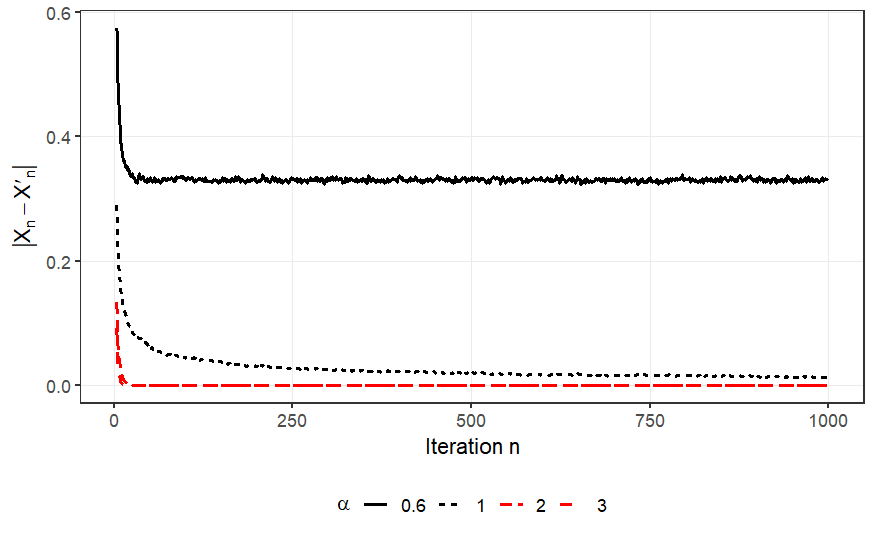
\includegraphics[width=0.7\linewidth]{images/randomlogmap_CRN}
	\caption{The simulated expected value of $|X_n-X'_n|$ where $X_n,X'_n$ are random logistic maps and CRN is applied ($X_0=0.5,X'_0=0.125$). For all $\alpha>1/2$, the chain converges in distribution. For $\alpha\geq 2$, the chain is geometrically ergodic. The CRN
		estimate uses the mean of $10 000$ simulations.}
	\label{fig:randomlogmapcrn}
\end{figure}
\begin{lemma}\label{lem:ranlogmap}
	CRN is an optimal coupling on the first iteration of the random logistic map when $k$ is QAC. 
	\begin{proof}
		Since $4X_{n-1}(1-X_{n-1})> 0$ w.p. 1, the function $4\beta_n X_{n-1}(1-X_{n-1})$ is increasing with respect to $\beta_n$. By Proposition \ref{prop:incr1}, CRN is an optimal coupling on the first iteration of the Markov chain when $k$ is QAC. 
	\end{proof}
\end{lemma}

%Note that while CRN is an optimal coupling for a 1-step random logistic map, it is not an optimal coupling for a multi-step random logistic map since $X_n$ is not an increasing function of $X_{n-1}$. For the optimal coupling of a 2-step random logistic map see Section \ref{subsec:ranlogmap2}. 
%\begin{numexmp}[Case when CRN is not the optimal coupling for a two step random logistic map]\label{numex:ranlogmap}
%	
%	Suppose that $X_0=\frac{1}{2}$ and $X'_0=\frac{1}{4}$. Then 
%	\begin{align*}
%		X_2&=4B_2B_1(1-B_1) &
%		X'_2&=3B'_2B'_1(1-0.75B'_1)
%	\end{align*}
%	CRN is the optimal coupling for $B_2$ since the $X_2,X'_2$ is always an increasing function of $B_2$. However, CRN is not the optimal coupling of $B_1$ and $B'_1$. 
%	
%	First note that over the interval $B_1,B'_1\in[0,1/2]$, $X_2,X'_2$ are increasing functions of $B_1,B'_1$. Over the interval $B_1,B'_1\in[2/3,1]$, $X_2,X'_2$ are decreasing functions of $B_1,B'_1$.  Over the interval $B_1,B'_1\in(1/2,2/3)$, $X_2,X'_2$ are decreasing and increasing functions of $B_1,B'_1$, respectively. Thus for $B_2$, $A=[0,1/2]\cup [2/3,1]$ where $A$ is defined in Theorem \ref{thm:iff}.
%	
%	Define $B_n\sim Beta(2,1)$, then $F_{B}(A)=[0,1/4]\cup [4/9,1]$. Define $U\sim \unif(0,1)$, $B_1=F^{-1}_B(U)$ and $B'_1=F^{-1}_B(V)$ where $V$ is defined as follows.
%	\begin{equation}\label{eq:ranlogmapV}
%		V=
%		\begin{cases}
%			U & \text{if } U\in [0,1/4]\cup [4/9,1]\\
%			\frac{1}{2}+\frac{4}{9}-U & \text{if } U\in (1/4,4/9)
%		\end{cases}
%	\end{equation}
%	The above joint distribution setup is based on Equation \ref{eq:Vstar}. Figure \ref{fig:randomlogmapcrnvsmin} provides the simulated expected distances of $E[(X_2-Y_2)^2]$ where the bottom line represents the expected distribution where $B_1,B'_1$ are simulated based on the joint distribution summarized above. The top line is the simulated expected distance when CRN is applied.
%\end{numexmp}
%\begin{figure}
%	\centering
%	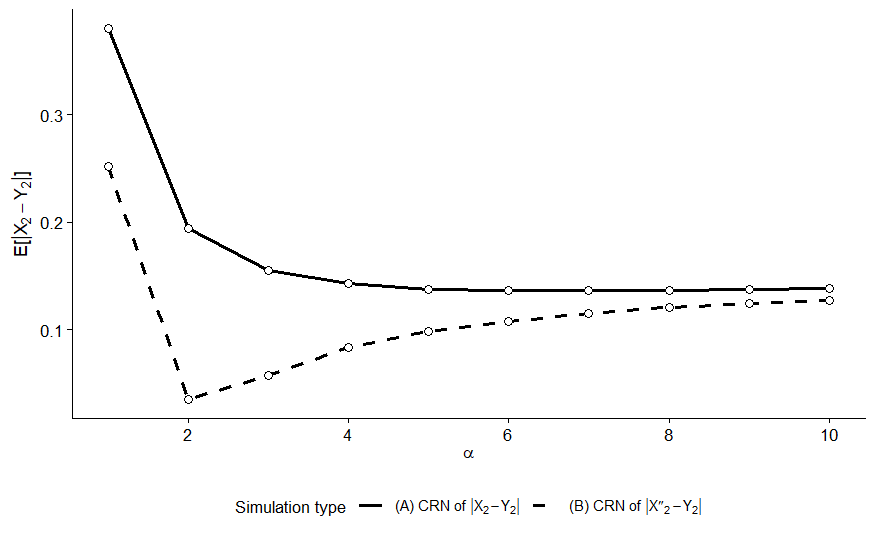
\includegraphics[width=0.7\linewidth]{images/randomlogmap_CRNvsMin}
%	\caption{Comparison of $E[(X_2-X'_2)^2]$ when the joint distribution of $J(B_1,B'_1)$ is the joint distrbution outlined in Equation \ref{eq:ranlogmapV} vs CRN. $B_i\sim Beta(\alpha+1/2,\alpha-1/2)$, $i\in \{1,2\}$. $B_2=B'_2$. The expected distance is based on $10^6$ simulations. }
%	\label{fig:randomlogmapcrnvsmin}
%\end{figure}

\subsubsection{Zeno's walk}
\begin{example}[Zeno's walk]\label{ex:zeno}
	Let $\{X_n\}_{n\geq 1}\in \mathbb{R}$ be a Zeno's walk (\cite{localcont}). That is for i.i.d. $B_n\sim \bernoulli(r)$, 
	$X_n=B_n f^{+}(X_{n-1})+(1-B_n)f^{-}(X_{n-1})$ where,
	
	\noindent\begin{minipage}{.5\linewidth}
		\[ f^{+}(x)=\begin{cases} 
			x+1 & 0\leq x \\
			\frac{x}{2}+1 & -2\leq x\leq 0 \\
			x+2 & x\leq -2 
		\end{cases}
		\]
	\end{minipage}%
	\begin{minipage}{.5\linewidth}
		\[ f^{-}(x)=\begin{cases} 
			x-1 & x\leq 0 \\
			\frac{x}{2}-1 & 0\leq x\leq 2 \\
			x-2 & 2\leq x 
		\end{cases}
		\]
	\end{minipage}
\end{example}

See Figure \ref{fig:zenoswalk} for a graphical representation of $f^{+}(x)$ and $f^{-}(x)$.
\begin{figure}
	\centering
	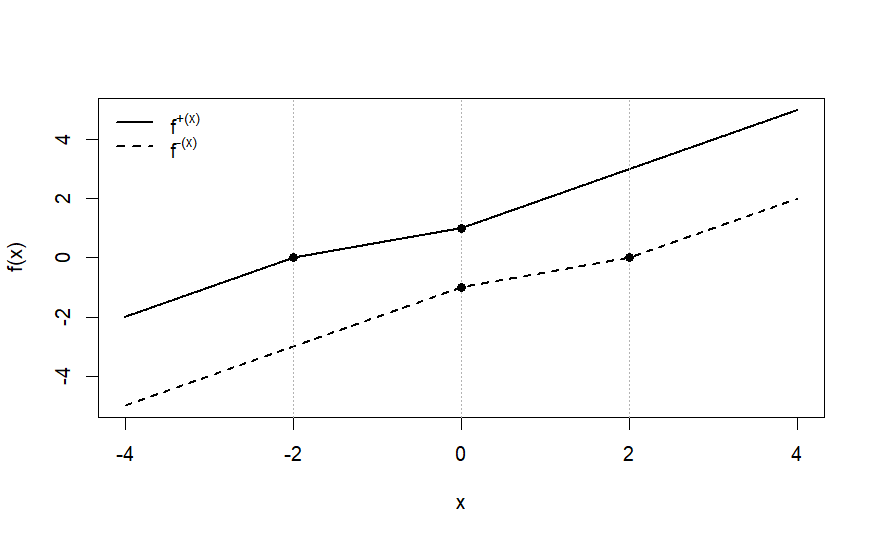
\includegraphics[width=0.7\linewidth]{images/zenos_walk}
	\caption{Graph of $f^{+}(x)$ and $f^{-}(x)$. It is clear from the graph that $f^{+}(x)-f^{-}(x)\geq 0$ for any $x\in \mathbb{R}$.}
	\label{fig:zenoswalk}
\end{figure}

Zeno's walk is locally contractive and geometrically ergodic if $\frac{1}{3}<r<\frac{2}{3}$ \cite{localcont}. In Lemma \ref{lem:zeno}, we show that CRN is the optimal coupling on the $n$th iteration of Zeno's walk.
\begin{lemma}\label{lem:zeno}
	CRN is an optimal coupling on the $n$th iteration of Zeno's walk when $k$ is QAC. 
	\begin{proof}
		First we show that CRN is an optimal coupling on the first iteration.
		
		We can re-write $X_n=f^{-}(X_{n-1}) + B_n (f^{+}(X_{n-1})-f^{-}(X_{n-1}))$.
		Note that $f^{+}(x)-f^{-}(x)>0$ for all $x\in\mathbb{R}$ (this is clear from Figure \ref{fig:zenoswalk}).%: 
%		\[ f^{+}(x)-f^{-}(x)=\begin{cases} 
%			x+2-(x-1)& x\leq -2 \\
%			\frac{x}{2}+1 - (x-1) & -2\leq x\leq 0 \\
%			x+1-(\frac{x}{2}-1) & 0\leq x\leq 2 \\
%			x+1-(x-2) & 2\leq x 
%		\end{cases}
%%		=\begin{cases} 
%%			3& x\leq -2 \\
%%			-\frac{x}{2}+2 & -2\leq x\leq 0 \\
%%			\frac{x}{2}+2 & 0\leq x\leq 2 \\
%%			3 & 2\leq x 
%%		\end{cases}
%		\geq\begin{cases} 
%			3& x\leq -2 \\
%			2 & -2\leq x\leq 2 \\
%			3 & 2\leq x 
%		\end{cases}
%		\]
		This means that for any $X_{n-1}\in \mathbb{R}$, the function $X_n=f^{-}(X_{n-1}) + B_n (f^{+}(X_{n-1})-f^{-}(X_{n-1}))$ is an increasing function of $B_n$ and so by Proposition \ref{prop:incr1},  for $k$ QAC, CRN is an optimal coupling on the first iteration of Zeno's walk.
		
		Next, since $f^{+}(x), f^{-}(x)$ are increasing functions of $x$ and $B_n,1-B_n\geq 0$, the function $B_n f^{+}(x)+(1-B_n)f^{-}(x)$ is an increasing function of $x$ and so, by Theorem \ref{thm:crnmc} CRN is the optimal coupling for the $n$th iteration of the Markov chain.   
	\end{proof}
\end{lemma}

%Figure \ref{fig:zenocrn} graphs the expected distance between two copies of the Zeno walk, $X_n,X'_n$ with initial values $X_0=0,X'_0=100$ when CRN is applied. By Lemma \ref{lem:zeno}, this is also the simulated estimate of the Wasserstein distance. Further, by Section 7.2 of \cite{localcont}, if $r\leq 1/3$ the process does not converge, which is confirmed by Figure \ref{fig:zenocrn} where the black lines ($r=0.1,1/3$) are the non-converging sequences.

Figure \ref{fig:zenocrn} displays the expected distance using CRN between two copies of the Zeno walk, $X_n$ and $X'_n$, initialized at $X_0 = 0$ and $X'_0 = 100$, respectively. By Lemma \ref{lem:zeno}, this is the unbiased estimate of the Wasserstein distance.

Moreover, Section 7.2 of \cite{localcont} asserts that the process fails to converge whenever $r \leq 1/3$. This theoretical result is reflected in Figure \ref{fig:zenocrn}: the black curves (corresponding to $r = 0.1$ and $r = 1/3$) are non-convergent, whereas the red curve (corresponding to $r = 0.5$) converges.

\begin{figure}
	\centering
	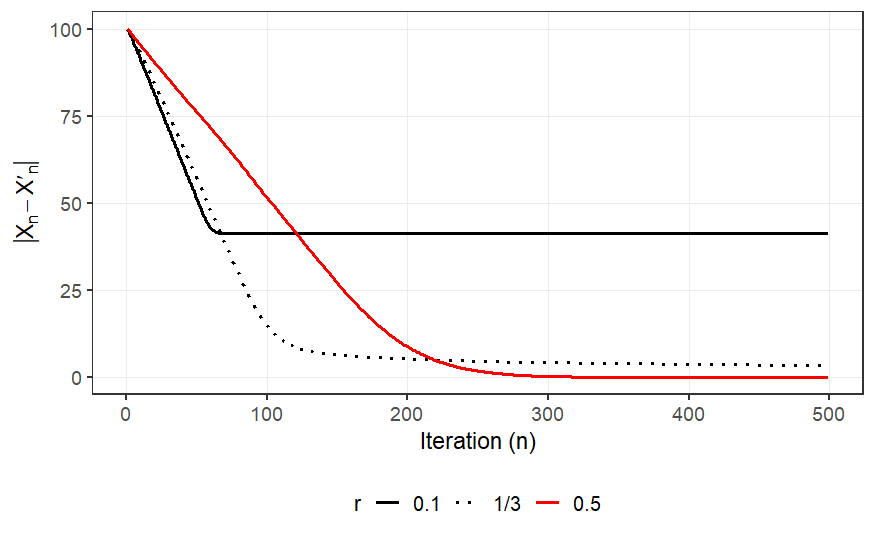
\includegraphics[width=0.7\linewidth]{images/zeno_CRN}
	\caption{The simulated expected value of $|X_n-X'_n|$ where $X_n,X'_n$ follow Zeno's walk and are simulated using CRN. The CRN
		estimate uses the mean of $1000$ simulations. $X_0=0,X'_0=100$. Since CRN is an optimal coupling (Lemma \ref{lem:zeno}), the simulations are unbiased estimates of the actual convergence rates.}
	\label{fig:zenocrn}
\end{figure}

\subsubsection{Autoregressive normal process in $\mathbb{R}^q$}
\begin{example}[Autoregressive normal process in $\mathbb{R}^q$]\label{ex:arnormdep}
	The random vector $\{\vecx_n\}_{n\geq 1}\in \mathbb{R}^q$ is an autoregressive normal process if for matrix $A$ and random vector $\vec{\theta}_n\sim N(\vec{0}_q,\Sigma_q^2)$. %($\Sigma_d^2$ is a positive semi-definite matrix)
	$$\vecx_{n}=A\vecx_{n-1}+\vec{\theta}_n$$
\end{example}

Theorem 4.13 of \cite{sixta} shows, using a CRN joint coupling (see Section \ref{subsec:contractioncond} for an explanation of the connection between contraction rates and CRN), that the AR process is geometrically ergodic when the maximum eigenvalue of $A$ is less than 1. If $A$ has only positive entries, then by Lemma \ref{lem:arnormdepnstep} below, we show that CRN is an optimal coupling for the $n$th iteration of the Markov chain.

%\begin{lemma}\label{lem:arnormdep1step}
%	CRN is an optimal coupling of the $\ell^p-$norm Wasserstein distance for the first iteration of the autoregressive normal process in $\mathbb{R}^q$. 
%	\begin{align*}
%		W_{||\cdot||_p,p}(\mathcal{L}(\vecx_1), \mathcal{L}(\vec{Y}_{1}))^{1/p}=
%		E[||A\vecx_{0}+\vec{\theta}_1-(A\vec{Y}_{0}+\vec{\theta}_1)||_p^p]^{1/p}
%	\end{align*}
%	\begin{proof}
%		For any fixed $i\in\{1,\ldots,q\}$ the coordinate $X_{i}=(A\vec{X}_{0})_{i}+\theta_{i}$ is an increasing function of $\theta_{i}$. So, by Theorem \ref{thm:rdrp}, CRN is an optimal coupling for the first iteration of the autoregressive normal process in $\mathbb{R}^q$.
%	\end{proof}
%\end{lemma}

	\begin{lemma}\label{lem:arnormdepnstep}
		 CRN is an optimal coupling for the first iteration of the autoregressive normal process in $\mathbb{R}^q$.
		 If $A$ has only positive entries, then CRN is an optimal coupling for the $n$th iteration of the autoregressive normal process in $\mathbb{R}^q$. 
		\begin{align}\label{eq:arnormdepnstep}
			W_{||\cdot||_p,p}(\mathcal{L}(\vecx_n), \mathcal{L}(\vec{Y}_{n}))=
			E[||f_n(\Theta_n,\vec{x}_{0})-(f_n(\Theta_n,\vec{y}_{0}))||_p^p]^{1/p}
		\end{align}
		Further, if the maximum eigenvalue of $A$ is less than 1, $||\vec{X}_n-\vec{Y}_{n}||_p\to 0$ w.p. 1 when generated by CRN.
	\end{lemma}
	\begin{proof}
		
		\underline{CRN is the optimal coupling at the first iteration:} For any fixed $i\in\{1,\ldots,q\}$ the coordinate $X_{i}=(A\vec{X}_{0})_{i}+\theta_{i}$ is an increasing function of $\theta_{i}$. So, by Theorem \ref{thm:rdrp}, CRN is an optimal coupling for the first iteration of the autoregressive normal process in $\mathbb{R}^q$.
		
	\underline{CRN is the optimal coupling at the $n$th iteration:}
		Fix $i,l\in \{1,\ldots q\}$ and $x_i<x'_i$. Since $a_{lj}\geq 0$ by assumption, $$f^{(l)}(\vec{\theta},(\vec{x}_{-i},x_i))= a_{li}x_i +\sum_{j\neq i}a_{lj}x_j +\theta_l\leq a_{li}x'_i +\sum_{j\neq i}a_{lj}x_j +\theta_l= f^{(l)}(\vec{\theta},(\vec{x}_{-i},x'_i))$$ Since and $i,l$ were arbitrary, $A\vec{x}+\vec{\theta}$ is coordinate-wise monotone in $\vec{x}$. 
		By Theorem \ref{thm:crnmc} CRN is an optimal coupling on the $n$th iteration of the autoregressive normal process in $\mathbb{R}^q$ and equation \ref{eq:arnormdepnstep} holds.  
		Finally, Theorem 4.23 of \cite{sixta} shows that if the maximum eigenvalue of $A$ is less than 1, then the process is geometrically ergodic, so by Corollary \ref{cor:convwp1}, $||\vec{X}_n- \vec{Y}_{n}||_p^p\to 0$ w.p. 1 when generated by CRN.
	\end{proof}

\subsubsection{Bayesian location model Gibbs sampler}
\begin{example}[Bayesian location model Gibbs sampler]\label{ex:locmodel}
	Suppose that we are given data points $Y_1,\ldots, Y_J \sim N(\mu, \tau^{-1})$ where $\mu, \tau^{-1}$ are unknown and $J\geq 3$. Let $\mu, \tau^{-1}$ have flat priors on $\mathbb{R}$ and $\mathbb{R}_+$. The Gibbs algorithm is based on the marginal posterior distributions of $\mu, \tin$ and the conditional distributions are defined as follows.
	
	\begin{itemize}
		\item $\mu_{n+1} = \bar{y} + Z_{n+1}/\sqrt{J \tau_{n}}$
		\item $\tau^{-1}_{n+1} = \frac{\frac{S}{2}+\frac{J}{2}(\bar{y}-\mu_{n+1})^2}{G_{n+1}}$
	\end{itemize}
	Where $Z_{n}\sim N(0,1)$ and $G_{n}\sim \Gamma(\frac{J+2}{2},1)$ are independent and $S=\sum_{i=1}^J (y_i-\bar{y})^2$. $\Gamma(\alpha, \beta)$ represents the gamma distribution, $\Gamma^{-1}(\alpha, \beta)$ represents the inverse gamma distribution where $\alpha$ and $\beta$ represent the shape and scale, respectively.
	
	The variable $\tau^{-1}$ can be written as a random-coefficient auto-regressive process $\tinv_{n}=H_nG_n\tinv_{n-1}+G_n$
	where $H_n\sim \Gamma\left(\frac{1}{2}, \frac{S}{2}\right)$ and $G_n\sim \Gamma^{-1}\left(\frac{J+2}{2}, \frac{S}{2}\right)$.
\end{example}

Theorem 6 of \cite{oneshot} and Theorem 4.14 of \cite{sixta} show, via a CRN coupling (see Section \ref{subsec:contractioncond} for the relationship between contraction rates and CRN), that the Gibbs sampler for the Bayesian location model has contraction rate of $\frac{1}{J}$. 
	\begin{lemma}\label{lem:locmodel}
		CRN is an optimal coupling on the $n$th iteration of the Bayesian location model Gibbs sampler when $k$ is QAC. That is for $\vec{\theta}_n=(H_n,G_n)$,
		\begin{align}\label{eq:locmodel}
			W_{k}(\mathcal{L}(\tau^{-1}_{n}), \mathcal{L}(\tau^{-1'}_{n}))=
			E[k(f_n(\Theta_n,\tau^{-1}_{0}),f_n(\Theta_n,\tau^{-1'}_{0}) )]
		\end{align}
		Further, $k(\tinv_{n}, \tau^{-1'}_{n})\to 0$ w.p. 1 when generated by CRN.
		\begin{proof}
			Note first that $H_n, G_n,\tau_{n-1}^{-1}\geq 0$. 
			For any $H_n=h, \tau_{n-1}^{-1}=\tinv$, the function $\tinv_{n}=hG_n\tinv+G_n$ is increasing with respect to $G_n$. 
			For any $G_1=g, \tau_{n-1}^{-1}=\tinv$, the function $\tinv_{1}=H_ng\tin+g$ is increasing with respect to $H_n$. 
			For any $H_n=h, G_n=g$, the function $\tinv_{1}=hg\tin_{n-1}+g$ is increasing with respect to $\tin_{n-1}$. Thus, $f$ is coordinate-wise monotone in terms of $(H_n, G_n)$ and $\tau^{-1}_n$.
			
			So by Theorem \ref{thm:crnmc}, CRN is an optimal coupling on the $n$th iteration of the Bayesian location model Gibbs sampler when $k$ a QAC norm and equation \ref{eq:locmodel} follows.
			
			Finally, Theorem 4.14 of \cite{sixta} shows that the process is geometrically ergodic. By Corollary \ref{cor:convwp1}, $k(\tinv_{n}, \tau^{-1'}_{n})\to 0$ w.p. 1 when generated by CRN.
		\end{proof}
	\end{lemma}

%\subsubsection{Gibbs sampler related to the James Stein estimator}
%\begin{example}[A model related to James-Stein estimators]\label{ex:stein}
%	
%	Suppose that we have observed data $Y\in \mathbb{R}^q$ such that each $Y_i$ is normally distributed according to a unique mean $\theta_i$,
%	$Y_i\sim N(\theta_i,V)$.
%	Suppose that $V>0$ is known and that $\theta_i\sim N(\mu,A)$ ($\theta_i$'s are i.i.d.), where $\mu$ has a flat prior and $A\sim IG(\alpha,\beta)$.
%	 The conditional distributions are defined as follows.
%	 \begin{itemize}
%	 	\item $\theta_{n,i}|\mu_{n-1}, A_{n-1},Y \sim N(\frac{Y_{i}A_{n-1}+\mu_{n-1} V}{A_{n-1}+V},\frac{VA_{n-1}}{V+A_{n-1}})$
%	 	\item $\mu_n| \vec{\theta}_{n},A_{n-1},Y \sim N(\bar{\theta}_{n},A_{n-1}/q)$ where $\bar{\theta}_n=\frac{1}{q}\sum_{i=1}^q \theta_{n,i}$
%	 	\item $A_n|\vec{\theta}_{n},\mu_{n},Y \sim IG\left(\alpha+ \frac{q-1}{2},\frac{\sum_{i=1}^q(\theta_{n,i}-\mu_{n})^2}{2}+\beta\right)$
%	 \end{itemize}
%	The joint posterior density function of $\vec{\theta},\mu,A\mid Y$ is proportional to the following equation,
%	\begin{align}\label{eqn:jsteinG}
%		g(\vec{\theta},\mu,A\mid Y) = f_{IG}(A\mid \alpha, \beta) \times \prod_{i=1}^q f_N(Y_i\mid \theta_i, V)  \times \prod_{i=1}^q f_N(\theta_i \mid \mu, A)
%	\end{align}		
%\end{example}
%\paragraph{The Gibbs sampler for a model related to James-Stein estimators.} 
%
%Algorithm \ref{alg:stein} shows how to apply a Gibbs sampler on this example.
%\begin{algorithm}\label{alg:stein}
%	\caption{The Gibbs sampler algorithm for a model related to James-Stein estimators.}\label{alg:stein}
%	\begin{algorithmic}
%		\State Initialize $(\vec{\theta}_0,\mu_0,A_0)$
%		\For{$n = 1, \ldots, N$}
%		\State For each $i\in 1,\ldots, q$, generate $\theta_{n,i}|\mu_{n-1}, A_{n-1},Y \sim N(\frac{Y_{i}A_{n-1}+\mu_{n-1} V}{A_{n-1}+V},\frac{VA_{n-1}}{V+A_{n-1}})$
%		\State Generate $\mu_n| \vec{\theta}_{n},A_{n-1},Y \sim N(\bar{\theta}_{n},A_{n-1}/q)$ where $\bar{\theta}_n=\frac{1}{q}\sum_{i=1}^q \theta_{n,i}$
%		\State Generate $A_n|\vec{\theta}_{n},\mu_{n},Y \sim IG\left(\alpha+ \frac{q-1}{2},\frac{\sum_{i=1}^q(\theta_{n,i}-\mu_{n})^2}{2}+\beta\right)$
%		\EndFor
%	\end{algorithmic}
%\end{algorithm}


\subsubsection{Linear ARCH process}
\begin{example}[Linear ARCH process]\label{ex:lineararch}
	Let $\{X_n\}_{n\geq 1}\in \mathbb{R}$ be a linear ARCH process. Then for i.i.d. $\theta_n$
	$$X_n = (\beta_0 +\beta_1 X_{n-1})\theta_n$$
\end{example}

We show that for the linear ARCH process, if $X_n\geq 0$ for all $n\in\mathbb{N}$, CRN is the joint coupling that generates the Wasserstein distance for iteration $n\geq 1$ and that if the process is geometrically ergodic, then the $\ell^p$ distance converges to 0 w.p. 1.
\begin{lemma}\label{lem:lineararch}
	Suppose that $\beta_0,\beta_1>0$ and $\theta_n>0$ a.s., then CRN is an optimal coupling on the $n$th iteration of the linear ARCH process when $k$ is QAC. 
	\begin{align}\label{eq:lineararch}
		W_{k}(\mathcal{L}(X_{n}), \mathcal{L}(Y_{n}))=
		E[k(f_n(\Theta_n, x_0),f_n(\Theta_n, y_0))]
	\end{align}
	Further, if $\beta_1 E[|\theta_0|]<1$, $k(X_{n},Y_{n})\to 0$ w.p. 1 when generated by CRN.
	
	\begin{proof}
		Since $(\beta_0 +\beta_1 X_{n-1})>0$ w.p. 1, $X_n=f(\theta_n,X_{n-1})$ is always an increasing function of $\theta_n$. Since $\beta_1\theta_n>0$ w.p. 1, $f(\theta_n,X_{n-1})$ is always an increasing function of $X_{n-1}$. So by Theorem \ref{thm:crnmc}, CRN is an optimal coupling on the $n$th iteration of the linear ARCH process when $k$ is QAC. 
		Finally if $\beta_1 E[|\theta_0|]<1$, then the process is geometrically ergodic (Theorem 5.1 of \cite{sixta}), so by Corollary \ref{cor:convwp1}, $k(X_{n},Y_{n})\to 0$ w.p. 1 when generated using CRN. 
	\end{proof}
\end{lemma}

\section{When monotone conditions are not satisfied}

Monotonicity is important when establishing the optimal coupling between two random variables, because it orders the function with regard to what is relevant: the distance between $f(\theta,x)$ and $f(\theta,y)$ as a function of $U$ where $\theta=f^{-1}_{\theta}(U)$. However, sometimes $f$ is not monotone. In such cases we ask ourselves, is CRN the optimal coupling? Probably not. So, how could we generate a coupling that has lower expected distance? If we can propose an equimeasurable rearrangement of $f$ w.r.t $U$, $f^*$, that is monotone, then CRN applied to the proposed $f^*$ would generate the optimal coupling.

In the following section, we propose two equimeasurable transformations $g:[0,1]\to [0,1]$ and $h:[0,1]\times \{0,1\}\to [0,1]$ that, when used correctly, generate monotone functions and consequently lower expected distances when simulated using CRN. 
%\begin{definition}[Equimeasurable function of $f(U)$]
%	Let $f:[0,1]\to \mathbb{R}$ and $U\sim \unif(0,1)$. $f^*$ is an equimeasurable function of $f(U)$ if $\mathcal{L}(f(U))=\mathcal{L}(f^*(U))$.
%\end{definition} 

\subsection{Equimeasurable functions}
`Equimeasurable' when used within the context of CRN was discussed as early as 1934 \cite{inequalities}. The equimeasurable functions, however, were limited to the quantile transformation of $U\sim \unif(0,1)$, which is described in Section \ref{sec:invdf}. %In Section 10.12 of \cite{inequalities}, it was shown that the covariance maximizing joint distribution is the equimeasurable monotone rearrangement or more specifically the inverse CDF of a uniform random variable in $\mathbb{R}$. In \cite{rearrangefunc}, similar results were generated for a random variable in $\mathbb{R}^q$. 
Equimeasurable rearrangements were also defined in Chapter 1 of \cite{villani}, and \cite{quantile1}, but was again only defined in terms of quantile functions. 

While the quantile function is an optimal transformation, in the problem setup with IRFs we do not know the CDF of $X$, but only know that $X=f(\theta,x)$ and that $\theta=F^{-1}_{\theta}(U)$ for known $F_{\theta}$. Thus we're interested in generating an equimeasurable monotone rearrangment of $f(F^{-1}_{\theta}(U),x)$ with respect to $U$ by creating a mapping $g:[0,1]\to [0,1]$ such that $f(F^{-1}_{\theta}(g(U)),x)$ is a monotone function of $U$ and $\mathcal{L}(f(F^{-1}_{\theta}(g(U)),x))=\mathcal{L}(f(F^{-1}_{\theta}(U),x))$. %, which by extension is the inverse CDF of $X$ a.s. % for functions in $\mathbb{R}^q$ (Section 10.12 of \cite{inequalities}) and \cite{quantile1,villani}, but was again restricted to inverse CDF functions. 

In this section we study equimeasurable functions as transformations on the random variable $U$ that preserve the measure of $U$ (see Definition \ref{def:equimeasurable}). This is similar to the approach taken in \cite{equimeasurable, equimeasurable2}, which studied generating lower bounds on eigenvalues using rearrangements of the eigenfunctions. 

\begin{definition}[Equimeasurable function of $f(U)$]\label{def:equimeasurable}
	Let $f:[0,1]\to \mathbb{R}$ and $U\sim \unif(0,1)$. $f^*$ is an equimeasurable function of $f$ if $\mathcal{L}(f(U))=\mathcal{L}(f^*(U))$.
\end{definition} 

An equimeasurable function $f^*$ is specific to the function $f$ and the random variable $U$. In this paper we restrict our definition to $U\sim \unif(0,1)$. 

%\subsection{}
The following are two function transformations that can be applied to $U$. We can then use these transformations to generate monotone equimeasurable transformations of our random function. %Finally, when two random variables are redefined in terms of montone equimeasurable transforms, CRN is then the optimal joint distribution.

If the values of a function are flipped over an interval $(a,b)\in[0,1]$, Lemma \ref{lem:intflip} states that this is an equimeasurable function.

Lemma \ref{lem:intmerge} states that if I partition an interval into two parts $(a,b)=(a,t)\cup(t,b)$ then I can replace the interval $(a,b)$ with $(a,t)$ with probability $\frac{t-a}{b-a}$ and replace it with $(t,b)$ with probability $\frac{b-t}{b-a}$, hence `merging' two intervals. 
 

%In this section we apply the idea of equimeasurable functions to iterated random functions. In particular, if we can define a function $g:[0,1]\to[0,1]$ such that $g(U)\sim \unif(0,1)$ whenever $U\sim \unif(0,1)$, then $P(f(F^{-1}_{\theta}(g(U)),x)\leq t)=P(f(F^{-1}_{\theta}(U),x)\leq t)$ for $t\in \mathbb{R}$ and so, $f^*=f\cdot g$ is an equimeasurable function of $f$.

\begin{lemma}[Interval flip]\label{lem:intflip}
	Let $(a,b)\subset [0,1]$, $U\sim\unif(0,1)$, and the function $g$ to be 
	\begin{equation}\label{eq:g}
		g(U)=
		\begin{cases}
			U & \text{if } U\notin (a,b)\\
			%F_{X_{B_i}}^{-1}(1-F_{X_{B_i}}(U)) & \text{if } U\in F_{\theta}(B_i)=(a_i,b_i)
			a+b-U & \text{if } U\in (a,b)
		\end{cases}
	\end{equation}
	 Then $\mathcal{L}(f(U))=\mathcal{L}(f(g(U)))$. %$$P(f(F^{-1}_{\theta}(g(U)),x)\leq t)=P(f(F^{-1}_{\theta}(U),x)\leq t)$$ $g(U)\sim\unif(0,1)$.
	The proof can be found in Section \ref{sec:intflip}.
\end{lemma} 

%\begin{algorithm}
%		\caption{Function $h(U,\xi)$: Merging two intervals together, $(a,t)$ and $(t,b)$}\label{alg:mergeint}
%	\begin{algorithmic}
%	\State Simulate $U\sim \unif(0,1)$ and $\xi\sim \mathrm{Bernoulli}(\frac{t-a}{b-a})$
%		\If{$U\in (a,b)$}
%		%\State $B\sim \mathrm{Bernoulli}(\frac{t-a}{b-a})$
%		\If {$\xi=1$}
%		\State $h(U,1)\leftarrow\frac{U-a}{b-a}(t-a)+a$
%		\Else 
%		\State $h(U,0)\leftarrow\frac{U-a}{b-a}(b-t)+t$
%		\EndIf
%		\Else 
%		\State $h(U,\xi)=U$
%		\EndIf
%		\State \textbf{Return} $h(U,\xi)$
%	\end{algorithmic}
%\end{algorithm}
\begin{lemma}[Interval merge]\label{lem:intmerge}
	Let $(a,b)\subset [0,1]$, $t\in (a,b)$, $U\sim \unif (0,1)$ and the functions $h(U,\xi)$ be as follows for independent random variables $U\sim \unif (0,1)$ and $\xi\sim \mathrm{Bernoulli}(\frac{t-a}{b-a})$
	\begin{equation}\label{eq:h}
		h(U,\xi)=
		\begin{cases}
			\xi \left(\frac{t-a}{b-a}(U-a)+a\right) + (1-\xi) \left(\frac{b-t}{b-a}(U-a)+t\right) & \text{if } U\in (a,b)\\
			U & \text{if } U\notin (a,b)
		\end{cases}
	\end{equation}
	Then $\mathcal{L}(f(U))=\mathcal{L}(f(h(U,\xi)))$.
	The proof can be found in Section \ref{sec:intmerge}.
\end{lemma}

\subsection{Example}\label{subsec:ranlogmap2}

\begin{numexmp}[Random Logistics Map]\label{numex:ranlogmap}
We revisit Example \ref{ex:randomlogmap}, to prove by counterexample that CRN is not the optimal coupling for a two-step random logistic map, even though it is the optimal one step coupling. Suppose that the initial values of the random logistic map are 
$X_0=\frac{1}{2}$ and $Y_0=\frac{1}{8}$, then the second iteration of the functions are
\begin{align}\label{eq:x2y2}
	X_2&=4B_2B_1(1-B_1) &
	Y_2&=\frac{7}{4}B'_2B'_1\left(1-\frac{7}{16}B'_1\right)
\end{align} 

Recall $B_1,B_2\sim \beta(\alpha+1/2,\alpha-1/2)$. Denote $F_{\beta}$ to be the CDF of $\beta(\alpha+1/2,\alpha-1/2)$ so that $F_{\beta}^{-1}(U)\sim \beta(\alpha+1/2,\alpha-1/2)$. We can then re-write $X_2$ as follows where $U_1\sim \unif(0,1)$ and $U_1, B_2$ are independent,
\begin{align*}
	X_2(U_1,B_2)&=4B_2F^{-1}_{\beta}(U_1)(1-F^{-1}_{\beta}(U_1))
\end{align*} 
Observe that for any $B_2$, $X_2$ is an increasing function of $U_1$ when $U_1\in [0,F_{\beta}(0.5)]$ and a decreasing function of $U_1$ when $U_1\in [F_{\beta}(0.5),1]$. We will construct an equimeasurable transform of $X_2(U_1, B_2)$, $X''_2(U_1, B_2, \xi)$, that is monotone in $U_1$ for $\xi\in \{0,1\}$.  To do so, we first generate an equimeasurable function, $X'_2(U_1,B_2)=X(g(U_1),B_2)$, that is increasing over $U_1\in (F_{\beta}(0.5),1]$ where $g:[0,1]\to[0,1]$ is defined as follows,
 
\begin{equation}\label{eq:g}
	g(U)=
	\begin{cases}
		U & \text{if } U\in [0,F_{\beta}(0.5)]\\
		%F_{X_{B_i}}^{-1}(1-F_{X_{B_i}}(U)) & \text{if } U\in F_{\theta}(B_i)=(a_i,b_i)
		1+F_{\beta}(0.5)-U & \text{if }U\in (F_{\beta}(0.5),1]\\
	\end{cases}
\end{equation}
By Lemma \ref{lem:intflip}, $\mathcal{L}(X'_2)=\mathcal{L}(X_2)$. 

The interval flip is easiest to visualize in Figure \ref{fig:ranlogmapflip}.  In graph (A), when $U_1<F_{\beta}(0.5)\approx 0.288$ ($B_1<0.5$), $X_2(U_1,B_2)=X'_2(U_1,B_2)$, however when $U_1>F_{\beta}(0.5)$ ($B_1>0.5$), $X_2(U_1,B_2)$ is represented by the black line while the transform $X'_2(U_1,B_2)$ is represented by the red line. Note that the transform  $X'_2(U_1,B_2)$ is increasing when $U_1>F_{\beta}(0.5)$.

\begin{figure}
	\centering
	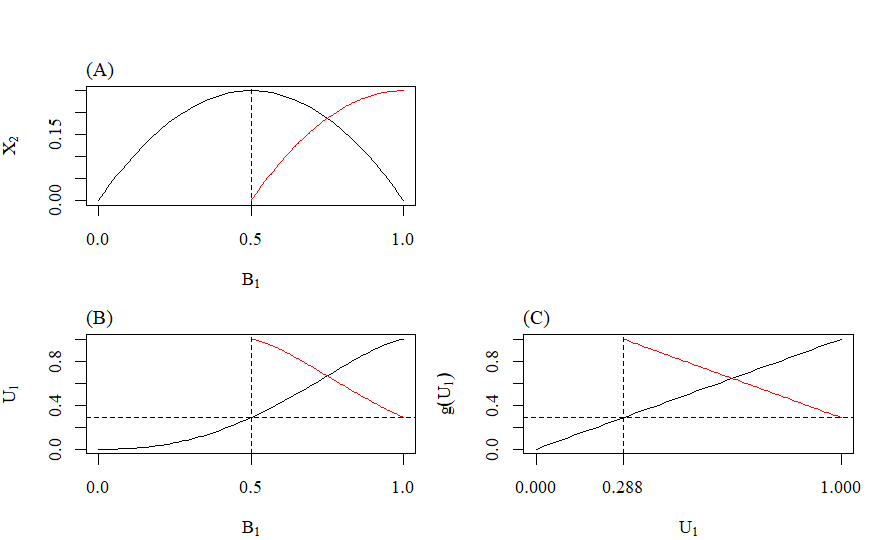
\includegraphics[width=1\linewidth]{images/ranlogmap_flip}
	\caption{Set $\alpha=2$ so that $B_1\sim \beta(2.5,1.5)$ and $F_{\beta}(0.5)= 0.288$. Set $B_2=1$ (its value is of little importance since it does not affect whether $B_1$ is increasing or not). In graph (A), the black line denotes $X_2(U_1,1)$ and the red line denotes $X'_2(U_1,1)$ when it is not equal to $X_2(U_1,1)$. 
	Graph (C) represents the transformation $g(U_1)$ in red compared to the identity function. Graph (B) then imposes the flip that was applied by $g$ onto the values of $B_1$. Graph (A) shows the effect of the flip, $g$, through $B_1$ onto the value of $X_2$.}
	\label{fig:ranlogmapflip}
\end{figure}

The transform $X'_2(U_1, B_2)$ is increasing over $U_1\in [0,F_{\beta}(0.5))$ and $U_1\in (F_{\beta}(0.5),1]$. However, it is not monotonically increasing. To generate an equimeasurable map that is monotonically increasing with respect to $U$, we use Lemma \ref{lem:intmerge} and introduce the auxiliary random variable $\xi$. 

Let $(a,b)=[0,1]$ and $t=F_{\beta}(0.5)$. Then $X''_2(U_1,B_2,\xi)=X_2(g(h(U_1,\xi)),B_2)$ where $h(U_1,\xi)$ is generated according to Equation \ref{eq:h} is an equimeasurable function of $U$ (Lemma \ref{lem:intmerge}). To summarize, $X''_2$ can be defined as follows for $\xi\sim \text{Bernoulli}(F_{\beta}(0.5))$
\begin{equation}\label{eq:X2gh}
	X''_2(U_1,B_2,\xi)=
	\begin{cases}
		4B_2 F_{\beta}^{-1}(1-U_1(1-F_{\beta}(0.5)))[1-F_{\beta}^{-1}(1-U_1(1-F_{\beta}(0.5)))] & \text{if } \xi=0\\
		4B_2 F_{\beta}^{-1}(F_{\beta}(0.5) U_1) [1-F_{\beta}^{-1}(F_{\beta}(0.5) U_1)] & \text{if } \xi=1\\
	\end{cases}
\end{equation}
  Summarizing, Lemmas \ref{lem:intmerge} and \ref{lem:intflip} imply that  $X''_2(U_1,B_2,\xi)$ is an equimeasurable transform of $X_{2}(U_1,B_2)$. Figure \ref{fig:ranlogmapdensities} (A) graphs the simulated density of $X_2(U_1,B_2)$ and $X''_2(U_1,B_2,\xi)$, which visually shows that the  densities are equal. 

\begin{figure}
	\centering
	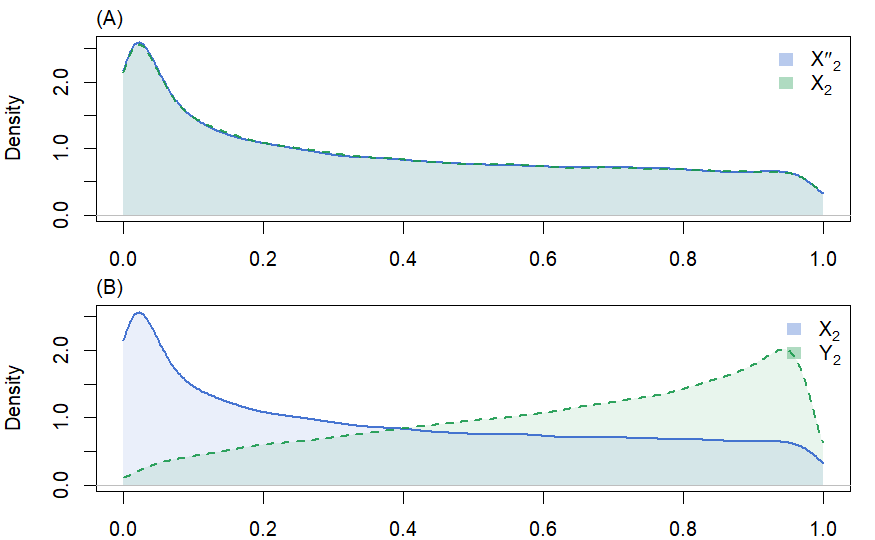
\includegraphics[width=0.7\linewidth]{images/ranlogmap_densities}
	\caption{(A): Simulated density of $X_2=4B_2B_1(1-B_1)$ and $X''_2(U_1,B_2,\xi)$ (see Equation \ref{eq:X2gh}). The random variables $B_i\sim Beta(1.5,0.5), i\in \{1,2\}$, $U_1\sim \unif(0,1)$, $\xi\sim \text{Bernoulli}(F_{\beta}(0.5))$ are independent. 
This shows that the random variable $X''_2$, which is based on the transformations $g$ and $h$ are indeed equimeasurable to $X_2$. (B): Comparison of the density of $X_2$ and $Y_2$
	}
	\label{fig:ranlogmapdensities}
\end{figure}

Finally, we want to show that CRN applied to $X_2(U_1,B_2)$ and $Y_2=(U'_1,B'_2)$ is not the optimal coupling since $X_2$ is not an increasing function with respect to $U_1$. To do this we've simulated using CRN $X''_2(U_1,B_2,\xi)$, which is equimeasurable to  $X_2(U_1,B_2)$, and $Y_2=(U'_1,B'_2)$, which is increasing with respect to $U_1'$ and $B_2'$. Figure \ref{fig:randomlogmapcrnvsmin} shows how the solid line, which is CRN applied to $|X_2(U_1,B_2)-Y_2(U_1,B_2)|$ has a larger expected distance compared to the transformed $|X''_2(U_1,B_2,\xi)-Y_2(F^{-1}_{\beta}(U_1),B_2)|$.

\begin{figure}
	\centering
	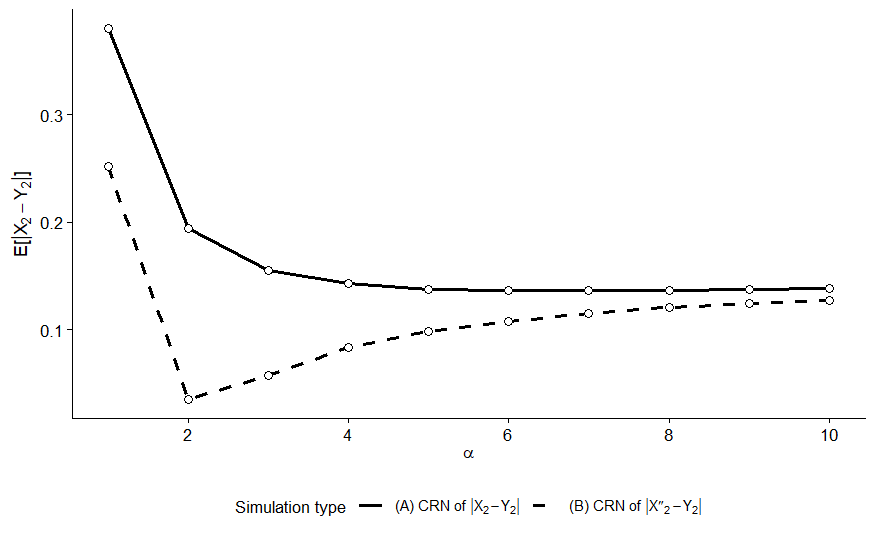
\includegraphics[width=0.7\linewidth]{images/randomlogmap_CRNvsMin}
	\caption{Line (A) represents the simulated expected distance of $|X_2(U_1,B_2)-Y_2(U_1,B_2)|$ ie. the expected distance when CRN is applied to the original function. Line (B) represents the simulated expected distance of $|X''_2(U_1,B_2,\xi)-Y_2(U_1,B_2)|$ ie. the expected distance when CRN is applied to the transformed $X''_2(U_1,B_2,\xi)$.}
	\label{fig:randomlogmapcrnvsmin}
\end{figure}

%Next we note that $Y_2$ is an increasing function of both $B_1$ and $B_2$ in $[0,1]$, so we will not modifying this equation.

%We show how the above transformation of $X''_2$ generates the optimal coupling with $Y_2$ in the following Lemma. 
%\begin{lemma}\label{lem:logregwass}
%	Let $X_2$ and $Y_2$ be defined as in Equation \ref{eq:x2y2} and $X''_2(U_1,\xi)=X_2(g(h(U_1,\xi)))$ where $g$ is defined as in Equation \ref{eq:g} and $h$ is defined as in algorithm \ref{alg:mergeint} where $(a,b)=[0,1]$ and $t=F_{\beta}(0.5)$. 
%	
%	The Wasserstein distance between $X_2,Y_2$ is equal to the distance between $Y_2$ and $X''_2$ when CRN is applied,  
%	$$W_p(X_2,Y_2)=E[k(X''_2(U_1,B_2,\xi),Y_2(U_1,B_2))]$$
%	
%	\begin{proof}
%		First note that $Y_2(U_1,B_2)=\frac{7}{4}B_2F_{\beta}^{-1}(U_1)\left(1-\frac{7}{16}F_{\beta}^{-1}(U_1)\right)$ is an increasing function of both $U_1\in[0,1]$ and $B_2\in [0,1]$. 
%		
%		Next note that 
%		$X_2=4B_2F_{\beta}^{-1}(g(h(U_1,\xi)))[1-F_{\beta}^{-1}(g(h(U_1,\xi)))] $ is an increasing function of $B_1$. 
%		
%		$X_2$ is an increasing function of $U_1$ when $\xi=0$: if $\xi=0$, then $h(U_1,0)\in (F_{\beta}(0.5),1)$ and $B_1=g(h(U_1,0))\in (0,0.5)$, which is an increasing function of $U_1$ as show in Figure \ref{fig:ranlogmapflip}(A).
%		
%		$X_2$ is an increasing function of $U_1$ when $\xi=1$: if $\xi=1$, then $h(U_1,0)\in (0,F_{\beta}(0.5))$ and $B_1=g(h(U_1,1))\in (0.5,1)$, which is an increasing function of $U_1$ as show in Figure \ref{fig:ranlogmapflip}(A).
%		\end{proof}
%\end{lemma}

\end{numexmp}

%\begin{numexmp}[Case when CRN is not the optimal coupling for a two step random logistic map]\label{numex:ranlogmap}
%	
%	Suppose that $X_0=\frac{1}{2}$ and $X'_0=\frac{1}{4}$. Then 
%	\begin{align*}
%		X_2&=4B_2B_1(1-B_1) &
%		X'_2&=3B'_2B'_1(1-0.75B'_1)
%	\end{align*}
%	CRN is the optimal coupling for $B_2$ since the $X_2,X'_2$ is always an increasing function of $B_2$. However, CRN is not the optimal coupling of $B_1$ and $B'_1$. 
%	
%	First note that over the interval $B_1,B'_1\in[0,1/2]$, $X_2,X'_2$ are increasing functions of $B_1,B'_1$. Over the interval $B_1,B'_1\in[2/3,1]$, $X_2,X'_2$ are decreasing functions of $B_1,B'_1$.  Over the interval $B_1,B'_1\in(1/2,2/3)$, $X_2,X'_2$ are decreasing and increasing functions of $B_1,B'_1$, respectively. Thus for $B_2$, $A=[0,1/2]\cup [2/3,1]$ where $A$ is defined in Theorem \ref{thm:iff}.
%	
%	Define $B_n\sim Beta(2,1)$, then $F_{B}(A)=[0,1/4]\cup [4/9,1]$. Define $U\sim \unif(0,1)$, $B_1=F^{-1}_B(U)$ and $B'_1=F^{-1}_B(V)$ where $V$ is defined as follows.
%	\begin{equation}\label{eq:ranlogmapV}
%		V=
%		\begin{cases}
%			U & \text{if } U\in [0,1/4]\cup [4/9,1]\\
%			\frac{1}{2}+\frac{4}{9}-U & \text{if } U\in (1/4,4/9)
%		\end{cases}
%	\end{equation}
%	The above joint distribution setup is based on Equation \ref{eq:Vstar}. Figure \ref{fig:randomlogmapcrnvsmin} provides the simulated expected distances of $E[(X_2-Y_2)^2]$ where the bottom line represents the expected distribution where $B_1,B'_1$ are simulated based on the joint distribution summarized above. The top line is the simulated expected distance when CRN is applied.
%\end{numexmp}
%\begin{figure}
%	\centering
%	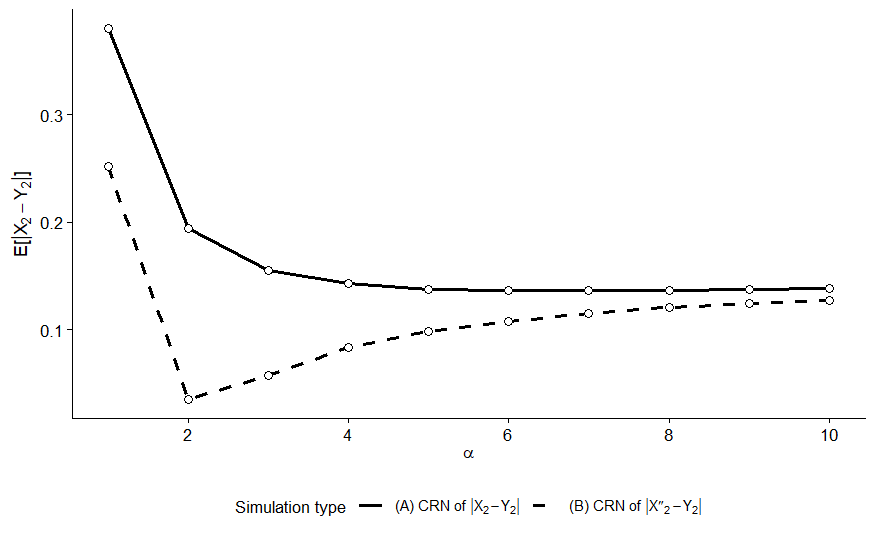
\includegraphics[width=0.7\linewidth]{images/randomlogmap_CRNvsMin}
%	\caption{Comparison of $E[(X_2-X'_2)^2]$ when the joint distribution of $J(B_1,B'_1)$ is the joint distrbution outlined in Equation \ref{eq:ranlogmapV} vs CRN. $B_i\sim Beta(\alpha+1/2,\alpha-1/2)$, $i\in \{1,2\}$. $B_2=B'_2$. The expected distance is based on $10^6$ simulations. }
%	\label{fig:randomlogmapcrnvsmin}
%\end{figure}

	
	\section{Connection between CRN and the backwards process}\label{subsec:backwardsprocess}
	\paragraph{Backwards process }
	
	The backwards process coupled with contraction conditions are commonly used to establish theorems that generate upper bounds on the Wasserstein distance between the distribution of a Markov chain and its corresponding stationary distribution (see \cite{iteratedranfunc,avcont,localcont}).
	
	The backward process, $\{\tilde{X}_n\}_{n\geq 1}$, which is not a Markov chain \cite{localcont} but tends to converge pointwise to a limit, is defined as follows,
	\begin{equation}\label{eq:backward}
		\tilde{X}_n = f(\theta_1,(f(\theta_{2},\ldots f(\theta_n,X_0)))
	\end{equation}
	The difference between the Markov chain and the backwards process is the order of $\theta_1,\theta_2,\ldots,\theta_n$ to generate the next iteration (Note the forward process, $X_n = f(\theta_n,(f(\theta_{n-1},\ldots f(\theta_1,X_0)))$, compared to equation \ref{eq:backward}). Figure \ref{fig:backwardsvsforwards} graphs the forward and backward process of an autoregressive process using the same random mappings. The point towards which the backwards process converges is itself random and is distributed according to the stationary distribution. 
	
	\begin{figure}
		\centering
		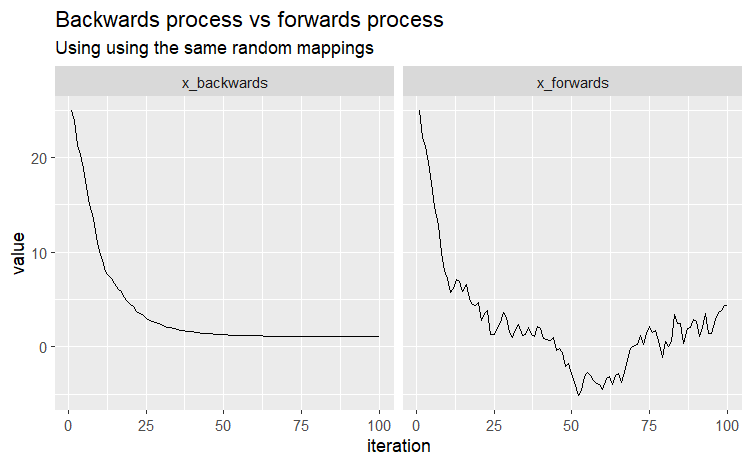
\includegraphics[width=0.7\linewidth]{images/backwardsvsforwards}
		\caption{The backwards, $\{\tilde{X}_n\}_{n\geq 1}$, and forwards, $\{X_n\}_{n\geq 1}$, process of the autoregressive normal system where $X_n,\tilde{X}_n$ are simulated using the same random mappings, $X_n=0.9X_{n-1}+Z_n, Z_n\sim N(0.1)$ and $X_0=25$.}
		\label{fig:backwardsvsforwards}
	\end{figure}
	
	Despite the difference in behaviour of the two processes, the marginal distributions of the forward and backward processes are the same, $X_n \overset{d}{=}\tilde{X}_n$. In fact, the following theorem shows that the expected distance over the joint distribution of $J(\tilde{X}_n,\tilde{X}_{n+1})$ realizes the same expected distance as the $J(X_n,Y_n)$ when CRN is used. 
	
	\begin{theorem}\label{thm:backwards}
		Let $X_n,Y_n$ be two copies of a Markov chain such that $X_n=f(\theta_n, X_{n-1})$ and $Y_n=f(\theta'_n, Y_{n-1})$. Suppose that $X_0=x$ and $Y_0=f(\theta,x)$ where $\theta\indep \theta_i$ for $i\in\{1\ldots, n\}$, then the expected distance between $X_n$ and $Y_n$ using CRN ($\theta_i=\theta'_i$) is equal to the expected distance between consecutive iterations of the backwards process, $\bar{X}_n$ and $\bar{X}_{n+1}$.
		$$E[d(X_n,Y_{n})\mid X_0=x]=E[d(\tilde{X}_n,\tilde{X}_{n+1})\mid \tilde{X}_0 = x]$$ 
		\begin{proof}
			\begin{align*}
				&E[d(X_n,Y_{n})\mid X_0=x] \\
				&=E[d[f(\theta_n,f(\theta_{n-1},\ldots f(\theta_1,x)\ldots)),f(\theta_n,f(\theta_{n-1},\ldots f(\theta_1,f(\theta,x))\ldots))]\mid X_0=x]\\
				&=E[d[f(\theta_n,f(\theta_{n-1},\ldots f(\theta_1,x)\ldots)),f(\theta_n,f(\theta_{n-1},\ldots f(\theta_1,f(\theta_{n+1},x))\ldots))]\mid X_0=x]\\
				&=E[d[f(\theta_1,f(\theta_{2},\ldots f(\theta_n,x)\ldots)),f(\theta_1,f(\theta_{2},\ldots f(\theta_n,f(\theta_{n+1},x))\ldots))]\mid \tilde{X}_0=x]\\
				&= E[d(\tilde{X}_n,\tilde{X}_{n+1})\mid \tilde{X}_0 = x]
			\end{align*}
		\end{proof}
	\end{theorem}
	
	This means that for initial values defined as in Theorem \ref{thm:backwards}, when CRN is an optimal coupling at iteration $n$, the expected distance between consecutive iterations of the backwards process is also the optimal coupling. 

	\subsection{Connection between CRN and the contraction condition}\label{subsec:contractioncond}
	Calculating contraction conditions are a common way to generate theoretical upper bounds on the Wasserstein distance between two copies of a Markov chain. The following is an example contraction condition. A survey of contraction conditions can be found in \cite{avcont}.
	
	\begin{definition}[Average contractive]
		A Markov chain is average contractive if for all $x,y$ $\pi-$everywhere,
		$$\gamma_{cont}=\sup_{x \not= x'} \frac{E[k(f(\theta, x),f(\theta, x'))]}{k(x,x')}<1$$
	\end{definition}
	
	Notice how the contraction rate implicitly uses CRN. That is, we apply the same $\theta$ in $f(\theta,x)$ and $f(\theta,x')$ to calculate the contraction rate.
	
	Implicitly using CRN to generate contraction conditions is not limited to average contraction rates. Anywhere where backwards processes are used to generate contraction rates, the CRN is implicitly assumed, by Theorem \ref{thm:backwards}. Local contractivity (see Definition 5 of \cite{localcont}) uses backwards processes and so by extension CRN. Theorem 5.1 of \cite{iteratedranfunc}, which provides sufficient conditions for geometric convergence uses backwards processes in the proof and again by extension CRN. Backwards processes are used more often in proofs, because they facilitate convergence to stationarity.
	
	\section{Appendix}
	\addtocontents{toc}{\protect\setcounter{tocdepth}{0}}
	\subsection{Proof of Proposition \ref{thm:equivinv4}}\label{sec:skorohod}
	
		\begin{proof}{Proof of Proposition \ref{thm:equivinv4}}\label{pf:skorohod}
		
		$\impliedby$: $|F^{-1}_{n}(U)-F^{-1}(U)| \to 0 \text{ w.p. 1}$ means that $F^{-1}_{n}(U) \to F^{-1}(U)$ almost surely, which means that $\mathcal{L}(F^{-1}_{n}(U)) \to \mathcal{L}(F^{-1}(U))$ in distribution. Since $F^{-1}_{n}(U)\sim \mathcal{L}(X_n)$ and $F^{-1}(U)\sim\mathcal{L}(X_{\infty})$, this implies 
		$\mathcal{L}(X_n)\to \mathcal{L}(X_{\infty})$.
		
		$\implies$
		This proof greatly resembles the proof of Theorem 10.1.1 (4) of \cite{firstlook}.
		
		Denote $D_{F^{-1}}\in [0,1]$ as the set of discontinuous points on $F^{-1}$ and $C_{F^{-1}}\in [0,1]$ as the set of continuous points on $F^{-1}$.
		
		Let $0<u<1$,  $\epsilon>0$, and choose $\omega$ such that $F^{-1}(u)-\epsilon<\omega<F^{-1}(u)$ and $\pi(\omega)=0$. Then $F(\omega)<u$ and since $F_{n}(\omega)\to F(\omega)$, for sufficiently large $n$, $F_{n}(\omega)<u$ and so, $F^{-1}(u)-\epsilon<\omega<F^{-1}_{n}(u)$. Thus,
		\begin{equation}\label{eq:skorohodinf}
			\lim \inf F_{n}^{-1}(u)\geq F^{-1}(u)
		\end{equation}
		
		Let $0<u<u'<1$ and choose $\omega$ such that $F^{-1}(u')<\omega<F^{-1}(u')+\epsilon$ and $\pi(\omega)=0$. Then $u<u'\leq F(F^{-1}(u'))\leq F(\omega)$ and since $F_{n}(\omega)\to F(\omega)$, for sufficiently large $n$, $u\leq F_{n}(\omega)$ and $F^{-1}_{n}(u)\leq \omega < F^{-1}(u')+\epsilon$. Thus,
		\begin{equation}\label{eq:skorohodsup}
			\lim \sup F_n^{-1}(u)\leq F^{-1}(u')
		\end{equation}
		
		By equation \ref{eq:skorohodinf} and equation \ref{eq:skorohodsup} if $F^{-1}$ is continuous at $u$ (ie. $u\in C_{F^{-1}}$), then $\lim_{n\to \infty} F^{-1}_{n}(u)= F^{-1}(u)$. Or in other words, $P(\lim_{n\to \infty} |F^{-1}_{n}(u)- F^{-1}(u)|=0\mid U\in C_{F^{-1}})=1$. %By the same reasoning, $\lim_{n\to \infty} F^{-1}_{y,n}(u)= F^{-1}(u)$, and so for $u\in C_{F^{-1}}$
%		\begin{equation}\label{eq:skorohodconvcont}
%			\lim_{n\to \infty} |F^{-1}_{x,n}(u)-F^{-1}_{y,n}(u)|\leq \lim_{n\to \infty} |F^{-1}_{x,n}(u)-F^{-1}(u)| + \lim_{n\to \infty} |F^{-1}(u)-F^{-1}_{y,n}(u)| =0
%		\end{equation}
		
		Next suppose that $U\sim Unif(0,1)$. Since $F^{-1}$ is non-decreasing on $(0,1)$, it has countably many discontinuous points and so $P(U\in D_{F^{-1}})=0$ (and $P(U\in C_{F^{-1}})=1$).
		
		Thus, the probability of $\lim_{n\to \infty} |F^{-1}_{n}(u)- F^{-1}(u)|=0$ is as follows,
		\begin{align*}
			&P(\lim_{n\to \infty} |F^{-1}_{n}(U)- F^{-1}(U)|=0)\\
			&\geq P( \lim_{n\to \infty} |F^{-1}_{n}(U)- F^{-1}(U)|=0\mid U\in C_{F^{-1}})P(U\in C_{F^{-1}}) \\
			&=1
		\end{align*}
		
%		then,
%		\begin{align*}
%			&P\left(\lim_{n\to \infty} |F^{-1}_n(U)-F^{-1'}_n(U)|=0\right) \\
%			&= P\left(\lim_{n\to \infty} |F^{-1}_n(U)-F^{-1'}_n(U)|=0\mid D_{F^{-1}}\right)P(D_{F^{-1}}) + P\left(\lim_{n\to \infty} |F^{-1}_n(U)-F^{-1'}_n(U)|=0\mid C_{F^{-1}}\right)P(C_{F^{-1}})\\
%			&=P\left(\lim_{n\to \infty} |F^{-1}_n(U)-F^{-1'}_n(U)|=0\mid D_{F^{-1}}\right)\times0 + 1\times 1\\
%			&=1
%		\end{align*}
		And so, when CRN is applied to the quantile function, $|F^{-1}_n(U)-F^{-1}(U)|\to 0$ w.p. 1.
	\end{proof}
	
%	The following is a theorem that we will use to prove that random variables simulated according to common random number converge almost surely. We've adjusted the theorem notation to describe distribution functions.
%	\begin{prop}[Theorem 2 of \cite{invconv}]\label{thm:invconvgen}
%		Let  $\{F_n\}_{n\geq 0}$ be a sequence of mappings. If
%		\begin{enumerate}
%			\item $\{F_n\}_{n\geq 0}$ is a sequence of injective mappings on a metric space
%			$(\mathbb{R}^d,k)$ and taking values in a locally compact metric space $([0,1],|\cdot|)$,
%			\item $F_n\to F$ uniformly on $\mathbb{R}^d$, 
%			\item $F^{-1}$ is a continuous mapping on $[0,1]$
%		\end{enumerate}
%		Then $F^{-1}_n\to F^{-1}$ uniformly on every compact set $K_0$ contained in $N_0=Interior[0,1]\cap_{n\geq 1}Im(F_n)$
%	\end{prop}
%	
%	Theorem \ref{thm:invconvgen} is a general theorem, but we are only interested in the theorem applied to distribution functions. Many of the requirements are already fulfilled for distribution functions (for example if $F_n\to F$ and $F$ is continuous then the convergence is uniform (see example 14.8 of \cite{billingsley}, theorem 1.1 of \href{https://researchers.ms.unimelb.edu.au/~xgge@unimelb/Files/Teaching/Advanced%20Probability%20(Semester%201%202020)/Lecture%20Notes.pdf}{this}), the metric space $([0,1],\lambda)$ is already locally compact, if $F^{-1}$ is continuous then $F$ is continuous \href{https://math.stackexchange.com/questions/541082/proving-the-inverse-of-a-continuous-function-is-also-continuous}{Why does Google always send me to mathStackExchange???} etc.), so we can rewrite theorem \ref{thm:invconvgen} as follows.
%	
%	\begin{prop}[Theorem 2 of \cite{invconv} adjusted for distribution functions]\label{thm:invconvgen}
%		Let  $\{F_n\}_{n\geq 0}$ be a sequence of mappings. If
%		\begin{enumerate}
%			\item $\{F_n\}_{n\geq 0}$ is a sequence of strictly increasing distribution functions on a metric space
%			$(\mathbb{R}^d,||^2)$ and taking values in $([0,1],||)$, 
%			\item $F_n\to F$ on $\mathbb{R}^d$
%			\item $F$ is a continuous, invertible mapping on $[0,1]$
%		\end{enumerate}
%		Then $F^{-1}_n\to F^{-1}$ uniformly on every compact set $K_0\in (0,1)$.
%	\end{prop}
%	 The following is the definition of uniform convergence, which will be used in the proof of Theorem \ref{thm:skorohod}.
%	 
%	\begin{definition}[Uniform convergence of functions]
%		The given the sequence of functions $F_{n}:(\mathbb{R}^d,||^2)\to ([0,1],||)$ and the target function $F:(\mathbb{R}^d,||^2)\to ([0,1],||)$,  $F_n\to F$ uniformly if for all $\epsilon >0$, there exists an $N\in\mathbb{N}$ such that for any $n\geq N$ and $x\in \mathbb{R}^d$, 
%		$$|F_n(x)-F(x)|\leq \epsilon$$
%	\end{definition}
%	
%%	This theorem implies the following result. Namely let $F$ be a target distribution function and 
%%	\begin{enumerate}
%%		\item $\{X_n(u)\}_{n\geq 1}$ be a sequence of random variables with $X_n(u)=F^{-1}_n(u)$, $F_n\to F$ on $\mathbb{R}^d$ and $F_n, n\geq 1$ is strictly increasing  on $\mathbb{R}^d$
%%		\item $\{X'_n(u)\}_{n\geq 1}$ be a sequence of random variables with $X'_n(u)=F^{'-1}_n(u)$, $F'_n\to F$ on $\mathbb{R}^d$ and $F_n, n\geq 1$ is  strictly increasing on $\mathbb{R}^d$
%%	\end{enumerate}
%%	
%%	Common random number simulation of $X_n, X'_n$, means that for each iteration $n$, we simulate $U_n\sim Unif(0,1)$ and generate the random variables, $X_n(U_n), X'_n(U_n)$, from the same $U_n$. 
%	
%\begin{proof}{Proof of Theorem \ref{thm:skorohod}}\label{pf:skorohod}
%	
%	%First note that conditions 1 and 2 of Proposition \ref{thm:invconvgen} are satisfied by the definitions of $X_n,X'_n$.
%	
%	Let $C_m=[\frac{1}{m}, 1-\frac{1}{m}]$, $m>2$ be a compact set. Then by definition of uniform convergence for any $\epsilon >0$, there exists an $N\in\mathbb{N}$ such that for any $n\geq N$  and $u\in C_m$, $|F^{-1}_{n}(u)-F^{-1}(u)|\leq \epsilon$
%
%	This means that 
%	$$P(\lim_{n\to\infty} |F^{-1}_n(u)-F^{-1}(u)|\leq \epsilon)\geq P(U\in C_m)=1-\frac{2}{m}$$
%	Since $m>2$ is arbitrary, we set $m\to\infty$ and so,
%	$$P\left(\lim_{n\to\infty} |F^{-1}_n(u)-F^{-1}(u)|\leq \epsilon\right)=1$$
%\end{proof}
	\newpage
	\subsection{Proof of Proposition \ref{prop:incr1}} \label{pf:incr1}
	\begin{proof}[Proof of Proposition \ref{prop:incr1}]
	Denote $g(\theta)=f(\theta,x)$ and $h(\theta)=f(\theta,y)$ for fixed $x$ and $y$.

	Since $g$ and $h$ are monotone in $\theta$ by assumption, if $\theta_1\leq \theta_1'$ and $\theta_2\leq \theta_2'$, then $g(\theta_1)\leq g(\theta_1')$ and $h(\theta_2)\leq h(\theta_2')$. By the quasi-antitone property of $k^p$,
	$$k\left(g(\theta_1),h(\theta_2)\right)^p+k\left(g(\theta_1'),h(\theta_2')\right)^p-k\left(g(\theta_1'),h(\theta_2)\right)^p-k\left(g(\theta_1),h(\theta_2')\right)^p\leq 0$$
	
	And so, $k(g(\theta_1),h(\theta_2))^p$ is quasi-antitone with respect to $\theta_1$ and $\theta_2$.
	
	Further, since $g$ and $h$ are right-continuous functions, $k(g(\theta_1),h(\theta_2))^p$ is right-continuous with respect to $\theta_1,\theta_2$ and so $k(g(\theta_1),h(\theta_2))^p$ is QAC with respect to $\theta_1,\theta_2$. We can then apply Proposition \ref{prop:interval}. 
	\begin{align*}
		W_p(\mathcal{L}(X), \mathcal{L}(Y)) &=\left(\inf_{\mathcal{J}(X,Y)}E[k(X,Y)^p]\right)^{1/p}\\
		&=\left(\inf_{\mathcal{J}(\theta_1,\theta_2)}E[k(g(\theta_1),h(\theta_2))^p] \right)^{1/p}\\
		%&=\inf_{\mathcal{J}(U,V)}E[k(g(F^{-1}_{\theta}(U)),h(F^{-1}_{\theta}(V)))] \\
		&=\left(E[k(g(F^{-1}_{\theta}(U)),h(F^{-1}_{\theta}(U)))^p]\right)^{1/p} &\text{by Prop \ref{prop:interval}}\\
		&=\left(E[k(g(\theta),h(\theta))^p]\right)^{1/p}\\
		&=\left(E[k(f(\theta,x),f(\theta,y))^p]\right)^{1/p}
	\end{align*}
	
	The second equality is true because $X=g(\theta)$ and $Y=h(\theta)$ by definition and so every coupling $J(\theta_1,\theta_2)$ maps to a coupling in $J(X,Y)$. 
\end{proof}
%	\begin{proof}[Proof of Proposition \ref{prop:incr1}]
%		Let $F$ be the distribution function of $\theta$ such that $\theta=F^{-1}(U)$ and $\theta'=F^{-1}(V)$ where $U,V\sim Unif(0,1)$.
%
% Since $f(\cdot, x)$ and $f(\cdot, y)$ are non-decreasing functions, if $\theta_1\leq\theta_1'$ and $\theta_2\leq\theta_2'$, then $f(\theta_1,x)\leq f(\theta_1',x)$ and $f(\theta_2,y)\leq f(\theta_2',y)$. By the quasi-antitone property of $k$,
%		$$k\left(f(\theta_1,x),f(\theta_2,y)\right)+k\left(f(\theta_1',x),f(\theta_2',y)\right)-k\left(f(\theta'_1,x),f(\theta_2,y)\right)-k\left(f(\theta_1,x),f(\theta'_2,y)\right)\leq 0$$
%		
%		And so, $k(f(\theta_1, x), f(\theta_2, y))$ is quasi-antitone with respect to $\theta_1$ and $\theta_2$.
%		
%		Further, since $f(\cdot, x)$ and $f(\cdot, y)$ are right-continuous functions, $k(f(\theta_1, x), f(\theta_2, y))$ is right-continuous with respect to $\theta_1,\theta_2$ and so $k(f(\theta_1, x), f(\theta_2, y))$ is QAC with respect to $\theta_1,\theta_2$. We can then apply Proposition \ref{prop:interval}. 
%		\begin{align*}
%			W_p(\mathcal{L}(X), \mathcal{L}(Y)) &=\inf_{\mathcal{J}(X,Y)}E[k(X,Y)]\\
%			&=\inf_{\mathcal{J}(U,V)}E[k(f(F^{-1}_{\theta}(U),x),f(F^{-1}_{\theta}(V),y))] \\
%			&=E[k(f(F^{-1}_{\theta}(U),x), f(F^{-1}_{\theta}(U),y))] &\text{by Prop \ref{prop:interval}}\\
%			&=E[k(f(\theta,x), f(\theta,y))] &\text{Since $\mathcal{L}(F^{-1}_{\theta}(U))=\mathcal{L}(\theta)$}
%		\end{align*}
%	\end{proof}
%	\newpage
%	\subsection{Proof of Theorem \ref{thm:iff}} 
%	To prove Theorem \ref{thm:iff} we introduce Lemma \ref{lem:crngen} and Lemma \ref{lem:crnnotgen}. Together they provide the necessary and sufficient conditions required in Theorem \ref{thm:iff}.
%	Denote  $A =(I_x\cap I_y)\cup (D_x\cap D_y)$.
%	
%		\begin{lemma}[Sufficient conditions for when CRN is maximal coupling]\label{lem:crngen}
%		\begin{equation}\label{eqn:probA1}
%			P(\theta \in A)=1\implies W_{||\cdot||^2}(\mathcal{L}(X),\mathcal{L}(Y)) %=\inf_{J(\theta_U,\theta_V)} E[(f(\theta_U, x)-f(\theta_V, y))^2] 
%			= E[(f(\theta, x)-f(\theta, y))^2]
%		\end{equation}
%		
%		The proof is in subsection \ref{pf:crngen}.
%	\end{lemma}
%	
%	\begin{lemma}[Sufficient conditions for when CRN is not the maximal coupling]\label{lem:crnnotgen}
%		\begin{equation}\label{eqn:probA2}
%		P(\theta \in A)<1\implies 	W_{||\cdot||^2}(\mathcal{L}(X),\mathcal{L}(Y)) 
%			< E[(f(\theta, x)-f(\theta, y))^2]
%		\end{equation}
%		
%		The proof is in subsection \ref{sec:crnnotgen}.
%	\end{lemma}
%
%%Suppose that $I_z,D_z,I_z^C, D_z^C$ can all be written as a countable union of disjoint intervals for $z\in\{x,y\}$. That is, 
%%\begin{align*}
%%	I_z=\dot{\bigcup}_{n=1}^{\infty}I_{z,n} & & D_z=\dot{\bigcup}_{n=1}^{\infty}D_{z,m} & & 
%%	 I_z^C=\dot{\bigcup}_{n=1}^{\infty}I_{z,n}^C & & D^C_z=\dot{\bigcup}_{n=1}^{\infty}D^C_{z,n}
%%\end{align*}
%%
%%\begin{lemma}
%%	The set $A =(I_x\cap I_y)\cup (D_x\cap D_y)$ ce be written as the union of countable disjoint intervals.
%%	
%%	\begin{proof}
%%		\begin{align*}
%%		A &=(I_x\cap I_y)\cup (D_x\cap D_y)\\
%%		&=(\dot{\bigcup}_{n=1}^{\infty} \dot{\bigcup}_{m=1}^{\infty} I_{x,n}\cap I_{y,m})\cup (\dot{\bigcup}_{n=1}^{\infty} \dot{\bigcup}_{m=1}^{\infty} D_{x,n}\cap D_{y,m})
%%		\end{align*}
%%	\end{proof}
%%\end{lemma}
%	
%	\subsubsection{Proof of Lemma \ref{lem:crngen}}
%%	To prove the Lemma \ref{lem:crngen} we define the following specific notation.
%%	For fixed $x, y \in \mathbb{R}$, let $X = f(\theta_U,x)$ and $Y = f(\theta_V,y)$ be random functions with measurable $f: \mathbb{R}^2 \mapsto \mathbb{R}$ and $\theta_U = F^{-1}_{\theta}(U)$ and $\theta_V = F^{-1}_{\theta}(V)$ with $U,V\sim Unif(0,1)$. Let $I_z, D_z$ be defined as in Section \ref{sec:background}.
%%	Define the set $A =(I_x\cap I_y)\cup (D_x\cap D_y)$ which is where either $f(\cdot, x)$ and $f(\cdot, y)$ are increasing over the same intervals of $\theta$ or decreasing over the same intervals of $\theta$.
%%	
%%	Note that 
%%	\begin{align}\label{eqn:infdist}
%%		W_2(\mathcal{L}(X),\mathcal{L}(Y)) =\inf_{\mathcal{J}(X,Y)}E[(X-Y)^2]
%%		=E[X^2]+E[Y^2]- 2 \sup_{\mathcal{J}(X,Y)}E[XY]
%%	\end{align}
%%	Since $E[X^2]$ and $E[Y^2]$ must remain constant, finding $\sup_{\mathcal{J}(X,Y)}E[XY]$ is equivalent to finding $\inf_{\mathcal{J}(X,Y)}E[(X-Y)^2]$. 
%	\begin{proof}\label{pf:crngen}
%		Assume $P(A)=1$.
%		Fix $x,y$ and denote $g(U) = f(F^{-1}_{\theta}(U), x) $ and  $h(V) = f(F^{-1}_{\theta}(V), y)$. We write $\mathcal{J}(U,V)$ to be the set of joint distributions such that $\mathcal{L}(U), \mathcal{L}(V)= Unif(0,1)$. 
%		
%%		First we show that
%%		\begin{equation}\label{eqn:equal}
%%			\sup_{\mathcal{J}(\theta_U, \theta_V)} E[g(U),h(V)1_{A}]= E[g(U)h(U)1_{A}]
%%		\end{equation}
%%		Let $P=\{x_1,x_2,\ldots, x_{p}\}$ be the local extrema. I can partition the set $A$ by $P$, which will generate a set of finite disjoint union of intervals $B_1,B_2,
%%		\ldots B_{p+1}$ such that 
%%		\begin{itemize}
%%			\item $B_1=(-\infty,x_1)\cap (I_x\cap I_y)$, $B_{p+1}=(x_p,\infty)\cap (I_x\cap I_y)$ and for $i\in (2,\ldots, p)$, $B_i=(x_{i-1},x_{i})\cap (I_x\cap I_y)$
%%			\item $\dot{\bigcup}_{i=1}^{p+1} B_i= (I_x\cap I_y)$  ($B_i$ may be empty)
%%			\item For each $B_i\neq \emptyset$, if $\theta_1, \theta_2\in B_i$ and $\theta_1<\theta_2$, then $f(\theta_1,x)\leq f(\theta_2,x)$ and $f(\theta_1,y)\leq f(\theta_2,y)$.
%%		\end{itemize}
%		
%%		By Lemma \ref{lem:countable}, $I_x,I_y$ can be written as a sequence of countable disjoint intervals $I_x=\dot{\bigcup}_{n\geq 1}B_n{x,n}$ and $I_y=\dot{\bigcup}_{n\geq 1}B_{y,n}$. The intersection $I_x\bigcap I_y$ can then be written as a countable union of disjoint intervals $I_x\bigcap I_y=\dot{\bigcup}_{n\geq 1}\dot{\bigcup}_{m\geq 1}B_{x,n}\bigcap B_{y,m}$. Denote $\{B_n\}_{n\geq 1}$ to be a countable union of disjoint intervals such that $I_x\bigcap I_y = \dot{\bigcup}_{n\geq 1} B_n$. Note that for each for each $B_n$, if $\theta_1, \theta_2\in B_n$ and $\theta_1<\theta_2$, then $f(\theta_1,x)\leq f(\theta_2,x)$ and $f(\theta_1,y)\leq f(\theta_2,y)$.
%%		
%%		By similar reasoning, we can write $D_x\bigcap D_y=\dot{\bigcup}_{n\geq 1} B'_n$ where $B'_n$ are disjoint intervals. Note that for each $B'_n$, if $\theta_1, \theta_2\in B'_n$ and $\theta_1<\theta_2$, then $f(\theta_1,x)\geq f(\theta_2,x)$ and $f(\theta_1,y)\geq f(\theta_2,y)$
%		
%		By assumption $I_x=I_y$ and $D_x=D_y$ can be written as the union of countable disjoint intervals. So we write $I_x=\dot{\bigcup}_{n= 1}^{\infty}B_n$ and  $D_x=\dot{\bigcup}_{n= 1}^{\infty}B'_n$ where $B_n, B'_n$ are intervals.
%		
%%		Next define the set of finite disjoint union of intervals $B'_1,B'_2,
%%		\ldots B'_{p+1}$ such that 
%%		\begin{itemize}
%%			\item $B'_1=(-\infty,x_1)\cap A \setminus (I_x\cap I_y)$, $B'_{p+1}=(x_p,\infty)\cap A \setminus (I_x\cap I_y)$ and for $i\in (2,\ldots, p)$, $B'_i=(x_{i-1},x_{i})\cap A \setminus (I_x\cap I_y)$
%%			\item $\dot{\bigcup}_{i=1}^{p+1} B'_i= A \setminus (I_x\cap I_y)$  ($B'_i$ may be empty)
%%			\item For each $B'_i\neq \emptyset$, if $\theta_1, \theta_2\in B'_i$ and $\theta_1<\theta_2$, then $f(\theta_1,x)\geq f(\theta_2,x)$ and $f(\theta_1,y)\geq f(\theta_2,y)$.
%%		\end{itemize}
%		
%		%Denote $ \{B_{n}\}_{n\geq 1}$ to be a countable partition of $I_x\bigcap I_y=\bigcup_{n=1}^{\infty}{B_{n}}$ and $\{B'_{n}\}_{n\geq 1}$ to be a countable partition of $A/(I_x\bigcap I_y)=\bigcup_{n=1}^{\infty}{B'_{n}}$. Such a set exists, because the interior of $I_z,D_z$, $I_z^o,D_z^o$, is an open set, which can be written as a union of countable disjoint open intervals. The remainder $I_z/I_z^o, D_z/D_z^o$ belong to the boundary of $I_z,D_z$. The union of the boundary of $I_z,D_z$ and the countable disjoint open intervals generates a union of countable disjoint intervals.
%		
%		We can then show that the supremum of $ E[(g(U)-h(V))^2]$ is bounded above by $E[(g(U)-h(U))^2]$ as follows,
%		\begin{align*}
%			(\star)&=\inf_{\mathcal{J}(X,Y)} E[(X-Y)^2] \\
%			&=\inf_{\mathcal{J}(U,V)} E[(g(U)-h(V))^2] \\
%			&=\inf_{\mathcal{J}(U,V)} E[(g(U)-h(V))^2\left(I_{U\in I_x}I_{V\in I_x} + I_{U\in D_x}I_{V\in D_x} + I_{U\in I_x}I_{V\in D_x} + I_{U\in D_x}I_{V\in I_x}\right)]\\
%			&\geq\inf_{\mathcal{J}(U,V)} E[(g(U)-h(V))^2\left(I_{U\in I_x}I_{V\in I_x} + I_{U\in D_x}I_{V\in D_x}\right)]\\
%			&\geq\inf_{\mathcal{J}(U,V)} E\left[(g(U)-h(V))^2\left(\sum_{n=1}^{\infty}I_{U\in B_n}I_{V\in B_n} + \sum_{n=1}^{\infty}I_{U\in B'_n}I_{V\in B'_n}\right)\right]\\
%			%&\geq \inf_{\mathcal{J}(U,V)} E[(g(U)-h(V))^2I_{U\in I_x}I_{V\in I_x}] + \inf_{\mathcal{J}(U,V)} E[(g(U)-h(V))^2I_{U\in D_x}I_{V\in D_x}]\\
%			%&= \inf_{\mathcal{J}(U,V)} E[(g(U)-h(V))^2I_{U\in I_x}I_{V\in I_x}] + \inf_{\mathcal{J}(U,V)} E[((-g(U))-(-h(V)))^2I_{U\in D_x}I_{V\in D_x}]\\
%			&\geq \sum_{n=1}^{\infty}\inf_{\mathcal{J}(U,V)} E[(g(U)-h(V))^2I_{U\in B_n}I_{V\in B_n}] + \sum_{n=1}^{\infty} \inf_{\mathcal{J}(U,V)} E[(g(U)-h(V))^2I_{U\in B'_n}I_{V\in B'_n}]\\
%			&= \sum_{n=1}^{\infty}\inf_{\mathcal{J}(U,V)} E[(g(U)-h(V))^2I_{U\in B_n}I_{V\in B_n}] + \sum_{n=1}^{\infty} \inf_{\mathcal{J}(U,V)} E[((-g(U))-(-h(V)))^2I_{U\in B'_n}I_{V\in B'_n}]\\
%			&= \sum_{n=1}^{\infty} E[(g(U)-h(U))^2I_{U\in B_n}] + \sum_{n=1}^{\infty} E[((-g(U))-(-h(U)))^2I_{U\in B'_n}]\\
%			&=E[(g(U)-h(U))^2]
%		\end{align*}
%%		\begin{align*}
%%			(\star)&=\sup_{\mathcal{J}(X,Y)} E[XY] \\
%%			&=\sup_{\mathcal{J}(U,V)} E[g(U)h(V)] \\
%%			&=\sup_{\mathcal{J}(U,V)} E[g(U)h(V)1_{A}] &\text{Since $P(A)=1$}\\
%%			&\leq \sup_{\mathcal{J}(U,V)} E[g(U)h(V)1_{I_x\cap I_y}] + \sup_{\mathcal{J}(U,V)} E[g(U)h(V)1_{A \setminus (I_x\cap I_y) }] &\text{this is not correct}\\
%%			&= \sup_{\mathcal{J}(U,V)} E[g(U)h(V)1_{I_x\cap I_y}] + \sup_{\mathcal{J}(U,V)} E[(-g(U))(-h(V))1_{A \setminus (I_x\cap I_y) }] \\
%%			%&= \sup_{\mathcal{J}(U,V)} E\left[\sum_{i=1}^{p+1}g(U)h(V)1_{B_{i}}\right] + \sup_{\mathcal{J}(U,V)} E\left[\sum_{i = 1}^{p+1}(-g(U))(-h(V))1_{B'_i}\right] \\
%%			&= \sup_{\mathcal{J}(U,V)} \sum_{i=1}^{\infty}E\left[g(U)h(V)1_{B_i}\right] + \sup_{\mathcal{J}(U,V)} \sum_{i=1}^{\infty}E\left[(-g(U))(-h(V))1_{B'_i}\right] \\%&\text{By DCT (thm 1.5.8 of \cite{durrett})}\\
%%			&\leq \sum_{i=1}^{\infty}\sup_{\mathcal{J}(U,V)}E[g(U)h(V)1_{B_i}] + \sum_{i=1}^{\infty}\sup_{\mathcal{J}(U,V)}E[(-g(U))(-h(V))1_{B'_i}]\\
%%			&= \sum_{i=1}^{\infty}E[g(U)h(U)1_{B_i}] + \sum_{i= 1}^{\infty}E[(-g(U))(-h(U))1_{B'_i}] &\text{By Proposition 2.2 of \cite{crn}}\\
%%			&= E[g(U)h(U)1_{I_x\cap I_y}] + E[(-g(U))(-h(U))1_{A \setminus (I_x\cap I_y) }]\\
%%			&= E[g(U)h(U)1_{A}]\\
%%			&= E[g(U)h(U)] &\text{Since $P(A)=1$}
%%		\end{align*}
%%		
%%		Since $E[g(U)h(U)] \leq \sup_{\mathcal{J}(U,V)} E[g(U)h(V)] \leq E[g(U)h(U)]$, equality follows. %Note that Proposition \ref{prop2} can still be applied even if $g(U)h(U)1_{J_k}$ and $g(U)h(U)1_{L_k}$ are no longer the product of right continuous functions, which is a result of the fact that $1_{J_k}$ may not necessarily be right continuous. This is because the theorem still applies by discussions in Section 4 of \cite{cambanis1976} that note that rather than requiring that $f(\theta,x)$ be right continuous it is simply necessary to assume that the discontinuous points are countable and have left and right limits. 
%%		
%%%		If $P(A)=1$.
%%%		\begin{align*}
%%%			\sup_{\mathcal{J}(U,V)} E[g(U)h(V)]
%%%			= \sup_{\mathcal{J}(U,V)} E[g(U)h(V)1_{A}]= E[g(U)h(U)1_{A}] = E[g(U)h(U)]
%%%		\end{align*}
%%		
%%%		By similar reasoning to the proof of Proposition \ref{prop:incr1}, $\sup_{\mathcal{J}(U,V)} E[g(U)h(V)]=\sup_{\mathcal{J}(X,Y)} E[XY]$
%%%		By equation \ref{eqn:infdist}, equation \ref{eqn:probA1} follows,
%%%		$$W_{||\cdot||^2}(\mathcal{L}(X),\mathcal{L}(Y))=\inf_{\mathcal{J}(X,Y)}E[(X-Y)^2]=E[(f(F_{\theta}^{-1}(U), x)-f(F_{\theta}^{-1}(U), y))^2]$$
%%		
%%		Finally using the above equation, $(\star)$, we show that the Wasserstein distance is equal to the expected distance when common random number is applied,
%%		\begin{align*}
%%			W_2(\mathcal{L}(X),\mathcal{L}(Y)) &=\inf_{\mathcal{J}(X,Y)}E[(X-Y)^2] \\
%%			& =E[X^2]+E[Y^2]- 2 \sup_{\mathcal{J}(X,Y)}E[XY] \\
%%			& =E[X^2]+E[Y^2]- 2E[g(U)h(U)] &\text{by Equation $(\star)$} \\
%%			& =E[X^2]+E[Y^2]- 2E[f(F^{-1}_{\theta}(U), x)f(F^{-1}_{\theta}(U), y)] \\
%%			& =E[f(\theta, x)^2]+E[f(\theta, y)^2]- 2E[f(\theta, x)f(\theta, y)] \\
%%			& =E[(f(\theta, x)-f(\theta, y))^2]
%%		\end{align*}
%	\end{proof}
%\newpage
%\subsection{Theorem \ref{thm:ab}}\label{sec:ab}
%
%We denote $I_g, D_g\in [0,1]$ where $I_g$ and $D_g$ represent the regions of $u$ where $g(u)$ is non-decreasing and non-increasing, respectively.
%\begin{align}\label{eq:igdg}
%	I_g&=\{u\in [0,1] \mid  \exists \epsilon>0 \text{ s.t. }\forall u_1,u_2\in B_{\epsilon}(u) \text{, if }u_1<u_2 \text{ then }g(u_1)\leq g(u_2)\}\\
%	D_g&=\{u\in [0,1] \mid  \exists \epsilon>0 \text{ s.t. }\forall u_1, u_2\in B_{\epsilon}(u) \text{, if }u_1<u_2 \text{ then }g(u_1)> g(u_2)\}
%\end{align}
%
%Next we present joint random variables, $U,V^*$, that generates a lower expected distance than CRN when the regions of $I_g\cap D_h$ and  $D_g\cap I_h$ have positive probability. 
%
%\begin{theorem}\label{thm:ab}
%	Let $X=g(U)$ and $Y=h(V)$ be defined on the Polish metric space $(\mathbb{R},k)$ where $k$ is QAC, $\mathcal{L}(X),\mathcal{L}(Y) \in P_p(\mathbb{R})$, and $U,V\sim \unif(0,1)$.
%	
%	If there is an interval $(a,b)$ such that $P(U\in (a,b))>0$ and either $(a,b)\in I_g\cap D_h$ or $(a,b)\in D_g\cap I_h$ then 
%	$$E[k(g(U),h(V^*))]\leq E[k(g(U),h(U))]$$
%	
%	Where
%	\begin{equation}\label{eq:Vstar}
%		V^*=
%		\begin{cases}
%			U & \text{if } U\notin (a,b)\\
%			%F_{X_{B_i}}^{-1}(1-F_{X_{B_i}}(U)) & \text{if } U\in F_{\theta}(B_i)=(a_i,b_i)
%			a+b-U & \text{if } U\in (a,b)
%		\end{cases}
%	\end{equation}
%\end{theorem}
%
%We use the above construction of $(U,V^*)$ to show that CRN is not the optimal coupling for a two-step random logistic map (despite being the optimal coupling for a one-step random logistic map). See Example \ref{ex:randomlogmap} for more details. 
%
%		We introduce the notation and Lemmas \ref{lem:WVinUU} before providing a proof of Lemma \ref{lem:crnnotgen}.
%		\begin{itemize}
%			\item $g(W)=f(F^{-1}_{\theta}(W),x)$ and $h(V)=f(F^{-1}_{\theta}(V),y)$ where $x,y$ are fixed, $F_{\theta}$ is the distribution function on $\theta$, and $V,W\sim \unif(0,1)$.
%		\end{itemize}
%		
%		By assumption $A^C$ can be written as the union of countably many disjoint intervals, $A^C=\dot{\bigcup}_{i= 1}^{\infty}B_i$. %By definition of $A^C$, for each $B_i$ such that $P(B_i)>0$, if $\theta_1, \theta_2\in B_i$ and $\theta_1<\theta_2$, then either $f(\theta_1,x)>f(\theta_2,x)$ and $f(\theta_1,y)<f(\theta_2,y)$ or $f(\theta_1,x)<f(\theta_2,x)$ and $f(\theta_1,y)>f(\theta_2,y)$.
%		
%%		\begin{lemma}
%%		The complement of $A$ is $A^C=(I_x^C\cap D_y^C)\cup(D_x^C\cap I_y^C)$ and $A^C$ can be written as the finite disjoint union of intervals, where $I_x^C\cap D_y^C=\dot{\bigcup}_{i=1}^{n}B_i$ and $I_y^C\cap D_x^C=\dot{\bigcup}_{i=1}^{m}C_i$. Further if $\theta_1, \theta_2\in B$ and $\theta_1<\theta_2$, then $f(\theta_1,x)>f(\theta_2,x)$ and $f(\theta_1,y)<f(\theta_2,y)$. Further if $\theta_1, \theta_2\in C$ and $\theta_1<\theta_2$, then $f(\theta_1,x)<f(\theta_2,x)$ and $f(\theta_1,y)>f(\theta_2,y)$.
%%		
%%		\begin{proof}
%%			\begin{align*}
%%				A^C&= \left((I_x\cap I_y)\cup (D_x\cap D_y)\right)^C\\
%%				&=(I_x^C\cup I_y^C)\cap (D_x^C\cup D_y^C)\\
%%				&=(I_x^C\cap D_x^C)\cup (I_x^C\cap D_y^C)\cup(I_y^C\cap D_x^C)\cup (I_y^C\cap D_y^C)\\
%%				&=(I_x^C\cap D_y^C)\cup(I_y^C\cap D_x^C)
%%			\end{align*}
%%			
%%	 Let $P=\{x_1,x_2,\ldots, x_{p}\}$ be the turning points. I can partition the set $I_x^C\cap D_y^C$ by $P$, which will generate a set of finite disjoint union of intervals $B_1,B_2,
%%	 \ldots B_{p+1}$ such that 
%%	 \begin{itemize}
%%	 	\item $B_1=(-\infty,x_1)\cap A^C$, $B_{p+1}=(x_p,\infty)\cap A^C$ and for $i\in (1,2,\ldots, p)$, $B_i=(x_{i},x_{i+1})\cap A^C$
%%	 	\item $\dot{\bigcup}_{i=1}^{p+1} B_i=A^C$  ($B_i$ may be empty)
%%	 	\item For each $B_i$ such that $P(B_i)>0$, if $\theta_1, \theta_2\in B_i$ and $\theta_1<\theta_2$, then either $f(\theta_1,x)>f(\theta_2,x)$ and $f(\theta_1,y)<f(\theta_2,y)$ or $f(\theta_1,x)<f(\theta_2,x)$ and $f(\theta_1,y)>f(\theta_2,y)$.
%%	 \end{itemize}
%%	 Finally, note that the turning points themselves do not belong to $A^C$ (ie. $P\notin A^C$). In fact, $P\in I_x,I_y, D_x$, and $D_y$.
%%		\end{proof}
%%		\end{lemma}
%	
%	Next denote the interval $F_{\theta}(B_i)=(a_i,b_i)\subset [0,1]$ %we define the random variable $X_{B_{i}}\sim \unif(F_{\theta}(B_i))$ and the transformation $T_i:B_i\to [0,1]$ such that $T_i(x)=F_{X_{B_{i}}}(x)=\lambda((0,x)\cap F_{\theta}(B_i))/\lambda(F_{\theta}(B_i))$. Note that $T_i(X_{B_i})\sim \unif(0,1)$ (see Exercise 1.2.4 of \cite{durrett}).
%%	\begin{itemize}
%%		\item If $y<0$, $P(T(X_B)\leq y)=P(F_{X_B}(X_B)\leq y)=0$
%%		\item If $y>1$, $P(T(X_B)\leq y)=P(F_{X_B}(X_B)\leq y)=1$
%%		\item If $0\leq y \leq 1$, $P(T(X_B)\leq y)=P(F_{X_B}(X_B)\leq y)=P(X_B\leq F_{X_B}^{-1}(y))=F_{\theta}(F_{X_B}^{-1}(y))=y$
%%	\end{itemize}
%	and the following random variables $U,W,V$ as follows.
%	
%	Define $U\sim \unif(0,1)$, $W=U$ and 
%	\begin{equation}\label{eq:V}
%		V=
%		\begin{cases}
%			U & \text{if } U\in F_{\theta}(A)\\
%			F_{U_{B_i}}^{-1}(1-F_{U_{B_i}}(U)) & \text{if } U\in F_{\theta}(B_i) \text{ for each } i
%		\end{cases}
%	\end{equation}
%	
%	Where $U_{B_i}\sim \unif(F_{\theta}(B_i))$. First note that $B_i$ is an interval and so, by continuity of $F_{\theta}$, $F_{\theta}(B_i)=(a_i,b_i)$ is an interval. This means that the CDF of $U_{B_i}$ is $F_{U_{B_i}}(x)=\frac{x-a_i}{b_i-a_i}$, the inverse CDF is $F^{-1}_{U_{B_i}}(x)=(b_i-a_i)x+a_i$, and $F_{U_{B_i}}^{-1}(1-F_{U_{B_i}}(x))=a_i+b_i-x$. Thus equation \ref{eq:V} can be written as follows,
%	
%	\begin{equation}\label{eq:V1}
%		V=
%		\begin{cases}
%			U & \text{if } U\in F_{\theta}(A)\\
%			%F_{X_{B_i}}^{-1}(1-F_{X_{B_i}}(U)) & \text{if } U\in F_{\theta}(B_i)=(a_i,b_i)
%			a_i+b_i-U & \text{if } U\in F_{\theta}(B_i)=(a_i,b_i)
%		\end{cases}
%	\end{equation}
%	
%	Since $F_{\theta}$ is invertible, and $A, B_1, B_2,\ldots$ is a partition of $\mathbb{R}$, $\dot{\bigcup}_{i\geq 1} F_{\theta}(B_i)\dot{\cup} F_{\theta}(A)=[0,1]$, so $V$ is well defined. Finally note that for all $U\in F_{\theta}(A^C)/\{0.5\}$, $V\neq U$ and so $P(V=U)=0$ (this is because $F_{\theta}$ is invertible and thus atomless, so $P(U=0.5)=0$).
%	
%	
%	We've defined $W,V$ in terms of $U$, which defines their joint distribution, but we want to show that their marginal distributions are $\unif(0,1)$ so that $J(\L(W),\L(V))\in \mathcal{J}(\L(U),\L(U))$.
%	
%	\begin{lemma}\label{lem:WVinUU}
%		For $W,V$ defined above, $J(\L(W),\L(V))\in \mathcal{J}(\L(U),\L(U))$
%	\end{lemma}
%	\begin{proof}
%		It is clear that $W\sim \unif(0,1)$. We must only show that $V\sim \unif(0,1)$.
%		
%		Define $C\in \mathcal{B}(0,1)$.
%		\begin{align*}%\label{eq:Vunif1}
%			P(V\in C)&=P(V\in C\mid U\in F_{\theta}(A))P(U\in F_{\theta}(A))+\sum_{i=1}^{\infty} P(V\in C\mid U\in F_{\theta}(B_i))P(U\in F_{\theta}(B_i))\\
%			&=P(U\in C\mid U\in F_{\theta}(A))P(U\in F_{\theta}(A))+\sum_{i=1}^{\infty} P(a_i+b_i-U\in C\mid U\in (a_i,b_i))\lambda(F_{\theta}(B_i))\\
%			&=\lambda(C\cap F_{\theta}(A))+\sum_{i=1}^{\infty} P(a_i+b_i-U\in C\mid U\sim \unif(a_i,b_i))\lambda(F_{\theta}(B_i))\\
%			&=\lambda(C\cap F_{\theta}(A))+\sum_{i=1}^{\infty} P(U'\in C\mid U'\sim \unif(a_i,b_i))\lambda(F_{\theta}(B_i))\\
%			&=\lambda(C\cap F_{\theta}(A))+\sum_{i=1}^{\infty} \frac{\lambda(C\cap (a_i,b_i))}{\lambda(a_i,b_i)}\lambda(F_{\theta}(B_i))\\
%			&=\lambda(C\cap F_{\theta}(A))+\sum_{i=1}^{\infty} \frac{\lambda(C\cap F_{\theta}(B_i))}{\lambda(F_{\theta}(B_i))}\lambda(F_{\theta}(B_i))\\
%			&=\lambda(C\cap F_{\theta}(A))+\sum_{i=1}^{\infty} \lambda(C\cap F_{\theta}(B_i))\\
%			&=\lambda(C)
%		\end{align*}
%		
%%		\begin{align*}
%%			&=\lambda(U\in C\cap F_{\theta}(A))+\sum_{i=1}^{\infty} P(a_i+b_i-U\in C\mid U\in (a_i,b_i))\lambda(F_{\theta}(B_i))\\
%%			&= \lambda(U\in C\cap F_{\theta}(A)) + \sum_{i=1}^{\infty} P(F_{X_{B_i}}^{-1}(1-F_{X_{B_i}}(U))\in C\mid U\in F_{\theta}(B_i))P(U\in F_{\theta}(B_i))\\
%%			&= \lambda(C\cap F_{\theta}(A)) + \sum_{i=1}^{\infty} P(F_{X_{B_i}}^{-1}(1-F_{X_{B_i}}(X_{B_i}))\in C)\lambda(F_{\theta}(B_i))\\
%%			&= \lambda(C\cap F_{\theta}(A)) + \sum_{i=1}^{\infty} P(F_{X_{B_i}}^{-1}(U)\in C)\lambda(F_{\theta}(B_i))\\
%%			&= \lambda(C\cap F_{\theta}(A)) + \sum_{i=1}^{\infty} P(X_{B_i}\in C)\lambda(F_{\theta}(B_i))\\
%%			&= \lambda(C\cap F_{\theta}(A)) + \sum_{i=1}^{\infty} \frac{\lambda(C\cap B_i)}{\lambda(F_{\theta}(B_i))}\lambda(F_{\theta}(B_i))\\
%%			&=\lambda(C)\\
%%			&=P(U\in C)
%%		\end{align*}
%%		\begin{align*}%\label{eq:Vunif1}
%%			P(V\in C)&=P(V\in C\mid U\in F_{\theta}(A))P(U\in F_{\theta}(A))+\sum_{i=1}^{\infty} P(V\in C\mid U\in F_{\theta}(B_i))P(U\in F_{\theta}(B_i))\\
%%			&= \lambda(U\in C\cap A) + \sum_{i=1}^{\infty} P(F_{X_{B_i}}^{-1}(1-F_{X_{B_i}}(U))\in C\mid U\in F_{\theta}(B_i))P(U\in F_{\theta}(B_i))\\
%%			&= \lambda(C\cap A) + \sum_{i=1}^{\infty} P(F_{X_{B_i}}^{-1}(1-F_{X_{B_i}}(X_{B_i}))\in C)\lambda(F_{\theta}(B_i))\\
%%			&= \lambda(C\cap A) + \sum_{i=1}^{\infty} P(F_{X_{B_i}}^{-1}(U)\in C)\lambda(F_{\theta}(B_i))\\
%%			&= \lambda(C\cap A) + \sum_{i=1}^{\infty} P(X_{B_i}\in C)\lambda(F_{\theta}(B_i))\\
%%			&= \lambda(C\cap A) + \sum_{i=1}^{\infty} \frac{\lambda(C\cap B_i)}{\lambda(F_{\theta}(B_i))}\lambda(F_{\theta}(B_i))\\
%%			&=\lambda(C)\\
%%			&=P(U\in C)
%%		\end{align*}
%		Since $C$ was arbitrary, $\L(V)=\L(U)=\unif(0,1)$. 
%	\end{proof}
	
%		\begin{itemize}
%			\item $B=F_{\theta}(A^C)\subset [0,1]$ (ie. only require that $F_{\theta}(A^C)\cap F_{\theta}(A)=\emptyset$)
%			\item The random variable $X_B\sim \unif(B)$ and the transformation $T:B\to [0,1]$ such that $T(x)=F_{X_B}(x)=\lambda((0,x)\cap B)/\lambda(B)$. Note that $T(X_B)\sim \unif(0,1)$, which can be proven as follows, 
%			
%			\begin{itemize}
%				\item If $y<0$, $P(T(X_B)\leq y)=P(F_{X_B}(X_B)\leq y)=0$
%				\item If $y>1$, $P(T(X_B)\leq y)=P(F_{X_B}(X_B)\leq y)=1$
%				\item If $0\leq y \leq 1$, $P(T(X_B)\leq y)=P(F_{X_B}(X_B)\leq y)=P(X_B\leq F_{X_B}^{-1}(y))=F_{\theta}(F_{X_B}^{-1}(y))=y$
%			\end{itemize}
%			Also see Exercise 1.2.4 of \cite{durrett}.
%		\end{itemize}
%	%	By assumption $F_{\theta}$ is an invertible mapping and so, $F_{\theta\mid B}$ is also an invertible mapping. 
%		
%		\begin{lemma}\label{lem:gwhvlessthanguhu}
%			For $W,V$ defined as in equation \ref{eq:V}, if $P(A^C)>0$, $E[(g(W)-h(V))^2]<E[(g(U)-h(U))^2]$
%		\begin{proof}
%			Suppose $B_i$ is such that $g$ is strictly increasing and $h$ is strictly decreasing when $W,V \in F_{\theta}(B_i)$. %The alternative case ($g$ is strictly decreasing and $h$ is strictly increasing over $B$) follows through similar logic.
%		Note that for $\omega\in [0,1]$, $g\circ F_{U_{B_{i}}}^{-1}(\omega)$ is a strictly increasing function. Further, $h\circ F_{U_{B_i}}^{-1}(\omega)$ is a strictly decreasing function and $h\circ F_{U{B_{i}}}^{-1}(1-\omega)$ is a strictly increasing function.
%		
%		When $\omega=0.5$, $h(F_{U{B_{i}}}^{-1}(1-\omega))=h( F_{U{B_{i}}}^{-1}(\omega))$. Further, since $h$ is a strictly decreasing function, when $\omega>0.5$, $F^{-1}_{U_{B_i}}(1-\omega)< F^{-1}_{U_{B_i}}(\omega)$ and so, $h(F_{U_{B_{i}}}^{-1}(1-\omega))-h( F_{U_{B_{i}}}^{-1}(\omega))>0$.
%		By symmetry and the integral substitution rule,
%		\begin{align*}
%			0<\int_{0.5}^{1}h(F_{U_{B_{i}}}^{-1}(1-\omega))-h(F_{U_{B_{i}}}^{-1}(\omega))\d\omega
%			=\int_{0}^{0.5}h(F_{U{B_{i}}}^{-1}(\omega))-h(F_{U{B_{i}}}^{-1}(1-\omega))\d\omega
%		\end{align*}
%		Finally, since $g\circ F_{U{B_{i}}}^{-1}$ is a strictly increasing function,
%		\begin{align*}
%			\int_{0.5}^{1}g(F_{U_{B_{i}}}^{-1}(\omega))\left[h(F_{U_{B_{i}}}^{-1}(1-\omega))-h(F_{U_{B_{i}}}^{-1}(\omega))\right]\d\omega
%			>\int_{0}^{0.5}g(F_{U_{B_{i}}}^{-1}(\omega)) \left[h(F_{U_{B_{i}}}^{-1}(\omega))-h(F_{U_{B_{i}}}^{-1}(1-\omega))\right]\d\omega
%		\end{align*}
%		[Commented proof]
%		%		\begin{proof}[Proof of equation above]
%			%			By the integral substitution rule,
%			%			\begin{align*}
%				%				\int_{0.75}^{1}h(F_{U_{B_{i}}}^{-1}(1-\omega))-h(F_{U_{B_{i}}}^{-1}(\omega))\d\omega
%				%				=\int_{0}^{0.25}h(F_{U_{B_{i}}}^{-1}(\omega))-h(F_{U_{B_{i}}}^{-1}(1-\omega))\d\omega
%				%			\end{align*}
%			%			Since $g$ is strictly increasing,
%			%			\begin{align}\label{pf:pf1}
%				%				&\int_{0.75}^{1}g(\omega)\left[h(F_{U_{B_{i}}}^{-1}(1-\omega))-h(F_{U_{B_{i}}}^{-1}(\omega))\right]\d\omega\\ 
%				%				&\geq \int_{0.75}^{1}g(0.75)\left[h(F_{U_{B_{i}}}^{-1}(1-\omega))-h(F_{U_{B_{i}}}^{-1}(\omega))\right]\d\omega\\
%				%				&> \int_{0.75}^{1}g(0.25)\left[h(F_{U_{B_{i}}}^{-1}(1-\omega))-h(F_{U_{B_{i}}}^{-1}(\omega))\right]\d\omega\\
%				%				&= \int_{0}^{0.25}g(0.25)\left[h(F_{U_{B_{i}}}^{-1}(\omega))-h(F_{U_{B_{i}}}^{-1}(1-\omega))\right]\d\omega\\
%				%				&\geq \int_{0}^{0.25}g(\omega)\left[h(F_{U_{B_{i}}}^{-1}(\omega))-h(F_{U_{B_{i}}}^{-1}(1-\omega))\right]\d\omega
%				%			\end{align}
%			%			
%			%			By the integral substitution rule, 
%			%			
%			%			\begin{align*}
%				%				\int_{0.5}^{0.75}h(F_{U_{B_{i}}}^{-1}(1-\omega))-h(F_{U_{B_{i}}}^{-1}(\omega))\d\omega
%				%				=\int_{0.25}^{0.5}h(F_{U_{B_{i}}}^{-1}(\omega))-h(F_{U_{B_{i}}}^{-1}(1-\omega))\d\omega
%				%			\end{align*}
%			%			
%			%			Since $g$ is strictly increasing,
%			%			
%			%			\begin{align}\label{pf:pf2}
%				%				&\int_{0.5}^{0.75}g(\omega)\left[h(F_{U_{B_{i}}}^{-1}(1-\omega))-h(F_{U_{B_{i}}}^{-1}(\omega))\right]\d\omega\\
%				%				&\geq \int_{0.5}^{0.75}g(0.5)\left[h(F_{U_{B_{i}}}^{-1}(1-\omega))-h(F_{U_{B_{i}}}^{-1}(\omega))\right]\d\omega\\
%				%				&= \int_{0.25}^{0.5}g(0.5)\left[h(F_{U_{B_{i}}}^{-1}(\omega))-h(F_{U_{B_{i}}}^{-1}(1-\omega))\right]\d\omega\\
%				%				&\geq \int_{0.25}^{0.5}g(\omega)\left[h(F_{U_{B_{i}}}^{-1}(\omega))-h(F_{U_{B_{i}}}^{-1}(1-\omega))\right]\d\omega\\
%				%			\end{align}
%			%			Combining equations \ref{pf:pf1} and \ref{pf:pf2}, we get that
%			%			\begin{align*}
%				%				&\int_{0.5}^{1}g(\omega)\left[h(F_{U_{B_{i}}}^{-1}(1-\omega))-h(F_{U_{B_{i}}}^{-1}(\omega))\right]\d\omega\\ 
%				%				&= \int_{0.5}^{0.75}g(\omega)\left[h(F_{U_{B_{i}}}^{-1}(1-\omega))-h(F_{U_{B_{i}}}^{-1}(\omega))\right]\d\omega + \int_{0.75}^{1}g(\omega)\left[h(F_{U_{B_{i}}}^{-1}(1-\omega))-h(F_{U_{B_{i}}}^{-1}(\omega))\right]\d\omega\\ 
%				%				&> \int_{0}^{0.25}g(\omega)\left[h(F_{U_{B_{i}}}^{-1}(\omega))-h(F_{U_{B_{i}}}^{-1}(1-\omega))\right]\d\omega + \int_{0.25}^{0.5}g(\omega)\left[h(F_{U_{B_{i}}}^{-1}(\omega))-h(F_{U_{B_{i}}}^{-1}(1-\omega))\right]\d\omega \\ 
%				%				&= \int_{0}^{0.5}g(\omega)\left[h(F_{U_{B_{i}}}^{-1}(\omega))-h(F_{U_{B_{i}}}^{-1}(1-\omega))\right]\d\omega
%				%			\end{align*}
%			%		\end{proof}
%		And so,
%		\begin{align*}
%			0&<\int_{0.5}^{1}g(F_{U_{B_{i}}}^{-1}(\omega))\left[h(F_{U_{B_{i}}}^{-1}(1-\omega))-h(F_{U_{B_{i}}}^{-1}(\omega))\right]\d\omega - \int_{0}^{0.5}g(F_{U_{B_{i}}}^{-1}(\omega))\left[h(F_{U{B_{i}}}^{-1}(\omega))-h(F_{U{B_{i}}}^{-1}(1-\omega))\right]\d\omega\\
%			&=\int_{0.5}^{1}g(F_{U{B_{i}}}^{-1}(\omega))\left[h(F_{U{B_{i}}}^{-1}(1-\omega))-h(F_{U{B_{i}}}^{-1}(\omega))\right]\d\omega + \int_{0}^{0.5}g(F_{U{B_{i}}}^{-1}(\omega))\left[ h(F_{U{B_{i}}}^{-1}(1-\omega))-h(F_{U{B_{i}}}^{-1}(\omega))\right] \d\omega \\
%			&=\int_{0}^{1}g(F_{U{B_{i}}}^{-1}(\omega))\left[h(F_{U{B_{i}}}^{-1}(1-\omega))-h(F_{U{B_{i}}}^{-1}(\omega))\right]\d\omega
%		\end{align*}
%		
%		The above means that 
%		
%		\begin{equation}\label{eq:posint}
%			0<\int_{0}^1g(F_{U{B_{i}}}^{-1}(\omega))\left[h(F_{U{B_{i}}}^{-1}(1-F_{U{B_{i}}}(F_{U{B_{i}}}^{-1}(\omega))))-h(F_{U{B_{i}}}^{-1}(\omega))\right]\d\omega
%		\end{equation} 
%		
%		Next we apply a change of variable $u=F_{U{B_{i}}}^{-1}(\omega)$ or $\omega=F_{U{B_{i}}}(u)$ so that $\d\omega=\d u /\lambda(F_{\theta}(B_i))$. Equation \ref{eq:posint} then implies
%		
%		\begin{align}\label{eq:ineqhg}
%			0&<\int_{F_{\theta}(B)}g(u)\left[h(F_{U{B_{i}}}^{-1}(1-F_{U{B_{i}}}(u)))-h(u)\right]\lambda(F_{\theta}(B_i))\d u\\
%			&=E[g(U)h(F_{U{B_{i}}}^{-1}(1-F_{U{B_{i}}}(U)))\mid U\in F_{\theta}(B_i)]-E[g(U)h(U)\mid U\in F_{\theta}(B_i)]\\
%			&=E[g(W)h(V)\mid U\in F_{\theta}(B_i)]-E[g(U)h(U)\mid U\in F_{\theta}(B_i)]
%		\end{align}		
%		For $B_i$ such that $g$ is strictly decreasing and $h$ is strictly increasing when $W,V \in F_{\theta}(B_i)$, its possible using similar logic as above to show that $E[g(W)h(V)\mid U\in F_{\theta}(B_i)]>E[g(U)h(U)\mid U\in F_{\theta}(B_i)]$ and so for every $B_i$,
%		
%		$$E[g(W)h(V)\mid U\in F_{\theta}(B_i)]>E[g(U)h(U)\mid U\in F_{\theta}(B_i)]$$
%		
%		Next we note that $E[g(W)h(V)\mid U\in A]=E[g(U)h(U)\mid U\in A]$ and so, 
%		
%		\begin{align*}
%			E[g(W)h(V)]&=E[g(W)h(V)\mid U\in F_{\theta}(A)]P(U\in F_{\theta}(A))+\sum_{i=1}^{p+1} E[g(W)h(V)\mid U\in F_{\theta}(B_i)]P(U\in F_{\theta}(B_i)) \\
%			&> E[g(W)h(V)\mid U\in F_{\theta}(A)]P(U\in F_{\theta}(A)) +\sum_{i=1}^{p+1} E[g(U)h(U)\mid U\in F_{\theta}(B_i)]P(U\in F_{\theta}(B_i)) \\
%			&=E[g(U)h(U)]
%		\end{align*}
%		 And so, $E[g(W)h(V)]> E[g(U)h(U)]$ implies that
%		\begin{align*}
%			E[(g(W)-h(V))^2]<E[(g(U)-h(U))^2]
%		\end{align*}
%		\end{proof}
%		\end{lemma}
%		
		%\begin{align*}%\label{eq:expvu}
		%	E[g(U)h(k^{-1}(1-k(U)))\mid U\in B]&>E[g(U)h(U)\mid U\in B] &\iff\\
		%	\int_{B}g(u)h(k^{-1}(1-k(u)))du&>\int_{B}g(u)h(u)\d u &\iff\\
		%	\int_{B}g(u)\left[h(k^{-1}(1-k(u)))-h(u)\right]\d u&>0 &\iff\\
		%	\int_{(0,1)}g(k^{-1}(\omega))\left[h(k^{-1}(1-k(k^{-1}(\omega))))-h(k^{-1}(\omega))\right]\d\omega&>0 &\iff\\
		%	\int_{(0,1)}g(k^{-1}(\omega))\left[h(k^{-1}(1-\omega))-h(k^{-1}(\omega))\right]\d\omega&>0
		%\end{align*}
		% by equation \ref{eq:expvu}, 
		%$E[g(W)h(V)]>E[g(U)h(U)]$ and so. $E[(g(W)-h(V))^2]<E[(g(U)-h(U))^2]$,
		%
		%The case where $g$ is strictly decreasing and $h$ is strictly increasing over $B$ can also be proven using similar reasoning to case 1. 
		%
		%Finally since there exists a joint distribution $J(U,V)\in \mathcal{J}(\L(U),\L(U))$ where $E[(g(W)-h(V))^2]<E[(g(U)-h(U))^2]$, we get that 
		%$$E[(f(F_{\theta}^{-1}(U), x)-f(F_{\theta}^{-1}(U), y))^2]$$
		%
		%
		%
		%
		%
		%
		%
		%
		%
		%
		%	Next we note the following equations
		%	\begin{align*}
			%		E[g(W)h(V)]&=E[g(U)h(U)\mid U\in A]P(U\in A)+ E[g(U)h(k^{-1}(1-k(U)))\mid U\in B]P(U\in B)\\
			%		E[g(U)h(U)]&=E[g(U)h(U)\mid U\in A]P(U\in A)+ E[g(U)h(U)\mid U\in B]P(U\in B)
			%	\end{align*}
		%	
		%	To show that $E[g(W)h(V)]>E[g(U)h(U)]$, we must show that $E[g(U)h(k^{-1}(1-k(U)))\mid U\in B]>E[g(U)h(U)\mid U\in B]$
		%	\begin{align*}%\label{eq:expvu}
			%		E[g(U)h(k^{-1}(1-k(U)))\mid U\in B]&>E[g(U)h(U)\mid U\in B] &\iff\\
			%		\int_{B}g(u)h(k^{-1}(1-k(u)))du&>\int_{B}g(u)h(u)\d u &\iff\\
			%		\int_{B}g(u)\left[h(k^{-1}(1-k(u)))-h(u)\right]\d u&>0 &\iff\\
			%		\int_{(0,1)}g(k^{-1}(\omega))\left[h(k^{-1}(1-k(k^{-1}(\omega))))-h(k^{-1}(\omega))\right]\d\omega&>0 &\iff\\
			%	\int_{(0,1)}g(k^{-1}(\omega))\left[h(k^{-1}(1-\omega))-h(k^{-1}(\omega))\right]\d\omega&>0
			%	\end{align*}
		%	
		%	Note that since $k$ is strictly increasing, $k^{-1}$ is strictly increasing
		%	
		%	\underline{Case 1: $g$ is strictly increasing and $h$ is strictly decreasing over $B$.}
		%	Note that $g\circ k^{-1}$ is a strictly increasing function. Further, $h\circ k^{-1}(1-\omega)$ is a strictly increasing function w.r.t. $\omega$ and $h\circ k^{-1}(\omega)$ is a strictly decreasing functions w.r.t. $\omega$.
		%	
		%	When $\omega=0.5$, $h(k^{-1}(1-\omega))=h( k^{-1}(\omega))$. Further, since $h$ is a strictly decreasing function, 
		%	\begin{align*}
			%		h(k^{-1}(1-\omega))-h( k^{-1}(\omega))&<0 &\text{if }\omega<0.5\\
			%		h(k^{-1}(1-\omega))-h( k^{-1}(\omega))&>0 &\text{if }\omega>0.5
			%	\end{align*}
		%	By symmetry,
		%	\begin{align*}
			%		0<\int_{0.5}^{1}h(k^{-1}(1-\omega))-h(k^{-1}(\omega))\d\omega=-\int_{0}^{0.5}h(k^{-1}(1-\omega))-h(k^{-1}(\omega))\d\omega
			%	\end{align*}
		%	Finally, since $g\circ k^{-1}$ is a strictly increasing function,
		%	\begin{align*}
			%		\int_{0.5}^{1}g(k^{-1}(\omega))h(k^{-1}(1-\omega))-h(k^{-1}(\omega))\d\omega>-\int_{0}^{0.5}g(k^{-1}(\omega))h(k^{-1}(1-\omega))-h(k^{-1}(\omega))\d\omega
			%	\end{align*}
		%	And so,
		%	\begin{align*}
			%	%	\int_{0.5}^{1}g(k^{-1}(\omega))h(k^{-1}(1-\omega))-h(k^{-1}(\omega))\d\omega+\int_{0}^{0.5}g(k^{-1}(\omega))h(k^{-1}(1-\omega))-h(k^{-1}(\omega))\d\omega>0 &\iff\\
			%		\int_{0}^{1}g(k^{-1}(\omega))h(k^{-1}(1-\omega))-h(k^{-1}(\omega))\d\omega>0
			%	\end{align*}
		%	
		%	This means that by equation \ref{eq:expvu}, 
		%	$E[g(W)h(V)]>E[g(U)h(U)]$ and so. $E[(g(W)-h(V))^2]<E[(g(U)-h(U))^2]$,
		%	
		%	The case where $g$ is strictly decreasing and $h$ is strictly increasing over $B$ can also be proven using similar reasoning to case 1. 
		%	
		%	Finally since there exists a joint distribution $J(U,V)\in \mathcal{J}(\L(U),\L(U))$ where $E[(g(W)-h(V))^2]<E[(g(U)-h(U))^2]$, we get that 
		%	$$E[(f(F_{\theta}^{-1}(U), x)-f(F_{\theta}^{-1}(U), y))^2]$$
%	\begin{proof}[Proof of Lemma \ref{lem:crnnotgen}]\label{pf:crnnotgen}
%		Define $W,V$ as in Equation \ref{eq:V}. By Lemma \ref{lem:WVinUU}, $J(\L(W),\L(V))\in \mathcal{J}(\L(U),\L(U))$. By Lemma \ref{lem:gwhvlessthanguhu} when $P(A^C)>0$,
%		$E[(g(W)-h(V))^2]<E[(g(U)-h(U))^2]$. 
%		Since the Wasserstein distance is the infimum over all joint distributions,
%		\begin{align*}
%			W_{||\cdot||^2}(\mathcal{L}(X),\mathcal{L}(Y)) &= \inf_{J(\L(W),\L(V))\in \mathcal{J}(\L(U),\L(U))} E[(g(W)-h(V))^2] \\
%			&\leq E[(g(W)-h(V))^2] &\text{where $J(W,V)$ defined in \ref{eq:V}} \\
%			&< E[(g(U)-h(U))^2] \\
%			&= E[(f(F_{\theta}^{-1}(U), x)-f(F_{\theta}^{-1}(U), y))^2]\\
%			&= E[(f(\theta, x)-f(\theta, y))^2]
%		\end{align*}
%		Thus the Wasserstein distance between $X=f(F_{\theta}^{-1}(U),x)=g(U)$ and $Y=f(F_{\theta}^{-1}(U),y)=h(U)$ is strictly less than the expected distance when common random number is applied.
%		
%		
%	\end{proof}

%\subsection{Proof of Lemma \ref{lem:incdec}}
%	\begin{proof}\label{pf:incdec}
%	Assume $P(B)=1$. In this case \begin{equation}\label{eqn:equal2}
%		\sup_{(U, V) \sim J(U,V)} E[g(U)h(V)1_{B}]= E[g(U)h(1-U)1_{B}]
%	\end{equation}
%	Note that by similar reasoning to set $A$, set $B$ can also be written as a partition of countable intervals.  Denote $ \{B_{n}\}_{n\geq 1}$ to be a countable partition of $B=\bigcup_{n=1}^{\infty}{B_{n}}$.  The set $B$ represents areas where either $g$ is increasing and $h$ is decreasing or vice versa. By similar reasoning to equation \ref{eqn:equal},
%	\begin{align*}
%		\sup_{\mathcal{J}(U,V)} E[g(U)h(V)1_{B}]&=-\inf_{\mathcal{J}(U,V)}  E[g(U)(-h(V))1_{B}]\\
%		&= -\inf_{\mathcal{J}(U,V)} E[\sum_{n=1}^{\infty}g(U)(-h(1-U))1_{B_n}]\\
%		&= -\inf_{\mathcal{J}(U,V)} \sum_{n=1}^{\infty} E[g(U)(-h(1-U))1_{B_n}] &\text{By DCT}\\
%		&= -\inf_{\mathcal{J}(U,V)} \sum_{n=1}^{\infty} E[g(U)(-h(1-U))1_{B_n}] \\
%		&\leq -\sum_{n=1}^{\infty} \inf_{\mathcal{J}(U,V)} E[g(U)(-h(1-U))1_{B_n}]\\
%		&=-\sum_{n=1}^{\infty} E[g(U)(-h(1-U))1_{B_n}] &\text{Thm 2 of \cite{cambanis1976}}\\
%		&=- E[g(U)(-h(1-U))1_{B}]\\
%		&=E[g(U)h(1-U)1_{B}]
%	\end{align*} 
%	Since $E[g(U)h(1-U)1_{B}] \leq \sup_{\mathcal{J}(U,V)} E[g(U)h(V)1_{B}]\leq E[g(U)h(1-U)1_{B}]$, equality follows. 
%	
%	If $P(B)=1$
%	\begin{align*}
%		\sup_{\mathcal{J}(U,V)} E[g(U)h(V)] = E[g(U)h(1-U)1_{B}] = E[g(U)h(1-U)]
%	\end{align*}
%	By equation \ref{eqn:infdist}, equation \ref{eqn:probA0} follows,
%	$$W_{||\cdot||^2}(\mathcal{L}(X),\mathcal{L}(Y))=\inf_{\mathcal{J}(X,Y)}E[(X-Y)^2]=E[(f(F_{\theta}^{-1}(U), x)-f(F_{\theta}^{-1}(1-U), y))^2]$$
%\end{proof}

	\subsection{Proof of Proposition \ref{prop:rd}}\label{pf:rdinduction}
\begin{proof}
	\underline{CRN is the coordinate-wise optimal coupling}
	Since for all $i\in\{1,\ldots, d\}$ the function 
	$f(\vec{\theta},x)$ with fixed $\vec{\theta}_{-i}$ ($\mu_{-i}$-everywhere) is an increasing function with respect to $\theta_i$. And since $k$ is QAC, then by Proposition \ref{prop:incr1}, for fixed $\theta_{-i},x,y$, CRN is an optimal coupling,
	\begin{align}\label{eq:rdcond}
		\inf_{\mathcal{J}(\mu_i,\mu_i)}E[k(f( \vec{\theta},x),f(\vec{\theta}',y))\mid \vec{\theta}_{-i},\vec{\theta}'_{-i}]=E[k(f(\vec{\theta},x),f( \vec{\theta}',y))\mid \vec{\theta}_{-i},\vec{\theta}'_{-i}, \theta_i=\theta'_i]
	\end{align}
	
	We apply a proof by induction to show that CRN is an optimal coupling over the unconditional expected value. Let $\bigtimes_{n=1}^d J(\theta_n,\theta'_{n})\in \mathcal{J}(\mu,\mu)$ be a joint distribution. 
	
	\underline{Base step:} 
	
The expected value of $k(f( \vec{\theta},x), f(\vec{\theta}',y))$ conditioned on coordinates $(\theta_{2:d},\theta'_{2:d})\in \mathcal{J}(\mu_{2:d},\mu_{2:d})$ is bounded below by the expected value %of $k(f( \vec{\theta},x), f(\vec{\theta}',y))$ conditioned on coordinates $2:d$ and 
	when CRN is applied to coordinate 1 ($\theta_1=\theta'_1$). This is true by equation \ref{eq:rdcond} for arbitrary joint distribution $J(\theta_1,\theta_{1})\in \mathcal{J}(\mu_1,\mu_1)$.
	\begin{align*}
		E_{J(\theta_1,\theta_{1})}[k(f( \vec{\theta},x),f(\vec{\theta}',y))\mid \vec{\theta}_{2:d}, \vec{\theta}'_{2:d}]&\geq E_{\theta_1}[k(f( \vec{\theta},x),f(\vec{\theta}',y))\mid \vec{\theta}_{2:d}, \vec{\theta}'_{2:d}, \theta_1=\theta'_1]
	\end{align*}
	
	\underline{Induction step:} Suppose that for $0\leq N\leq d-1$, the joint expected distance conditioned on coordinates $(\vec{\theta}_{N+1:d}, \vec{\theta}'_{N+1:d})\in \mathcal{J}(\mu_{N+1:d},\mu_{N+1:d})$ is bounded below by the expected distance when CRN is applied to coordinates $1$ to $N$ ($\vec{\theta}_{1:N}=\vec{\theta}'_{1:N}$). 
	\begin{align}\label{eqn:rdbase}
		&E_{\bigtimes_{n=1}^N J(\theta_n,\theta'_{n})}[k(f( \vec{\theta},x),f(\vec{\theta}',y))\mid \vec{\theta}_{N+1:d}, \vec{\theta}'_{N+1:d}]\\
		&\hspace{1cm}\geq E_{\theta_{1:N}}[k(f( \vec{\theta},x),f(\vec{\theta}',y))\mid \vec{\theta}_{N+1:d}, \vec{\theta}'_{N+1:d},\vec{\theta}_{1:N}=\vec{\theta}'_{1:N}]
	\end{align}
	We will then show that for $N+1$, the expected value of $k$ conditioned on coordinates $(\vec{\theta}_{N+2:d}, \vec{\theta}'_{N+2:d})\in \mathcal{J}(\mu_{N+2:d},\mu_{N+2:d})$ is also attained when CRN is applied to coordinates $1$ to $N+1$. 
	\begin{align*}
		&E_{\bigtimes_{n=1}^{N+1} J(\theta_n,\theta'_{n})}[k(f( \vec{\theta},x),f(\vec{\theta}',y))\mid \vec{\theta}_{N+2:d}, \vec{\theta}'_{N+2:d}]\\
		&= E_{J(\theta_{N+1},\theta'_{N+1})}[E_{\bigtimes_{n=1}^N J(\theta_n,\theta'_{n})}[k(f( \vec{\theta},x),f(\vec{\theta}',y))\mid \vec{\theta}_{N+1:d}, \vec{\theta}'_{N+1:d}]\mid \vec{\theta}_{N+2:d}, \vec{\theta}'_{N+2:d}]\\
		&\geq E_{J(\theta_{N+1},\theta'_{N+1})}[E_{\theta_{1:N}}[k(f( \vec{\theta},x),f(\vec{\theta}',y))\mid \vec{\theta}_{N+1:d}, \vec{\theta}'_{N+1:d},\vec{\theta}_{1:N}=\vec{\theta}'_{1:N}]\mid \vec{\theta}_{N+2:d}, \vec{\theta}'_{N+2:d}]&\text{by eq. \ref{eqn:rdbase}}\\
		&= E_{J(\theta_{N+1},\theta'_{N+1})\times \vec{\theta}_{1:N}}[k(f( \vec{\theta},x),f(\vec{\theta}',y))\mid \vec{\theta}_{N+2:d}, \vec{\theta}'_{N+2:d}, \vec{\theta}_{1:N}=\vec{\theta}'_{1:N}]\\
		&\geq E_{\vec{\theta}_{1:N+1}}[k(f( \vec{\theta},x),f(\vec{\theta}',y))\mid \vec{\theta}_{N+2:d}, \vec{\theta}'_{N+2:d}, \vec{\theta}_{1:N+1}=\vec{\theta}'_{1:N+1}]&\text{by eq. \ref{eq:rdcond}}
	\end{align*}
	
	The above implies that the expected value of $k$ for joint distribution $\bigtimes_{n=1}^d J(\theta_n,\theta'_{n})\in \mathcal{J}(\mu,\mu) $ is bounded below by the expected value of $k$ when CRN is applied.
	\begin{align}
		E_{\bigtimes_{n=1}^d J(\theta_n,\theta'_{n})}[k(f( \vec{\theta},x),f(\vec{\theta}',y))]&\geq E_{\vec{\theta}_{1:d}}[k(f( \vec{\theta},x),f(\vec{\theta}',y))\mid \vec{\theta}_{1:d}=\vec{\theta}'_{1:d}] \\
		&=E_{\vec{\theta}}[k(f( \vec{\theta},x),f(\vec{\theta},y))]
	\end{align}
	
	Since the joint distribution $\bigtimes_{n=1}^d J(\theta_n,\theta'_{n})\in \mathcal{J}(\mu,\mu)$ was arbitrary, 
	$$\inf_{ \mathcal{J}(\mu,\mu)}E[k(f( \vec{\theta},x),f(\vec{\theta}',y))]\geq E[k(f( \vec{\theta},x),f(\vec{\theta},y))]$$
	
	Further, since $\bigtimes_{n=1}^d J(\theta_n,\theta_n)\in \mathcal{J}(\mu,\mu)$, the inequality goes the other way,
	$$\inf_{  \mathcal{J}(\mu,\mu)}E[k(f( \vec{\theta},x),f(\vec{\theta}',y))]\leq E[k(f( \vec{\theta},x),f(\vec{\theta},y))]$$
	And so, equality ensues, 
	$\inf_{ \mathcal{J}(\mu,\mu)}E[k(f( \vec{\theta},x),f(\vec{\theta}',y))]= E[k(f( \vec{\theta},x),f(\vec{\theta},y))]$.
	Finally, since $\inf_{ \mathcal{J}(\mu,\mu) }E[k(f( \vec{\theta},x),f(\vec{\theta}',y))]=W_p(\mathcal{L}(f(\theta,x)),\mathcal{L}(f(\theta,y)))=W_p(\mathcal{L}(X),\mathcal{L}(Y))$, we get equation \ref{eq:rdconc}.
	$$	W_p(\mathcal{L}(X), \mathcal{L}(Y))=
	E[k(f(\vec{\theta},x),f(\vec{\theta},y))]$$
\end{proof}
	
	\subsection{Proof of Theorem \ref{thm:rdrp}}\label{pf:rdrp}
	\begin{proof}
		%First note that $||\cdot||_p$ is convex so the infimum is attainable. \textbf{Need a source!!!}
		\begin{align}\label{eq:wassrq}
			\inf_{\mathcal{J}(\mu,\mu)}E[||f(\vec{\theta},\vec{x})-f(\vec{\theta}',\vec{y})||_p^p]&=\inf_{\mathcal{J}(\mu,\mu)} \sum_{i=1}^q E[(f^{(i)}(\vec{\theta},\vec{x})-f^{(i)}(\vec{\theta}',\vec{y}))^p]\\
			&\geq\sum_{i=1}^q \inf_{\mathcal{J}(\mu,\mu)}  E[(f^{(i)}(\vec{\theta},\vec{x})-f^{(i)}(\vec{\theta}',\vec{y}))^p]\\
			&=\sum_{i=1}^q  E[(f^{(i)}(\vec{\theta},\vec{x})-f^{(i)}(\vec{\theta},\vec{y}))^p]&\text{by Equation \ref{eq:rdconc}}
		\end{align}
		Since $\inf_{\mathcal{J}(\mu,\mu)}E[||f(\vec{\theta},\vec{x})-f(\vec{\theta}',\vec{y})||_p^p]\leq \sum_{i=1}^q  E[(f^{(i)}(\vec{\theta},\vec{x})-f^{(i)}(\vec{\theta},\vec{y}))^p]$,
		equality follows and we get Equation \ref{eq:rdrpconc},
		\begin{align*}
			W_{||\cdot||_p,p}(\mathcal{L}(\vec{X}), \mathcal{L}(\vec{Y}))&=\left(\inf_{\mathcal{J}(\mu,\mu)}E[||f(\vec{\theta},\vec{x})-f(\vec{\theta}',\vec{y})||_p^p]\right)^{1/p}\\
			&= \left( \sum_{i=1}^qE[(f^{(i)}(\vec{\theta},\vec{x})-f^{(i)}(\vec{\theta},\vec{y}))^p]\right)^{1/p}&\text{By eq. \ref{eq:wassrq}}\\
			&=\left( E[||f^{(i)}(\vec{\theta},\vec{x})-f^{(i)}(\vec{\theta},\vec{y})||_p^p]\right)^{1/p}\\
		\end{align*}
	\end{proof}
	\newpage
	\subsection{Proof of Theorem \ref{thm:crnmc}}\label{pf:crnmc}
	
			\begin{proof}
		Recall $\vec{\theta}\in \mathbb{R}^d$, $\vec{X}\in \mathbb{R}^q$
		
		Fix $j\in \{1\ldots, d\}$. Define $\vec{\theta}_{1,-j}=\theta_1\backslash \theta_{1,j}$. 
		
		\underline{Base step:}
		If $\theta_{1,j}\leq \theta_{1,j}'$ $\mu_j$-a.e., then for each $k\in \{1\ldots q\}$ and $\vec{\theta}_{1,-j}\sim\mu_{-j}$,
		$f^{(k)}((\vec{\theta}_{1,-j},\theta_{1,j}),\vec{x})\leq f^{(k)}((\vec{\theta}_{1,-j},\theta'_{1,j}),\vec{x})$ by monotonicity of $\vec{\theta}$.
		Thus for arbitrary $l\in \{1\ldots q\}$,
		\begin{align*}
			&f^{(l)}(\theta_2,f((\vec{\theta}_{1,-j},\theta_{1,j}),\vec{x}))\\
			&=f^{(l)}[\theta_2,(f^{(1)}((\vec{\theta}_{1,-j},\theta_{1,j}),\vec{x}), f^{(2)}((\vec{\theta}_{1,-j},\theta_{1,j}),\vec{x}),\ldots f^{(q)}((\vec{\theta}_{1,-j},\theta_{1,j}),\vec{x}))]\\
			&\leq f^{(l)}[\theta_2,(f^{(1)}((\vec{\theta}_{1,-j},\theta'_{i,j}),\vec{x}), f^{(2)}((\vec{\theta}_{1,-j},\theta_{1,j}),\vec{x}),\ldots f^{(q)}((\vec{\theta}_{1,-j},\theta_{1,j}),\vec{x}))]&\text{Since $f^{(l)}$ is monotone in $x_1$}\\
			&\leq f^{(l)}[\theta_2,(f^{(1)}((\vec{\theta}_{1,-j},\theta'_{i,j}),\vec{x}), f^{(2)}((\vec{\theta}_{1,-j},\theta'_{1,j}),\vec{x}),\ldots f^{(q)}((\vec{\theta}_{1,-j},\theta_{1,j}),\vec{x}))]&\text{Since $f^{(l)}$ is monotone in $x_2$}\\
			&\ldots\\
			&\leq f^{(l)}[\theta_2,(f^{(1)}((\vec{\theta}_{1,-j},\theta'_{1,j}),\vec{x}), f^{(2)}((\vec{\theta}_{1,-j},\theta'_{1,j}),\vec{x}),\ldots f^{(q)}((\vec{\theta}_{1,-j},\theta'_{1,j}),\vec{x}))]&\text{Since $f^{(l)}$ is monotone in $x_q$}\\
			&= f^{(l)}[\theta_2,f((\vec{\theta}_{1,-j},\theta'_{1,j}),
		\vec{x})]
		\end{align*}
		
		Since $j$ was arbitrary, $f(\vec{\theta_2},f(\vec{\theta}_1,\vec{x}))$, is monotone in $\vec{\theta}_1$. In other words, $f_2(\Theta_2,\vec{x})$ is monotone in $\Theta_2$ where $\Theta_2=(\vec{\theta}_1, \vec{\theta}_2)$.
		
		\underline{Induction step:}
		Next, suppose that  $f_n(\Theta_n,\vec{x})$ is monotone in $\Theta_n$. Show that $f_{n+1}(\Theta_{n+1},\vec{x})$ is monotone in $\Theta_{n+1}$
		
		Fix $i\in \{1\ldots,n\}$ and $j\in \{1\ldots, d\}$. Define $\theta_{j}$ as the $j$th coordinate of the $\Theta_n$. Define $\Theta_{n,-j}=\Theta_n\backslash \theta_{j}$. If $\theta_{j}\leq \theta_{j}'$ $\mu_i$-a.e., then for each $l\in \{1\ldots q\}$, $\Theta_{n,-j}\sim\mu_{-j}\times\mu^{n-1}$, $\vec{x}$ $\pi$-a.e.
		
		The following inequality holds, because $f_{n}$ is monotone in $\Theta_n$ and $f$ is monotone in $\theta$.
		\begin{align*}
			f^{(l)}_{n+1}((\Theta_{n+1,-j},\theta_{j}),\vec{x}))&=f^{(l)}(\vec{\theta}_{n+1},f_{n}((\Theta_{n,-j},\theta_{j}),\vec{x}))\\
			&\leq f^{(l)}(\vec{\theta}_{n+1},f_{n}((\Theta_{n,-j},\theta'_{j}),\vec{x}))\\
			&=f^{(l)}_{n+1}(\Theta_{n+1},\vec{x})
		\end{align*}  
		
		Since $j$ was arbitrary, $f_{n+1}(\Theta_{n+1},\vec{x})$, is monotone in $\Theta_{n+1}$ if $f_{n}(\Theta_{n},\vec{x})$, is monotone in $\Theta_{n}$. 
		
		By induction and base step, $f_n(\Theta_n,\vec{x})$ is monotone in $\Theta_n$, $n\geq 1$. Thus we apply Proposition \ref{prop:rd} if $x\in\mathbb{R}$ or Theorem \ref{thm:rdrp} if $\vec{x}\in\mathbb{R}^q$ to obtain Equation \ref{eqcrnmc}.
	\end{proof}
	
%	\begin{proof}
%		First note that since $k$ is strictly convex, by Theorem 2.9 of \href{https://link.springer.com/book/10.1007/978-3-319-20828-2}{this}, 
%		
%		$\inf_{\bigtimes_{i=1}^n \mathcal{J}(\vec{\theta}_i,\vec{\theta}'_i)}E[k(f_n(\Theta_n,x),f_n(\Theta'_n,x'))]$ is attainable. That is, there exists $\bigtimes_{i=1}^n J(\vec{\theta}_i,\vec{\theta}'_i)\in \bigtimes_{i=1}^n \mathcal{J}(\vec{\theta}_i,\vec{\theta}'_i)$ such that $$\inf_{\bigtimes_{i=1}^n \mathcal{J}(\vec{\theta}_i,\vec{\theta}'_i)}E[k(f_n(\Theta_n,x),f_n(\Theta'_n,x'))]=E_{\bigtimes_{i=1}^n J(\vec{\theta}_i,\vec{\theta}'_i)}[k(f_n(\Theta_n,x),f_n(\Theta'_n,x'))]$$
%		
%		Next note that the infimum is bounded above by the expectation using CRN.
%		$$\inf_{\bigtimes_{i=1}^n \mathcal{J}(\vec{\theta}_i,\vec{\theta}'_i)}E[k(f_n(\Theta_n,x),f_n(\Theta'_n,x'))]\leq E[k(f_n(\Theta_n,x),f_n(\Theta_n,x'))]$$
%		
%		We will prove (by contradiction) that equation \ref{eqcrnmc} holds for $n=2$. 
%		
%		\underline{Case1: } Suppose that the infimum occurs when $P(\vec{\theta}_1\neq \vec{\theta}'_1)>0$, 
%		\begin{align*}
%			&\inf_{ \mathcal{J}(\vec{\theta}_1,\vec{\theta}'_1)\times \mathcal{J}(\vec{\theta}_2,\vec{\theta}'_2)}E[k(f(\vec{\theta}_2,f(\vec{\theta}_1,x)),f(\vec{\theta}'_2,f(\vec{\theta}'_1,x)))]\\&= \inf_{\mathcal{J}(\vec{\theta}_2,\vec{\theta}'_2)} E[k(f(\vec{\theta}_2,f(\vec{\theta}_1,x)),f(\vec{\theta}'_2,f(\vec{\theta}'_1,x)))] &\text{by assumption}\\
%			& =E[k(f(\vec{\theta}_2,f(\vec{\theta}_1,x)),f(\vec{\theta}_2,f(\vec{\theta}'_1,x)))]\\
%			&\geq E[k(f(\vec{\theta}_2,f(\vec{\theta}_1,x)),f(\vec{\theta}_2,f(\vec{\theta}_1,x)))] &\text{by condition 2}
%		\end{align*}
%		This is a contradiction, so $\vec{\theta}_1=\vec{\theta}'_1$ w.p. 1.
%		%$$\inf_{ \mathcal{J}(\vec{\theta}_1,\vec{\theta}'_1)\times \mathcal{J}(\vec{\theta}_1,\vec{\theta}'_1)}E[k(f(\vec{\theta}_2,f(\vec{\theta}_1,x)),f(\vec{\theta}'_2,f(\vec{\theta}'_1,x)))]= \inf_{ \mathcal{J}(\vec{\theta}_1,\vec{\theta}'_1)\times \mathcal{J}(\vec{\theta}_1,\vec{\theta}'_1)} E[k(f(\vec{\theta}_2,f(\vec{\theta}_1,x)),f(\vec{\theta}'_2,f(\vec{\theta}'_1,x)))]$$ 
%		
%		\underline{Case 2:} Suppose that the infimum occurs when $P(\vec{\theta}_2\neq \vec{\theta}'_2)>0$, 
%		\begin{align*}
%			&\inf_{ \mathcal{J}(\vec{\theta}_1,\vec{\theta}'_1)\times \mathcal{J}(\vec{\theta}_2,\vec{\theta}'_2)}E[k(f(\vec{\theta}_2,f(\vec{\theta}_1,x)),f(\vec{\theta}'_2,f(\vec{\theta}'_1,x)))]\\&= \inf_{\mathcal{J}(\vec{\theta}_1,\vec{\theta}'_1)} E[k(f(\vec{\theta}_2,f(\vec{\theta}_1,x)),f(\vec{\theta}'_2,f(\vec{\theta}'_1,x)))]  &\text{by assumption}\\
%			& \geq \inf_{\mathcal{J}(\vec{\theta}_1,\vec{\theta}'_1)} E[k(f(\vec{\theta}_2,f(\vec{\theta}_1,x)),f(\vec{\theta}_2,f(\vec{\theta}'_1,x)))] &\text{by condition 2}\\
%			&= E[k(f(\vec{\theta}_2,f(\vec{\theta}_1,x)),f(\vec{\theta}_2,f(\vec{\theta}_1,x)))] 
%		\end{align*}
%		This is a contradiction, so $P(\vec{\theta}_2=\vec{\theta}'_2)=1$ 
%		
%		
%		Combining cases 1 and 2, assuming the infimum occurs when $P(\vec{\theta}_2\neq \vec{\theta}'_2\cup \vec{\theta}_1\neq \vec{\theta}'_1)>0$ 
%		
%		\begin{align*}
%			&\inf_{ \mathcal{J}(\vec{\theta}_1,\vec{\theta}'_1)\times \mathcal{J}(\vec{\theta}_2,\vec{\theta}'_2)}E[k(f(\vec{\theta}_2,f(\vec{\theta}_1,x)),f(\vec{\theta}'_2,f(\vec{\theta}'_1,x)))] \geq E[k(f(\vec{\theta}_2,f(\vec{\theta}_1,x)),f(\vec{\theta}_2,f(\vec{\theta}_1,x)))] 
%		\end{align*}
%		
%		This is a contradiction, so, $P(\vec{\theta}_2= \vec{\theta}'_2\cap \vec{\theta}_1= \vec{\theta}'_1)=1$. That is, the infimum at iteration 2 is attained when CRN is applied to both iteration $1$ and $2$.
%		
%		We just proved that equation \ref{eqcrnmc} holds for $n=2$. If we replace $2$ by $N$ and replace $1$ by $1:N-1$, $N\in \{1,\ldots,d\}$ we get that 
%		\begin{align*}
%			\inf_{\bigtimes_{n=1}^N J(\vec{\theta}_n,\vec{\theta}'_n)}E[k(f_n(\Theta,x),f_n(\Theta',x))] \geq E[k(f_n(\Theta,x),f_n(\Theta,x))]
%		\end{align*}
%		And so equality ensues,
%		\begin{align*}
%			\inf_{\bigtimes_{n=1}^N J(\vec{\theta}_n,\vec{\theta}'_n)}E[k(f_n(\Theta,x),f_n(\Theta',x))] = E[k(f_n(\Theta,x),f_n(\Theta,x))]
%		\end{align*}
%		And the Wasserstein distance is attained (ie. equation \ref{eqcrnmc} holds).
%		\begin{equation}
%			W_{k}(\mathcal{L}(X_n),\mathcal{L}(Y_n))= %\inf_{\bigtimes_{i=1}^n J(\vec{\theta}_i,\vec{\theta}'_i)}E[k(f_n(\Theta_n,x),f_n(\Theta'_n,x'))]=
%			E[k(f_n(\Theta_n,x),f_n(\Theta_n,x'))]
%		\end{equation}
%	\end{proof}
\subsection{Proof of Corollary \ref{cor:convprob}}\label{sec:convprob}

\begin{proof}
	Since $\vec{X}_n,\vec{Y}_n$ converge to $\pi$ in $P_{k}(\mathbb{R}^q)$, $W_p(\mathcal{L}(\vec{X}_n),\pi)\to 0$ and $W_p(\pi, \mathcal{L}(\vec{Y}_n))\to 0$ by Proposition \ref{thm:equivinv}.
	Next, since $W_p(\mathcal{L}(\vec{X}_n),\mathcal{L}(\vec{Y}_n))\leq W_p(\mathcal{L}(\vec{X}_n),\pi) + W_p(\pi,\mathcal{L}(\vec{Y}_n))$, $$W_p(\mathcal{L}(\vec{X}_n),\mathcal{L}(\vec{Y}_n))\to 0$$
%	
%	
%	 and $\mathcal{L}(\vec{X}_n),\mathcal{L}(\vec{Y}_n)\in P_p(\mathbb{R}^q)$,  the Wasserstein distance between $\mathcal{L}(\vec{X}_n)$ and $\mathcal{L}(\vec{Y}_n)$ converges to $0$. That is, $\lim_{n\to\infty} W_p(\mathcal{L}(\vec{X}_n),\mathcal{L}(\vec{Y}_n))=0$. 
	
	
	Further, since the conditions of Theorem \ref{thm:crnmc} are satisfied for any $n\geq 1$, CRN is an optimal coupling, $W_p(\mathcal{L}(\vec{X}_n),\mathcal{L}(\vec{Y}_n)) = E[k(f_n(\Theta_n,\vec{x}),f_n(\Theta_n,\vec{y}))]$ and so, $$E[k(f_n(\Theta_n,\vec{x}),f_n(\Theta_n,\vec{y}))]\to 0$$
	
	
	Fix $\epsilon>0$. By Markov's inequality,
	\begin{equation*}
		\lim_{n\to\infty}P(k(f_n(\Theta_n,\vec{x}),f_n(\Theta_n,\vec{y}))\geq \epsilon)\leq \lim_{n\to\infty} \frac{E[k(f_n(\Theta_n,\vec{x}),f_n(\Theta_n,\vec{y}))]}{\epsilon}=\frac{0}{\epsilon}=0
	\end{equation*}
	Thus, $\{\vec{X}_n\}_{n\geq 1}, \{\vec{Y}_n\}_{n\geq 1}$ generated using CRN will converge in probability.
\end{proof}

\subsection{Proof of Corollary \ref{cor:convwp1}}\label{sec:convwp1}

		\begin{proof}
				If a Markov chain is geometrically ergodic, then there exists a function $M:\mathbb{R}^q\to \mathbb{R}$ and a $\gamma<1$ such that for any $\vec{x}\in \mathbb{R}^q$, $W_p(\mathcal{L}(\vec{X}_n\mid \vec{X}_0=\vec{x}_0),\pi)\leq M(\vec{x}_0)\gamma^n$. This means that for starting values $\vec{x}_0,\vec{y}_0$,
				\begin{align*}
						W_p(\mathcal{L}(\vec{X}_n\mid \vec{X}_0=\vec{x}_0),\mathcal{L}(\vec{Y}_n\mid \vec{Y}_0=\vec{y}_0))&\leq W_p(\mathcal{L}(\vec{X}_n\mid \vec{X}_0=\vec{x}_0),\pi)+ W_p(\pi,\mathcal{L}(\vec{Y}_n\mid \vec{Y}_0=\vec{y}_0))\\
						&\leq M(\vec{x}_0)\gamma^n + M(\vec{y}_0)\gamma^n\\
						&\leq 2\max\{M(\vec{x}_0), M(\vec{y}_0)\}\gamma^n
					\end{align*}
				
				Since the conditions of Theorem \ref{thm:crnmc} are satisfied, $E[k(f_n(\Theta_n,\vec{x}_0),f_n(\Theta_n,\vec{y}_0))]=W_p(\mathcal{L}(\vec{X}_n\mid \vec{X}_0=\vec{x}_0),\mathcal{L}(\vec{Y}_n\mid \vec{Y}_0=\vec{y}_0))$ and so,
				$$E[k(f_n(\Theta_n,\vec{x}_0),f_n(\Theta_n,\vec{y}_0))]\leq 2\max\{M(\vec{x}_0), M(\vec{y}_0)\}\gamma^n$$
				
				Let $\epsilon>0$
				\begin{align*}
						\sum_{n=0}^{\infty}P(k(f_n(\Theta_n,\vec{x}_0),f_n(\Theta_n,\vec{y}_0))>\epsilon)&\leq 	\sum_{n=0}^{\infty}\frac{E[k(f_n(\Theta_n,\vec{x}_0),f_n(\Theta_n,\vec{y}_0))]}{\epsilon}\\
						&\leq \sum_{n=0}^{\infty}\frac{2\max\{M(\vec{x}_0), M(\vec{y}_0)\}\gamma^n}{\epsilon}\\
						&=\frac{2\max\{M(\vec{x}_0), M(\vec{y}_0)\}}{\epsilon(1-\gamma)}\\
						&<\infty
					\end{align*}
				By the Borel-Cantelli Lemma (Theorem 3.4.2 of \cite{firstlook}), $P(k(f_n(\Theta_n,\vec{x}_0),f_n(\Theta_n,\vec{y}_0))>\epsilon \text{ i.o.})=0$ for $\epsilon>0$, which is equivalent to saying that $P(\lim_{n\to\infty}k(f_n(\Theta_n,\vec{x}_0),f_n(\Theta_n,\vec{y}_0))=0)=1$ by Lemma 5.2.1 of \cite{firstlook} and so $\vec{X}_n, \vec{Y}_n$ generated using CRN will converge almost surely. 
			\end{proof}

\subsection{Proof of Lemma \ref{lem:intflip}}\label{sec:intflip}
	\begin{proof}[Proof of Lemma \ref{lem:intflip}]\label{pf:intflip}
	Let $t\in \mathbb{R}$. We want to show that $P(f(g(U))\leq t)=P(f(U)\leq t)$
	
	\begin{align*}
		P(f(g(U))\leq t)&=\int_{[0,1]}I(f(g(u))\leq t) \d u\\
		&= \int_{a}^bI(f(a+b-u)\leq t) \d u + \int_{(a,b)^C}I(f(u)\leq t) \d u\\
		&= -\int_{b}^aI(f(v)\leq t) \d v + \int_{(a,b)^C}I(f(u)\leq t) \d u\\
		&= \int_{a}^bI(f(u)\leq t) \d u + \int_{(a,b)^C}I(f(u)\leq t) \d u\\
		&= \int_{[0,1]} I(f(u)\leq t) \d u \\
		&= P(f(U)\leq t)
	\end{align*}
\end{proof}

\subsection{Proof of Lemma \ref{lem:intmerge}}\label{sec:intmerge}
	\begin{proof}[Proof of Lemma \ref{lem:intmerge}]\label{pf:intmerge}
	Let $x\in \mathbb{R}$. We want to show that $P(f(h(U,\xi))\leq x)=P(f(U)\leq x)$.
	
	First note the following integrals.
	\begin{align}\label{eq:intmerge1}
		&\int_{(a,b)}I(f(h(u,1))\leq x) \d u\\
		&= \int_{(a,b)}I\left(f\left(\frac{u-a}{b-a}(t-a)+a\right)\leq x\right) \d u \\
		&= \int_{(a,t)}I\left(f\left(v\right)\leq x\right) \frac{b-a}{t-a}\d v &\text{by a change of variable $v=\frac{u-a}{b-a}(t-a)+a$}
	\end{align}
	
	\begin{align}\label{eq:intmerge2}
		&\int_{(a,b)}I(f(h(u,0))\leq x) \d u\\
		&= \int_{(a,b)}I\left(f\left(\frac{u-a}{b-a}(b-t)+t\right)\leq x\right) \d u \\
		&= \int_{(t,b)}I\left(f\left(v\right)\leq x\right) \frac{b-a}{b-t}\d v &\text{by a change of variable $v=\frac{u-a}{b-a}(b-t)+t$}
	\end{align}
	
	We show that $P(f(h(U,\xi))\leq x)=P(f(U)\leq x)$ as follows,
	\begin{align*}
		&P(f(h(U,\xi))\leq x)\\
		&= P(f(h(U,\xi))\leq x\mid \xi=1)P(\xi=1) + P(f(g(U,\xi))\leq x\mid \xi=0)P(\xi=0)\\
		&= P(f(h(U,1))\leq x)\frac{t-a}{b-a} + P(f(h(U,0))\leq x)\frac{b-t}{b-a}\\
		&= \left(\int_{(a,b)}I(f(h(u,1))\leq x) \d u + \int_{(a,b)^c}I(f(h(u,1))\leq x) \d u\right)\frac{t-a}{b-a} + \\ &\hspace{1cm}\left(\int_{(a,b)}I(f(h(u,0))\leq x) \d u + \int_{(a,b)^c}I(f(h(u,0))\leq x) \d u\right)\frac{b-t}{b-a}\\
		&= \int_{(a,b)}I(f(h(u,1))\leq x) \d u \frac{t-a}{b-a} + \int_{(a,b)}I(f(h(u,0))\leq x) \d u \frac{b-t}{b-a} + \\ &\hspace{1cm} \int_{(a,b)^c}I(f(u)\leq x) \d u\\
		&= \int_{(a,t)}I\left(f\left(v\right)\leq x\right) \frac{b-a}{t-a}\d v \frac{t-a}{b-a} + \int_{(t,b)}I\left(f\left(v\right)\leq x\right) \frac{b-a}{b-t}\d v \frac{b-t}{b-a} + \\ 
		&\hspace{1cm}
		\int_{(a,b)^c}I(f(u)\leq x) \d u  & \text{By eq. \ref{eq:intmerge1}, \ref{eq:intmerge2}}\\
		&= \int_{(a,t)}I\left(f\left(v\right)\leq x\right) \d v + \int_{(t,b)}I\left(f\left(v\right)\leq x\right) \d v + 
		\int_{(a,b)^c}I(f(u)\leq x) \d u\\
		&= \int_{[0,1]}I(f(u)\leq x) \d u\\
		&= P(f(U)\leq x)
	\end{align*}
\end{proof}

	\printbibliography
\end{document}
